% Modelo para monografia de final de curso, em conformidade
% com normas da ABNT implementadas pelo projeto abntex2.
%
% Este arquivo é fortemente baseado em exemplo distribuído no
% mesmo projeto. O projeto abntex2 pode ser acessado pela página
% http://abntex2.googlecode.com/
%
% Este arquivo pode ser rodado tanto com o pdflatex quanto com
% o lualatex.  Como contém referências bibliográficas a serem
% processadas pelo programa bibtex, este programa deve ser
% executado. Em resumo, a ordem de execução deve ser:
% rodar primeiro o pdflatex (ou o lualatex), depois o bibtex e,
% a seguir, o pdflatex (ou o lualatex ) novamente mais duas vezes,
% para assegurar que todas as referências bibliográficas e 
% citações estejam atualizadas.
%
% Para adaptar os textos para uso pessoal, usar os comandos
% imediatamente antes do \begin{document} (iniciando com o
% comando \titulo).  
%
% Este modelo está adaptado para monografias de final de curso
% em matemática da UFRJ, mas, com o uso das variáveis, pode ser
% usado para outros tipos de trabalho (mestrado, doutorado),
% outros cursos, universidades etc.  Caso a adaptação das
% variáveis não seja suficiente, pode-se alterar os comandos
% imprimircapa, imprimirfolhaderosto e imprimiraprovação, 
% fazendo as alterações necessárias.  Como os comandos definidos
% neste texto usam somente LaTeX, a sua adaptação deve ser 
% simples, bastando algum conhecimento de LaTeX.
%
% O restante do preâmbulo provavelmente  não necessitará ser
% alterado, a menos, eventualmente, das opções de chamada da
% classe abntex2, que estão definidas a seguir.
% 
\documentclass[ 
% -- opções da classe memoir que é a classe base da abntex2 --
% tamanho da fonte
12pt,
% capítulos começam em pág ímpar. Insere pág vazia, se preciso
openright,
% para imprimir uma página por folha ou visualização em video 
oneside,
% frente e verso. Margens das pag. ímpares diferem das pares.
%  twoside,
% tamanho do papel. 
a4paper,
% Caio - Ocultando bordas horríveis em hiperligações
hidelinks,
% -- opções da classe abntex2 --
% títulos de capítulos convertidos em letras maiúsculas
%  chapter=TITLE,
% títulos de seções convertidos em letras maiúsculas
%  section=TITLE,
% títulos de subseções convertidos em letras maiúsculas
%  subsection=TITLE,
% títulos de subsubseções convertidos em letras maiúsculas
%  subsubsection=TITLE,
% -- opções do pacote babel --
english,   % idioma adicional para hifenização
portuguese,   % o último idioma é o principal do documento
oldfontcommands,
]{abntex2}

% --------------------------------------------------------------
% --------------------------------------------------------------
% cabeçalho comum para uso com lualatex ou pdflatex
\usepackage{ifluatex}
% opções para uso com o lualatex
\ifluatex
\usepackage{fontspec}
\defaultfontfeatures{Ligatures=TeX}
% o fonte small caps é diferente no latin modern
\fontspec[SmallCapsFont={Latin Modern Roman Caps}]{Latin Modern Roman}
% pacotes da AMS 
\usepackage{amsmath,amsthm} 
% pacote para fonte específico para símbolos matemáticos
\usepackage{unicode-math}
\setmathfont{Latin Modern Math}
% latin modern tem simbolos de mathbb muito feios.
%  Trocar o fonte para estes simbolos.
\setmathfont[range=\mathbb]{Tex Gyre Pagella Math}
% opções para uso com o pdflatex
\else
\usepackage[utf8x]{inputenc}
\usepackage[T1]{fontenc}
\usepackage{lmodern}
\usepackage{etoolbox}
% pacotes da AMS 
\usepackage{amsmath,amssymb,amsthm} 
% Mapear caracteres especiais no PDF
\usepackage{cmap}
\fi

% pacotes usados tanto pelo lualatex quanto pelo pdflatex
\usepackage{lastpage}    % Usado pela Ficha catalográfica
\usepackage{indentfirst} % Indenta primeiro parágrafo 
\usepackage{color}       % Controle das cores
\usepackage{graphicx}    % Inclusão de gráficos
\usepackage{wrapfig}    % gráficos ao redor do texto
% pacote para ajustar os fontes em cada linha de forma a
% respeitar as margens
\usepackage{microtype}
% permite a gravação de texto em um arquivo indicado a partir
% deste arquivo.  Está sendo usado para criar o arquivo .bib
% com conteúdo definido neste arquivo, evitando a edição 
% de um arquivo .bib somente para a bibliografia
\usepackage{filecontents}

% Caio - diagramas
% http://www.texample.net/tikz/examples/smart-priority/
\usepackage{smartdiagram}

% Caio - ladeando imagens
% https://tex.stackexchange.com/questions/57433/cannot-use-caption-under-minipage
\usepackage{caption}

% Caio - preciso de tabelas longas
\usepackage{longtable}

% Caio - corrigindo espaçamento conforme http://tex.stackexchange.com/questions/5683/how-to-remove-top-and-bottom-whitespace-of-longtable
\setlength{\LTpost}{0pt}
\setlength{\LTpre}{0pt}

% Caio - preciso de plotagens
\usepackage{pgfplots}
\pgfplotsset{compat=1.8}

% Caio - adicionando o pacote hyperref
\usepackage{hyperref}

\hypersetup{
	%pagebackref=true,
	pdftitle={Trabalho de Cartografia}, 
	pdfauthor={Caio, Jade, Juliana, Luíza e Gustavo},
	pdfsubject={Cartografia e Geoprocessamento},
	colorlinks=false,      		% false: boxed links; true: colored links
	linkcolor=blue,          	% color of internal links
	citecolor=blue,        		% color of links to bibliography
	filecolor=magenta,      	% color of file links
	urlcolor=blue,
	bookmarksdepth=4
}

% Caio - separação silábica
%\hyphenation{}

% Caio - citações mais poderosas
%\usepackage[autostyle]{csquotes}

%-----------------------------------------------------------
%-----------------------------------------------------------
% Caio - habilitar glossário
\usepackage{glossaries}
\makeglossaries

% \newglossaryentry{ex}{name={sample},description={an example}}
\newglossaryentry{abl}{
	name={ABL},
	description={Área Bruta Locável}
}

\newglossaryentry{auj}{
	name={AUJ},
	description={Aglomeração Urbana de Jundiaí}
}

\newglossaryentry{condephaat}{
	name={CONDEPHAAT},
	description={Conselho de Defesa do Patrimônio Histórico, Arqueológico, Artístico e Turístico}
}

\newglossaryentry{cptm}{
	name={CPTM},
	description={Companhia Paulista de Trens Metropolitanos}
}

\newglossaryentry{cmsp}{
	name={CMSP},
	description={Companhia do Metropolitano de São Paulo}
}

\newglossaryentry{embraesp}{
	name={Embraesp},
	description={Empresa Brasileira de Estudos de Patrimônio}
}

\newglossaryentry{emtu}{
	name={EMTU},
	description={Empresa Metropolitana de Transportes Urbanos de São Paulo S.A}
}

\newglossaryentry{emplasa}{
	name={Emplasa},
	description={Empresa Paulista de Planejamento Metropolitano S/A}
}

\newglossaryentry{luos}{
	name={LUOS},
	description={Lei de Uso de Ocupação do Solo}
}

\newglossaryentry{mdu}{
	name={MDU},
	description={Média por Dia Útil}
}

\newglossaryentry{ouc}{
	name={OUC},
	description={Operação Urbana Consorciada}
}

\newglossaryentry{pde}{
	name={PDE},
	description={Plano Diretor Estratégico}
}

\newglossaryentry{pl}{
	name={PL},
	description={Projeto de Lei}
}

\newglossaryentry{rmsp}{
	name={RMSP},
	description={Região Metropolitana de São Paulo}
}

\newglossaryentry{sapavel}{
	name={SAPAVEL},
	description={Sistema de Áreas Protegidas, Áreas Verdes e Espaços Livres}
}

\newglossaryentry{smdu}{
	name={SMDU},
	description={Secretaria Municipal de Desenvolvimento Urbano da Prefeitura de São Paulo}
}

\newglossaryentry{ac1}{
	name={AC-1},
	description={Clubes esportivos sociais}
}

\newglossaryentry{ac2}{
	name={AC-2},
	description={Clubes de campo e clubes náuticos}
}

\newglossaryentry{zc}{
	name={ZC},
	description={Zona Centralidade}
}

\newglossaryentry{zczeis}{
	name={ZC-ZEIS},
	description={Zona Centralidade lindeira à ZEIS}
}

\newglossaryentry{zca}{
	name={ZCa},
	description={Zona Centralidade Ambiental}
}

\newglossaryentry{zcor1}{
	name={ZCOR-1},
	description={Zona Corredor 1}
}

\newglossaryentry{zcor2}{
	name={ZCOR-2},
	description={Zona Corredor 2}
}

\newglossaryentry{zcor3}{
	name={ZCOR-3},
	description={Zona Corredor 3}
}

\newglossaryentry{zcora}{
	name={ZCORa},
	description={Zona Corredor Ambiental}
}

\newglossaryentry{zde1}{
	name={ZDE-1},
	description={Zona de Desenvolvimento Econômico 1}
}

\newglossaryentry{zde2}{
	name={ZDE-2},
	description={Zona de Desenvolvimento Econômico 2}
}

\newglossaryentry{zeis1}{
	name={ZEIS-1},
	description={Zona Especial de Interesse Social 1}
}

\newglossaryentry{zeis2}{
	name={ZEIS-2},
	description={Zona Especial de Interesse Social 2}
}

\newglossaryentry{zeis3}{
	name={ZEIS-3},
	description={Zona Especial de Interesse Social 3}
}

\newglossaryentry{zeis4}{
	name={ZEIS-4},
	description={Zona Especial de Interesse Social 4}
}

\newglossaryentry{zeis5}{
	name={ZEIS-5},
	description={Zona Especial de Interesse Social 5}
}

\newglossaryentry{zem}{
	name={ZEM},
	description={Zona Eixo de Estruturação Transformação Metropolitana}
}

\newglossaryentry{zemp}{
	name={ZEMP},
	description={Zona Eixo de Estruturação Transformação Metropolitana Previsto}
}

\newglossaryentry{zep}{
	name={ZEP},
	description={Zona Especial de Preservação}
}

\newglossaryentry{zepam}{
	name={ZEPAM},
	description={Zona Especial de Proteção Ambiental}
}

\newglossaryentry{zer1}{
	name={ZER-1},
	description={Zona Exclusivamente Residencial 1}
}

\newglossaryentry{zer2}{
	name={ZER-2},
	description={Zona Exclusivamente Residencial 2}
}

\newglossaryentry{zera}{
	name={ZERa},
	description={Zona Exclusivamente Residencial Ambiental}
}

\newglossaryentry{zeu}{
	name={ZEU},
	description={Zona Eixo de Estruturação da Transformação Urbana}
}

\newglossaryentry{zeua}{
	name={ZEUa},
	description={Zona Eixo de Estruturação da Transformação Urbana Ambiental}
}

\newglossaryentry{zeup}{
	name={ZEUP},
	description={Zona Eixo de Estruturação da Transformação Previsto}
}

\newglossaryentry{zeupa}{
	name={ZEUPa},
	description={Zona Eixo de Estruturação da Transformação Previsto Ambiental}
}

\newglossaryentry{zm}{
	name={ZM},
	description={Zona Mista}
}

\newglossaryentry{zma}{
	name={ZMa},
	description={Zona Mista Ambiental}
}

\newglossaryentry{zmis}{
	name={ZMIS},
	description={Zona Mista de Interesse Social}
}

\newglossaryentry{zmisa}{
	name={ZMISa},
	description={Zona Mista de Interesse Social Ambiental}
}

\newglossaryentry{zoe}{
	name={ZOE},
	description={Zona de Ocupação Especial}
}

\newglossaryentry{zpds}{
	name={ZPDS},
	description={Zona de Preservação e Desenvolvimento Sustentável}
}

\newglossaryentry{zpdsr}{
	name={ZPDSr},
	description={Zona de Preservação e Desenvolvimento Sustentável da Zona Rural}
}

\newglossaryentry{zpi1}{
	name={ZPI-1},
	description={Zona Predominantemente Industrial 1}
}

\newglossaryentry{zpi2}{
	name={ZPI-2},
	description={Zona Predominantemente Industrial 1}
}

\newglossaryentry{zpr}{
	name={ZPR},
	description={Zona Predominantemente Residencial}
}

\newglossaryentry{pmsp}{
	name={PMSP},
	description={Prefeitura do Município de São Paulo}
}

\newglossaryentry{smpr}{
	name={SMPR},
	description={Secretaria Municipal de Prefeituras Regionais}
}

\newglossaryentry{smg}{
	name={SMG},
	description={Secretaria Municipal de Gestão}
}

\newglossaryentry{ibge}{
	name={IBGE},
	description={Instituto Brasileiro de Geografia e Estatística}
}

\newglossaryentry{gesp}{
	name={GESP},
	description={Governo do Estado de São Paulo}
}

%-----------------------------------------------------------
%-----------------------------------------------------------
% Comandos para definir ambientes tipo teorema em português 
\newtheorem{meuteorema}{Teorema}[chapter]
\newtheorem{meuaxioma}{Axioma}[chapter]
\newtheorem{meucorolario}{Corolário}[chapter]
\newtheorem{meulema}{Lema}[chapter]
\newtheorem{minhaproposicao}{Proposição}[chapter]
\newtheorem{minhadefinicao}{Definição}[chapter]
\newtheorem{meuexemplo}{Exemplo}[chapter]
\newtheorem{minhaobservacao}{Observação}[chapter]
%-----------------------------------------------------------
%-----------------------------------------------------------
% Pacotes de citações
\usepackage[brazilian,hyperpageref]{backref}
\usepackage[alf]{abntex2cite}   % Citações padrão ABNT
%\usepackage[num]{abntex2cite}  % Citações numéricas
% --- 
% Configurações do pacote backref
% Usado sem a opção hyperpageref de backref
\renewcommand{\backrefpagesname}{Citado na(s) página(s):~}
% Texto padrão antes do número das páginas
\renewcommand{\backref}{}
% Define os textos da citação
\renewcommand*{\backrefalt}[4]{
	\ifcase #1 %
	Nenhuma citação no texto.%
	\or
	Citado na página #2.%
	\else
	Citado #1 vezes nas páginas #2.%
	\fi}%
% --- 
% --- 
% Espaço em branco no início do parágrafo
\setlength{\parindent}{1.3cm}
% Controle do espaçamento entre um parágrafo e outro:
\setlength{\parskip}{0.2cm}  % tente também \onelineskip
% ---
% compila o indice, se este for incluído no texto
\makeindex
%
% --------------------------------------------------------- 
% ---------------------------------------------------------
% Redefinindo o comando do abntex2 para gerar uma capa 
\renewcommand{\imprimircapa}{%
	%   \begin{capa}
	\begin{flushleft} 
		{\Large \textsc{\imprimirinstituicao  \\
				\imprimircurso \\} }
	\end{flushleft}
	
	\vfill
	\begin{center}
		{\large \imprimirautor} \\
		{\Large \textit{\imprimirtitulo}}
	\end{center}
	
	\vfill
	\begin{center}
		{\large{\imprimirlocal \\ \imprimirano  }}
	\end{center}
	\vspace*{1cm} 
	%   \end{capa}
	
}
% ---------------------------------------------------------
% ---------------------------------------------------------
%
%
% ---------------------------------------------------------
% ---------------------------------------------------------
% Redefinindo o comando para gerar uma folha de rosto 
\renewcommand{\imprimirfolhaderosto}{%
	\begin{center}
		{\large \imprimirautor}
	\end{center}
	\vfill \vfill \vfill \vfill
	\begin{center}
		{\Large \textit{\imprimirtitulo}}
	\end{center}
	
	\vfill \vfill \vfill 
	\begin{flushright} 
		\parbox{0.5\linewidth}{
			\imprimirtipotrabalho\, relacionado ao 
			\imprimircurso\, da \imprimirsigla\, 
			entregue como parte do
			processo de graduação para a obtenção do 
			grau de \imprimirgrau.}
	\end{flushright} 
	
	\vfill 
	\begin{flushright} 
		\parbox{0.5\linewidth}{ \imprimirorientadorRotulo 
			\imprimirorientador\\ \imprimirttorientador}
	\end{flushright} 
	
	\ifdefvoid{\imprimircoorientador}{}{
		\begin{flushright} 
			\parbox{0.5\linewidth}{ \imprimircoorientadorRotulo 
				\imprimircoorientador\\ \imprimirttcoorientador}
		\end{flushright}
	}
	
	\vfill \vfill \vfill \vfill \vfill \vfill \vfill
	\begin{center}
		{\large{\imprimirlocal \\ \imprimirano}}
	\end{center}
	\vspace*{1cm} \newpage
}
% Final do comando para gerar uma folha de rosto 
% ---------------------------------------------------------
% ---------------------------------------------------------
%
%
% ---------------------------------------------------------
% ---------------------------------------------------------
% Definindo o comando para gerar uma folha de defesa 
\newcommand{\imprimirfolhadeaprovacao}{%
	\begin{center}
		{\large \imprimirautor}
	\end{center}
	\vfill \vfill \vfill \vfill
	\begin{center}
		{\Large \textit{\imprimirtitulo}}
	\end{center}
	
	\vfill \vfill \vfill \vfill \vfill \vfill
	\begin{flushright} 
		\parbox{0.5\linewidth}{
%			\imprimirtipotrabalho\,apresentada ao 
%			\imprimircurso\, da \imprimirsigla\, como requisito
%			para a obtenção parcial do grau de \imprimirgrau.}
		}
	\end{flushright} 
	\vfill \vfill \vfill \vfill
	Aprovada em \data.
	
	\vfill \vfill \vfill \vfill
	
	\begin{center}
		\textbf{BANCA EXAMINADORA}
		
		\vfill\vfill\vfill
		\rule{10cm}{.1pt}\\
		{\imprimirexaminadorum} \\ {\imprimirttexaminadorum}
		
		\ifdefvoid{\imprimirexaminadordois}{}{
			\vfill\vfill
			\rule{10cm}{.1pt}\\
			\imprimirexaminadordois \\ \imprimirttexaminadordois }
		
		\ifdefvoid{\imprimirexaminadortres}{}{
			\vfill\vfill
			\rule{10cm}{.1pt}\\
			\imprimirexaminadortres \\ \imprimirttexaminadortres }
		
		\ifdefvoid{\imprimirexaminadorquatro}{}{
			\vfill\vfill
			\rule{10cm}{.1pt}\\
			\imprimirexaminadorquatro \\ \imprimirttexaminadorquatro }
	\end{center}
	
	\vfill \vfill 
	\begin{center}
		{\large{\imprimirlocal \\ \imprimirano}}
	\end{center}
	\vspace*{1cm} \newpage
}
% Final do comando para gerar uma folha de defesa 
% ---------------------------------------------------------
% --------------------------------------------------------
%
%
%
%
%
% ---------------------------------------------------------
% --------------------------------------------------------
% definindo variáveis adicionais 
\providecommand{\imprimirsigla}{}
\newcommand{\sigla}[1]{\renewcommand{\imprimirsigla}{#1}}
%
\providecommand{\imprimircurso}{}
\newcommand{\curso}[1]{\renewcommand{\imprimircurso}{#1}}
%
\providecommand{\imprimirano}{}
\newcommand{\ano}[1]{\renewcommand{\imprimirano}{#1}}
%
\providecommand{\imprimirgrau}{}
\newcommand{\grau}[1]{\renewcommand{\imprimirgrau}{#1}}
%
\providecommand{\imprimirexaminadorum}{}
\newcommand{\examinadorum}[1]{
	\renewcommand{\imprimirexaminadorum}{#1}}
%
\providecommand{\imprimirexaminadordois}{}
\newcommand{\examinadordois}[1]{
	\renewcommand{\imprimirexaminadordois}{#1}}
%
\providecommand{\imprimirexaminadortres}{}
\newcommand{\examinadortres}[1]{
	\renewcommand{\imprimirexaminadortres}{#1}}
%
\providecommand{\imprimirexaminadorquatro}{}
\newcommand{\examinadorquatro}[1]{
	\renewcommand{\imprimirexaminadorquatro}{#1}}
%
\providecommand{\imprimirttorientador}{}
\newcommand{\ttorientador}[1]{
	\renewcommand{\imprimirttorientador}{#1}} 
%
\providecommand{\imprimirttcoorientador}{}
\newcommand{\ttcoorientador}[1]{
	\renewcommand{\imprimirttcoorientador}{#1}}
%
\providecommand{\imprimirttexaminadorum}{}
\newcommand{\ttexaminadorum}[1]{
	\renewcommand{\imprimirttexaminadorum}{#1}}
%
\providecommand{\imprimirttexaminadordois}{}
\newcommand{\ttexaminadordois}[1]{\renewcommand{
		\imprimirttexaminadordois}{#1}}
%
\providecommand{\imprimirttexaminadortres}{}
\newcommand{\ttexaminadortres}[1]{
	\renewcommand{\imprimirttexaminadortres}{#1}}
%
\providecommand{\imprimirttexaminadorquatro}{}
\newcommand{\ttexaminadorquatro}[1]{
	\renewcommand{\imprimirttexaminadorquatro}{#1}}
% fim da definição de variáveis adicionais
% ---------------------------------------------------------
% ---------------------------------------------------------
%
% ---
% ---
% ---
% ---
% ---
% ---
% ---
% ---
% ---
% Informações de dados para CAPA, FOLHA DE ROSTO e FOLHA DE DEFESA
%
%----------------- Título e Dados do Autor -----------------
\titulo{}
\autor{} 
%

%----------Informações sobre a Instituição e curso -----------------
\instituicao{ \\
	}
%
\sigla{UFABC}
%
\curso{Bacharelado em Ciências e Humanidades}
%\curso{Curso de Licenciatura em Matemática}
%\curso{Mestrado em Ensino de Matemática}
%\curso{Doutorado em Matemática}
%
\local{}
%
%
% -------- Informações sobre o tipo de documento
\tipotrabalho{}
%\tipotrabalho{Monografia de final de curso}
%\tipotrabalho{Dissertação de mestrado}
%\tipotrabalho{Tese de doutorado}
%
\grau{BACHAREL em Ciências Matemáticas e da Terra}
%\grau{LICENCIADO em Matemática}
%\grau{MESTRE em Matemática}
%\grau{DOUTOR em Ciências}
%
\ano{}
\data{} % data da aprovação
%
%------Nomes do Orientador, examinadores.  
\orientador{}
%\coorientador{Antonio da Silva} % opcional
\examinadorum{}
%\examinadordois{Ivo Fernandez Lopez}
%\examinadortres{Jeferson Leandro Garcia de Araújo}
%\examinadorquatro{Antonio da Silva}
%
%--------- Títulos do Orientador e examinadores ----
%\ttorientador{Bacharel em Física - UEFS}
%\ttcoorientador{Doutor em Matemática - UFRJ} 
%\ttexaminadorum{Doutor em Matemática - UFRJ}
%\ttexaminadordois{Doutor em Matemática - UFRJ}
%\ttexaminadortres{Doutor em Matemática - UFRJ}
%\ttexaminadorquatro{Doutor em Matemática - UFRJ}
%
% ---
% ---
\begin{document}
	% ---
	% Chamando o comando para imprimir a capa
	%\imprimircapa
	% ---
	% ---
	% Chamando o comando para imprimir a folha de rosto
	%\imprimirfolhaderosto
	% ---
	% ---
	% Chamando o comando para imprimir a folha de aprovação
	%\imprimirfolhadeaprovacao
	% ---
	% ---
	% Dedicatória
	% ---
%	\begin{dedicatoria}
%	   \vspace*{\fill}
%	   \centering
%	   \noindent
%	   \textit{ Este trabalho é dedicado a todos que, com entusiasmo,\\
%	   sonham e lutam por melhorias no transporte coletivo da\\
%	   Região Metropolitana de São Paulo.} \vspace*{\fill}
%	\end{dedicatoria}
%	
%	
%	\begin{agradecimentos}
%	Em especial, deixo meus cumprimentos a Fernando Moreno e Marcos Borges, da Companhia do Metropolitano de São Paulo; cumprimento também Sérgio Carvalho, da Companhia Paulista de Trens Metropolitanos; destaco a paciência de Nádia Gabriela, amiga de longa data; expresso minha gratidão pelos(as) receptivos(as) funcionários(as) da WayCup, ponto de parada obrigatória para restabelecer minhas energias e espírito criativo, ainda que localizado em Mogi das Cruzes, cidade-refúgio que me distancia das vicissitudes da vida cotidiana, as quais tenho acumulado como um operário do setor terciário.
%	\end{agradecimentos}
%	
%	
	%
	%---------------------- EPÍGRAFE I (OPCIONAL)--------------
	%\begin{epigrafe}
	%    \vspace*{\fill}
	%    \begin{flushright}
	%        \textit{''Texto''\\
	%        Autor}
	%    \end{flushright}
	%\end{epigrafe}
	%
	%
	%
	%--------Digite aqui o seu resumo em %Português--------------
	%\begin{resumo}
	%   Descrição. 
	%
	%   \vspace{\onelineskip}
	%   \noindent
	%   \textbf{Palavras-chaves}: Palavras.
	%\end{resumo}
	
	
	%
	% --- resumo em inglês (abstract) ---
	%\begin{resumo}[Abstract]
	%   \begin{otherlanguage*}{english}
	%      Description.
	%
	%      \vspace{\onelineskip}
	%      \noindent
	%      \textbf{Keywords}: Words.
	%   \end{otherlanguage*}
	%\end{resumo}
	
	
	%
	%----Sumário, lista de figura e de tabela ------------
	\tableofcontents 
	%\listoffigures
	%\listoftables
	%---------------------
	%--------------Início do Conteúdo---------------------------
	% o comando textual é obrigatório e marca o ponto onde começa 
	% a imprimir o número da página
	\textual
	%
	%---------------------
	%
	
	\chapter{Introdução}
		
	A partir de um recorte da malha do Trem Metropolitano da \gls{cptm} e da malha do Metropolitano da \gls{cmsp}, mostraremos como podemos utilizar os conceitos da disciplina para pensar e discutir um aspecto ligado ao território atendido por uma parcela do serviço massificado de transporte: a existência de centralidades, sejam elas de menor porte (subcentralidades) ou de maior parte (centros metropolitanos).
	
	O transporte ferroviário de alta capacidade é, por consequência de sua penetração nestes territórios, o fio-condutor deste trabalho e também um elemento coesivo. As informações aqui presentes são de relevância social, visto contribuírem para democratizar o acesso ao território e seu entendimento por qualquer interessado, ademais, consideramos que há relevância científica, pois aprofunda o olhar sobre a \textit{urbe} paulistana se apoiando na infraestrutura de transporte coletivo.
	
	Para a abordagem dessas questões e para configurar o necessário recorte do território em consequência das dimensões deste, limitamos a quantidade de regiões administrativas\footnote{Anteriormente chamadas de subprefeituras e hoje denominadas Prefeituras Regionais \cite{subprefs}.} da capital a serem observadas, que funcionam para estabelecer parâmetros e limites a partir de determinadas linhas e estações, além de definir melhor o grau de aproveitamento a ser dado para as informações contidas na Pesquisa Origem-Destino da \gls{cmsp}.
	
	\glsadd{smpr}
	
	Tendo como motivação produzir um estudo que rompe com uma noção simplista das desigualdades presentes no território, a partir de uma classificação do tipo centro-periferia, tivemos como principal objetivo buscar construir uma noção do espaço que entende a existência de múltiplos centros, com diferentes capacidades para motivar viagens.
		
	Foram objetivos específicos deste trabalho (i) identificar com maior clareza os subcentros e centros metropolitanos; (ii) melhor entender o diálogo da infraestrutura de transporte com o tecido urbano, a partir das viagens motivadas e; (iii) aplicar os conceitos aprendidos ao longo da disciplina.
	
%
%==============================================================================================	
%
	\chapter{Revisão teórica}
	
	Este capítulo:
	\begin{itemize}
		\item Apresenta a \gls{cptm} e a \gls{cmsp}, além de fornecer uma visão geral da malha do Trem Metropolitano e do Metropolitano de São Paulo, permitindo assim compreender melhor a abordagem dos próximos capítulos;
		\item É feita aqui uma conceituação mínima necessária a partir de fontes secundárias, amparando assim a visão de transporte ferroviário metropolitano utilizado em todo este trabalho;
		\item Esclarece a noção de centralidade empregada durante e motivadora da realização desta pesquisa.
	\end{itemize}
	
	\section{Malha da CMSP}
	
	O surgimento da estatal responsável pela operação de parte do sistema de trilhos, remonta à década de 1960, conforme sublinha \citeonline[pág. 142]{Stefani}, mencionando que em ``abril de 1968 é concretizado o Metrô de São Paulo: são assinados os contratos para a construção do primeiro trecho da linha norte-sul e, no mesmo ano, começam os trabalhos de escavação''. A criação foi autorizada pela Lei nº 6.988, de 26 de dezembro de 1966 \cite{lei6988}, podendo seu papel ser entendido no artigo 4º da mesma lei:
	
	\begin{citacao}
		Art. 4.o \textemdash A sociedade tem por finalidade:
		
		a) contratar, coordenar e superintender os estudos e projetos e promover as medidas necessárias para a implantação de um sistema de transporte rápido de passageiros na cidade de São Paulo, denominado ``METROPOLITANO'', prevista sua extensão aos municípios vizinhos, respondendo a sociedade pelo custeio e demais despesas dos contratos;
		
		b) contratar, coordenar, superintender e fiscalizar as obras de implantação do ``METROPOLITANO'', em São Paulo;
		
		c) promover ou contratar a operação do serviço ``METROPOLITANO'' \textemdash à medida da conclusão das obras, na conformidade da ressalva ou dos defeitos que se preveem no artigo 3.o desta lei.
	\end{citacao}
	
	Quanto à rede da \gls{cmsp}, \citeonline[pág. 76]{Isoda} explica que ela ``possui uma abrangência muito mais tímida, atendo-se praticamente ao centro expandido da metrópole. Mesmo dentro destes limites ela está heterogeneamente inserida concentrando em grande parte no centro expandido da aglomeração urbana, com  um nítido privilégio do setor sudoeste'',
	
	A Companhia do Metropolitano de São Paulo possui 6 linhas, sendo uma delas concessionada à iniciativa privada com patrocínio \cite[págs. 60-62]{Isoda}, porém, diante do recorte realizado e da metodologia adotada, a Linha 5-Lilás da \gls{cmsp} é a única que está dentro da área de estudo, podendo ser resumida da seguinte forma:
	
	\begin{citacao}
		Em  2001  foi  inaugurada  a  Linha  5  trecho  Capão  Redondo  até  Largo 	Treze, ainda sem novas extensões. A linha foi implantada em elevado, 	exceto  pela  estação  Largo  Treze,  em  subterrâneo.  Foi  construída 	desconectada  da  rede  metroviária,  condição  em  que  permanece  até 	hoje. Estão em andamento as obras que ligarão este trecho às linhas 1 e  2.  Dotada  de  uma  única  conexão  com  a  rede  metroferroviária  por 	meio  da  Linha  9  (em  processo  de  modernização  à  época),  e  somente em  2011,  com  a  inauguração  da  Linha  4,  passou  a  se  articular  com 
		centro, ainda assim ao custo de duas transferências. \cite{Isoda}
	\end{citacao}
	
	Ainda sobre a Linha 5-Lilás, vale destacar que hoje uma das estações terminais passou a ser Adolfo Pinheiro, fruto das obras de expansão. A inauguração da estação ocorreu em 12 de fevereiro de 2014 \cite{adolfopin}.
	
	\section{Malha da CPTM}
	
	A {\glsdesc*{cptm}} é uma empresa estatal de economia mista, ligada à Secretaria dos Transportes Metropolitanos do Governo de Estado de São Paulo, criada em 28 de maio de 1992 por força da Lei Estadual nº 7.861\cite{sitecptm1}, podendo seu papel pode ser entendido no artigo 4º da mesma lei:
	
	\begin{citacao}
	 	Artigo 4º -- A CPTM terá por objeto:\\
		I -- planejamento, estudo, projeto, construção, implantação, exploração e manutenção das obras e serviços de transporte de passageiros, sobre trilhos ou guiados, nas entidades regionais do Estado de São Paulo;\\
		II -- execução das obras e dos serviços complementares ou correlatos, necessários à integração do sistema de transporte por ela operado ao complexo urbanístico das cidades servidas pelo sistema; \\
		III --  operação de conexões intermodais de transporte de passageiros, no sistema por ela explorado, como terminais, estacionamentos e outras correlatas;\\
		IV -- prestação a terceiros de serviços de transporte de cargas, ou de passageiros, de passagem pelo território por ela servido;\\
		V -- comercialização de marca, patente, nome e insígnia; comercialização de áreas e espaços para propaganda; prestação de serviços complementares de suporte ao usuário, por si ou por meio de terceiros, com ou sem cessão de uso predial;\\
		VI -- comercialização de tecnologia, direta ou indiretamente, em sociedades ou em consórcios; prestação de serviços de consultoria, gerenciamento e apoio técnico; prestação de serviços de operação e manutenção de equipamentos; construção e implantação de sistemas de transporte e terminais de passageiros, no País ou no exterior; e\\
		VII -- edição de jornais, revistas e outras publicações de caráter técnico ou comercial.\cite{lei7861}
	\end{citacao}
	
	\glsadd{gesp}
	
	Segundo \citeonline[p. 236]{Stefani}, ``a formação da CPTM tornou-se oficial após aprovação na Assembléia Geral da Constituição, realizada em 02.07.1993, tendo como acionistas a Fepasa e a Companhia Metropolitana de Transportes Coletivos – CMTC''.
	
	Segundo \citeonline[p. ~42]{Isoda}, ``Na tabela temos algumas redes de metrô comparadas com a rede de alta  capacidade  de  São  Paulo.  Percebe-se  um  limite  por  volta  dos  10 km/hab.  Na  faixa  inferior  se  encontram  os  casos  latinoamericanos, com  exceção  de  Santiago,  com  15  km/hab.  A  rede  de  metrô  de  São Paulo possui o menor índice, num empate técnico com Buenos Aires. Se  somada  à  rede  da  CPTM,  passa  a  ter  uma  proporção  similar  à  de Santiago,  e  acima  da  Cidade  do  México.  Podemos  ver  também  que apesar de possuírem redes de metrô de extensão similar, Milão e São Paulo  possuem  populações  completamente  distintas,  resultando  em índices drasticamente diferentes.''
	
	\begin{figure}[h]
		\caption{Quilometragem de rede por habitante \apud[p. 58]{Isoda}{Overden2009}
		\apud[p. 58]{Isoda}{Sort2005}}
		\includegraphics[keepaspectratio,width=\textwidth]{img_isoda_km_rede.png}
	\end{figure}
	
	Nota-se, portanto, um aumento considerável na população servida por um serviço de alta capacidade\footnote{Conforme \citeonline{Isoda}[pág. 32], um serviço de alta capacidade é resumido como uma rede segregada e de linhas exclusivas; conforme \citeonline{Isoda}[pág. 51], ``Sistemas  de  alta  capacidade  operam  sempre  com  veículos  de  grande porte – composições de 4 a 12 carros, de 80 a 220 m de comprimento. Quanto  maior  o  veículo,  mais  pessoas  transportadas  por  vez,  maior capacidade.  Mas  quanto  maior,  mais  pesado,  maior  a  inércia,  o  que exige  mais  potencia  dos  motores,  além  de  maior  dificuldade  de aceleração e frenagem, reforçando a necessidade da segregação.''} quando a CPTM é somada à rede da \gls{cmsp}. Como veremos no próximo capítulo, a dissociação da rede da \gls{cptm} do território, acaba por eliminar um elemento estruturante importante, agravando o quadro de escassez de linhas por habitante, ao invés de induzir mudanças positivas, contudo, vale notar o papel difuso da \gls{cptm} apontado por \citeonline[p. 122]{Isoda}: ``Em suma, a \gls{cptm} tem hesitado em definir quais os seus papéis no transporte metropolitano, abarcando simultaneamente as escalas metropolitana, regional, e central-metropolitana (em grande parte por omissão da \gls{cmsp})''. 
		
%	\section{O que é o Trem Metropolitano}
%	
%	Como vimos acima, dentro do que é a CPTM, o Trem Metropolitano é seu serviço ferroviário (que transita entre as escalas metropolitana, regional e central-metropolitana), tendo alta capacidade e operando por meio de seis linhas, listadas a seguir:
%		\begin{itemize}
%			\item 7 - Rubi (Luz-Francisco Morato-Jundiaí)
%			\item 8 - Diamante (Júlio Prestes-Itapevi-Amador Bueno)
%			\item 9 - Esmeralda (Osasco-Grajaú)
%			\item 10 - Turquesa (Brás-Rio Grande da Serra)
%			\item 11 - Coral (Luz-Guaianases-Estudantes)
%			\item 12 - Safira (Brás-Calmon Viana)
%		\end{itemize}
	
%	\begin{figure}[H]
%			\caption{Mapa da rede da CPTM, com as 92 estações do Trem Metropolitano \cite{sitecptm2}}
%			\includegraphics[keepaspectratio,width=\textwidth]{img_cptm_linhas.jpg}
%	\end{figure}
	
	Assim como a criação da companhia, a operação de suas seis linhas, todas fruto da heranças de estatais que pré-dataram a criação da {\glsdesc*{cptm}}, tem seu amparo por meio da Lei 7.861 de 1992, que retomo com o no artigo 12:
	
	\begin{citacao}
		Artigo 12 --- A CPTM deverá assumir os sistemas de trens urbanos da Região Metropolitana de São Paulo, operados pela Companhia Brasileira de Trens Urbanos - CBTU e pela Ferrovia Paulista S/A - FEPASA, de forma a assegurar a continuidade e a melhoria dos serviços, para isso podendo efetuar os necessários acordos operacionais.\\
		Parágrafo único --- Para o cumprimento do disposto neste artigo, a CPTM poderá celebrar contratos de prestação de serviços, gerenciamento de bens, ou quaisquer serviços de transporte de passageiros sobre trilhos ou guiados, de outras empresas ligadas ao sistema de transporte de passageiros na Região Metropolitana de São Paulo.\cite{lei7861}
	\end{citacao}

	Como explica \citeonline[pág. 30]{Isoda} em relação às redes conceituadas como metrô e surgidas em meados do século XIX, estas malhas ``Não se diferenciavam tecnológica e operacionalmente das estradas de ferro  existentes,  com  grande  número  de  ramais  e  trechos  de  via compartilhada. Eram linhas independentes, de companhias diversas, e muitas  vezes  buscavam  apenas  conectar  estações  terminais  centrais das ferrovias que não conseguiam penetrar nos centros antigos \apud{Isoda}{Sort2005}'', também segundo ele, é a partir daí que que os serviços suburbanos existentes começam a ser dinamizados em novas redes, que são ``impulsionadas  pela  necessidade  de  aumentar  o  rendimento  dos serviços  suburbanos  existentes.  As  principais  medidas  neste  sentido foram  a  segregação  das  linhas,  duplicando  o  número  de  vias  para separar serviços suburbanos dos serviços de longa distância e  cargas; construção  de  interligações  centrais,  em  túnel  ou  elevado, “amarrando” linhas que terminavam no centro; e construção de novas linhas. Estas medidas levam para a configuração de uma rede própria de trens urbanos de passageiros, tornando-a próxima de uma rede de metrô''\cite[pág. 32]{Isoda}.
	
	Apesar do papel institucional difuso da CPTM apontado por \citeonline{Isoda} e do atendimento herdado de outras estatais, \citeonline{Ferreira}[pág. 97] salienta que ``Como elemento para o planejamento e a organização da cidade, não parece haver dúvidas de que a CPTM, até agora, está credenciada a ter o papel indutor e estruturador que são creditados aos transportes de alta capacidade e de qualidade''. Os dois autores demonstram que problemas políticos e institucionais, bem como a conjuntura econômica de determinadas épocas, contribuíram para dificultar a segregação dos trens de carga e também avanços mais significativos no programa de modernização da \gls{cptm}. Tal condição não é surpreendente, visto que \citeonline{Acselrad}[pág. 31], analisando as transformações de corte neoliberal, bem como outras ligadas à acumulação flexível, aponta: ``Tudo que diz respeito ao ordenamento	espacial regulamentar da cidade, inclusive suas dimensões ecológicas, se esvai em ausência	de forças de coordenação, que são eventualmente substituídas pela auto-organização da “governança corporativa”, da parceria privado-privado, ou seja, em parte crescente, pelos próprios capitais em competição''.
	
	Para \citeonline[p. 16]{Ferreira} a presença da \gls{cptm} é marcante no território, com resultados entusiasmantes após mais de uma década de investimentos, além disso, destaca que a \gls{cptm} serve 19 municípios na \gls{rmsp} (incluindo a capital paulista) e outros 3 fora dela (na \gls{auj}). Neste sentido, a presença da \gls{cptm} é sinônimo de presença do Trem Metropolitano.
	
%	Finalmente, a seguir apresentamos um gráfico de demanda\footnote{Ver \gls{mdu}.} das seis linhas da empresa, embora no contexto deste trabalho, apenas uma parcela de duas delas será abrangida, como comentaremos adiante.
%
%	\begin{center}
%		\begin{tikzpicture}
%		\begin{axis}[
%		title=Gráfico de demanda baseado em \citeonline{sitecptm1},
%		grid=both,
%		ymin=150,
%		ymax=750,
%		ybar,
%		symbolic x coords={7,8,9,10,11,12},
%		nodes near coords, nodes near coords align={vertical},
%		xlabel=Linha,
%		ylabel=Passageiros (MDU em milhares),
%		enlargelimits=0.15,
%		]
%		\addplot+[ybar] coordinates
%		{(7,468.000)
%		(8,461.900)
%		(9,567.300)
%		(10,355.600)
%		(11,701.200)
%		(12,248.700)};
%		\end{axis}
%		\end{tikzpicture}
%	\end{center}

	Diante do recorte realizado por nós, serão abordadas apenas duas linhas da \gls{cptm}: 9-Esmeralda (Osasco-Grajaú) e 8-Diamante {Júlio Prestes-Itapevi-Amador Bueno}, ainda que não em sua totalidade.

	\section{Noções de centralidade}
	
	Conforme \citeonline[pág. 20]{Isoda}, ``durante muito tempo caracterizou  os  subúrbios  a  sua  descontinuidade  espacial,  de  modo que  eram  percebidos  como  espaços  distintos  do  núcleo  central.  Mas com  a  expansão  da  mancha  urbana  esses  núcleos  isolados  foram sendo  sucessivamente  englobados,  perdendo  esta  característica,  e novos  núcleos  isolados  foram  surgindo'', o autor explica que ``os chamados subúrbios fazem parte da mesma  aglomeração  urbana  de  seu  centro ,  ou  seja,  são  parte  do mesmo  espaço  produtivo,  funcionalmente  integrado.  Não  há  neles nenhum  tipo  de  “transição  para  o  espaço  rural”,  nem  uma reminiscência  de  alguma  ocupação  de  chácaras  ou  fazendas, como creem alguns autores''.
	
	Como estamos nos baseando na infraestrutura metroferroviária para conduzir o recorte do território a ser estudado por meio de técnicas cartográficas e de geoprocessamento, vale mencionar o reconhecimento dos sistemas de transporte sobre trilhos por Isoda na constituição de novos centros:
	
	\begin{citacao}
		Ao  longo  das  estações  ferroviárias  e  entroncamentos  de  estradas  se consolidaram  novos  centros,  em  torno  dos  quais  se  estabeleceram loteamentos. Por volta de 1930 “as divisas intermunicipais começam a perder  o  sentido” .  Essa  expansão  periférica  descontínua  criou núcleos  isolados,  que  à  época  eram  chamados  de  subúrbios.  Muitos destes  núcleos  se  consolidaram  como  importantes  subcentros  e  até centros  metropolitanos,  como  Santo  André,  Osasco,  Lapa,  entre   outros.
		
		(\dots)
	
		Basta lembrar que os primeiros subúrbios apontados por Langenbuch eram Santo André, São Caetano, Osasco, Santo Amaro, Guarulhos, Lajeado, todos hoje totalmente inseridos na mancha urbana.		
		\cite[pág. 20]{Isoda}
	\end{citacao}
	
	Segundo \citeonline[pág. 112]{Antico}, a dinâmica populacional dialoga com o processo de metropolização,. conforme a autora sublinha ao afirmar que ``em termos de expansão e absorção dos movimentos migratórios intrametropolitanos, a importância das áreas do entorno metropolitano no processo de redistribuição interna da população indica a relação existente entre os deslocamentos pendulares e a constituição espacial da \gls{rmsp}''. No que diz respeito a formação de centralidades, descritas como subcentros locais, \citeonline[pág. 112]{Antico} afirma que ``a configuração de espaços regionais se consolida, e estes são destacados como subcentros locais, em termos de sua importância na redistribuição populacional e da localização de empregos. O fortalecimento dessas áreas afeta os deslocamentos casa-trabalho da população residente na \gls{rmsp}, intensificando a diversificação de movimentos e de grupos sociais envolvidos''.

%
%==============================================================================================	
%

	\chapter{Área de estudo}
	
	Este capítulo explora as relações sócio-territoriais a partir de casos definidos com base em uma linha e um conjunto de estações, estabelecendo um diálogo que tanto permite limitar a área estudada, como também reforça o papel coesivo do sistema de transporte sobre trilhos, não no sentido de harmonizar o território ou suprimir seus conflitos, embora tal possibilidade não possa ser descartada, mas coesivo no sentido infraestrutural, como elemento durável, referencial e articulador\footnote{``(\dots) os tempos dos retornos dos investimentos feitos na ferrovia são normalmente diferentes daqueles de outros investimentos e, principalmente, as suas características influem na localização das demais atividades humanas, modificam a paisagem de forma indelével, mesmo após seu abandono.''\apud[pág. ~13]{Ferreira}{Merlin}}.
	
	Sendo as duas malhas elementos estruturantes e geridos pelo governo estadual de São Paulo, apesar do enfraquecimento do papel do Estado no planejamento do território, vale destacar que a mesma esfera de poder conta com uma estatal dedicada ao planejamento territorial da \gls{rmsp} e outras regiões metropolitanas, vide \citeonline[p. 224]{Stefani}, ``Cabe à \gls{emplasa} a execução de assessoramento ao Governo do Estado de São Paulo para questões metropolitanas. Nesse sentido, elabora projetos de uso e ocupação do solo, de urbanização e revitalização urbana, planos regionais e sub regionais, estudos sócio-econômicos e políticos. Presta ainda, assessoria técnica aos municípios do complexo metropolitano expandido: Grande São Paulo, Baixada Santista e Campinas, além das concentrações urbanas do Vale do Paraíba, Sorocaba e outras áreas de seu entorno''.
	
	Nossa área de estudo compreende as seguintes Prefeituras Regionais:
	\begin{itemize}
		\item Pinheiros;
		\item Campo Limpo;
		\item M'boi Mirim;
		\item Capela do Socorro;
		\item Santo Amaro;
		\item Lapa.
	\end{itemize}
	
	%\begin{citacao}
	%	Instaura-se então o que Harvey chamou de “reversão competitiva”, em que não mais o capital busca vantagens locacionais, mas as localidades	é que competem entre si, oferecendo vantagens locacionais para atrair os capitais \apud{Acselrad}{Harvey1995}. A chamada “governança urbana” institui uma multiplicidade de pólos de iniciativa e decisão, envolvendo atores não-governamentais, semipúblicos e privados. Uma tal “flexibilização” institucional veio favorecer fortemente os segmentos empresariais, através dos mecanismos de negociação das normas urbanísticas, liberação do controle do uso do solo, renúncia fiscal e subsídio ao investimento privado, mediante a oferta de infra-estrutura, terrenos, formação de mão-de-obra etc.\apud{Acselrad}{Silva2001}
	%\end{citacao}
	
	\begin{figure}[p!]
		\caption{Mapa representando a inserção de terminais de ônibus, estações e linhas do sistema de trilhos nas Prefeituras Regionais selecionadas}
		\includegraphics[keepaspectratio,width=\textwidth]{../qgis/minha_representacao/representacao01.png}
	\end{figure}

	\begin{figure}[p!]
		\caption{Mapa representando a inserção de terminais de ônibus, estações e linhas do sistema de trilhos nas Prefeituras Regionais selecionadas, incluindo o zoneamento}
		\includegraphics[keepaspectratio,width=\textwidth]{../qgis/minha_representacao/representacao02.png}
	\end{figure}
	
	Conforme \citeonline[pág. 145]{Nobre} a ``associação de promotores imobiliários e investidores corporativos, principalmente os fundos de pensão, permitiu a captação de excedentes de capitais e de poupança que puderam ser desviados para a promoção imobiliária dos megaempreendimentos, criando um grande crescimento desse setor do mercado.''\apud{Nobre}{Rolnik}, sendo ainda explicado que a maioria dos empreendimentos ficaram concentrados no Setor Sudoeste da capital paulista em função da estrutura urbana segregada da cidade. Trata-se de um aspecto-chave na delimitação da área de estudo deste trabalho.
	
	% Adicionando entradas no glossário - mapas
	% Gerado a partir da planilha "zoneamento.xlsx"
	\glsadd{ac1}
	\glsadd{zc}
	\glsadd{zcor1}
	\glsadd{zcor2}
	\glsadd{zcor3}
	\glsadd{zde2}
	\glsadd{zeis1}
	\glsadd{zeis2}
	\glsadd{zeis3}
	\glsadd{zeis5}
	\glsadd{zem}
	\glsadd{zemp}
	\glsadd{zepam}
	\glsadd{zer1}
	\glsadd{zeup}
	\glsadd{zeu}
	\glsadd{zm}
	\glsadd{zoe}
	\glsadd{zpds}
	\glsadd{zpr}
	\glsadd{ac2}
	\glsadd{zca}
	\glsadd{zcora}
	\glsadd{zczeis}
	\glsadd{zeis4}
	\glsadd{zep}
	\glsadd{zer2}
	\glsadd{zera}
	\glsadd{zeua}
	\glsadd{zeupa}
	\glsadd{zma}
	\glsadd{zmisa}
	\glsadd{zmis}
	\glsadd{zpi1}
	\glsadd{zca}
	

%
%==============================================================================================	
%

	% Observação:
	%
	% Para informações sobre o histórico ferroviário, a dissertação de STEFANI ajuda bastante.
	% Cobre algumas coisas da Fepasa e CBTU bem importantes.
	%

	\section{Linha 8-Diamante} \label{L8}
	
	\subsection{Lapa} \label{Lapa}
	
	A Linha 8-Diamante possui apenas quatro estações dentro da área de estudo e todas elas estão localizadas na Prefeitura Regional da Lapa: Barra Funda, Lapa, Domingos de Moraes e Imperatriz Leopoldina. Se consideradas as estações pertencentes à Linha 7-Rubi (Luz-Francisco Morato-Jundiaí), Lapa (homônima) e a Água Branca, a cobertura da \gls{cptm} sobe ligeiramente, porém, uma vez que não há articulação destas duas com o restante da malha estudada, não faz sentido abordá-las.
	
	A respeito da linha, \citeonline[pág. 73]{Isoda} explica que:
	
	\begin{citacao}
		A Linha 8 liga Itapevi à Julio Prestes, e tem origem na Companhia Sorocabana (Co.S), de  1875,  tendo  sido  plenamente estatizada  em 1919 e renomeada para Estrada de Ferro Sorocabana (EFS), após uma curta concessão de operação a uma companhia franco-americana em 1907, quando se  chamou  Sorocabana Railway  Company  (SRC).  Passa por importantes centros metropolitanos, como Lapa, Osasco e Barueri, e atinge a região central entre Luz e Bom Retiro. Sua estação central, Júlio Prestes, é fisicamente  separada  das  linhas  próximas (dista cerca de 400 m da estação Luz), reflexo da divisão em companhias distintas Lapa, uma desta linha e outra da Linha 7.
	\end{citacao}
	
	Conforme \cite[pág. 101]{planocentro}, a Prefeitura Regional da Lapa possui 6 distritos e o desenvolvimento dialoga diretamente com a chegada da ferrovia:

	\glsadd{smdu}
	
	\begin{citacao}
		A Subprefeitura Lapa tem área de cerca de 4.010 ha distribuídos por 6 Distritos: Lapa, Barra Funda, Jaguaré, Jaguara, Vila Leopoldina e Perdizes. Teve seu desenvolvimento ligado à implantação da ferrovia, com as primeiras indústrias surgindo ao longo da Linha do trem e ao redor delas as vilas operárias. O processo de transformação de usos e a substituição das atividades industriais e de pequenas residências horizontais por altos edifícios, principalmente residenciais, com a destruição das relações pessoais e a sobrecarga da infraestrutura, tem sido um dos desafios enfrentados pela região. Na Barra Funda, na Vila Leopoldina e no Jaguaré, onde a concentração de atividades industriais era predominante, a transformação urbana vem se dando mais rapidamente. Entre 1991 e 2014, a área de terrenos ocupada por atividade industrial e de depósitos nestes distritos passou de 31,1\% para 23,8\% do território.
	\end{citacao}
	
	No que diz respeito ao perfil de deslocamento e da infraestrutura, \citeonline[pág. 107]{planocentro} traça o seguinte panorama:
	
	\begin{citacao}
		Com relação à infraestrutura de transporte coletivo de média (corredor de ônibus) e alta capacidade (metrô e trem) a Subprefeitura é atendida por duas linhas de Metrô (2 – Verde e 3 – Vermelha), três linhas de trem (9 – Esmeralda; 8 – Diamante e 7 - Rubi) e pelos corredores Pirituba/Lapa/Centro e Vila Nova Cachoeirinha. Apesar de ser uma das Subprefeituras mais bem servidas de transporte coletivo, aproximadamente 54\%   das viagens diárias de seus habitantes é feita pelo modo individual, sendo aproximadamente 23,5\%   pelo modo coletivo e 22\%   pelo modo a pé. Em nenhum dos distritos da Subprefeitura Lapa, o modo transporte coletivo responde por mais de 36,5\%   das viagens diárias de seus habitantes. Nos distritos Jaguaré e Jaguara, respectivamente, 14,3\%   e 13,9\%   de seus trabalhadores gastam mais de uma hora por dia no deslocamento casa-trabalho, média superior a da macrorregião oeste (11,9\%) e a da própria subprefeitura (11,9\%).
	\end{citacao}
	
	\begin{figure}[h]
		\caption{Visão dos empreendimentos imobiliários, das vias férreas e do viário a partir da passarela da Estação Lapa da Linha 7-Rubi (2015}
		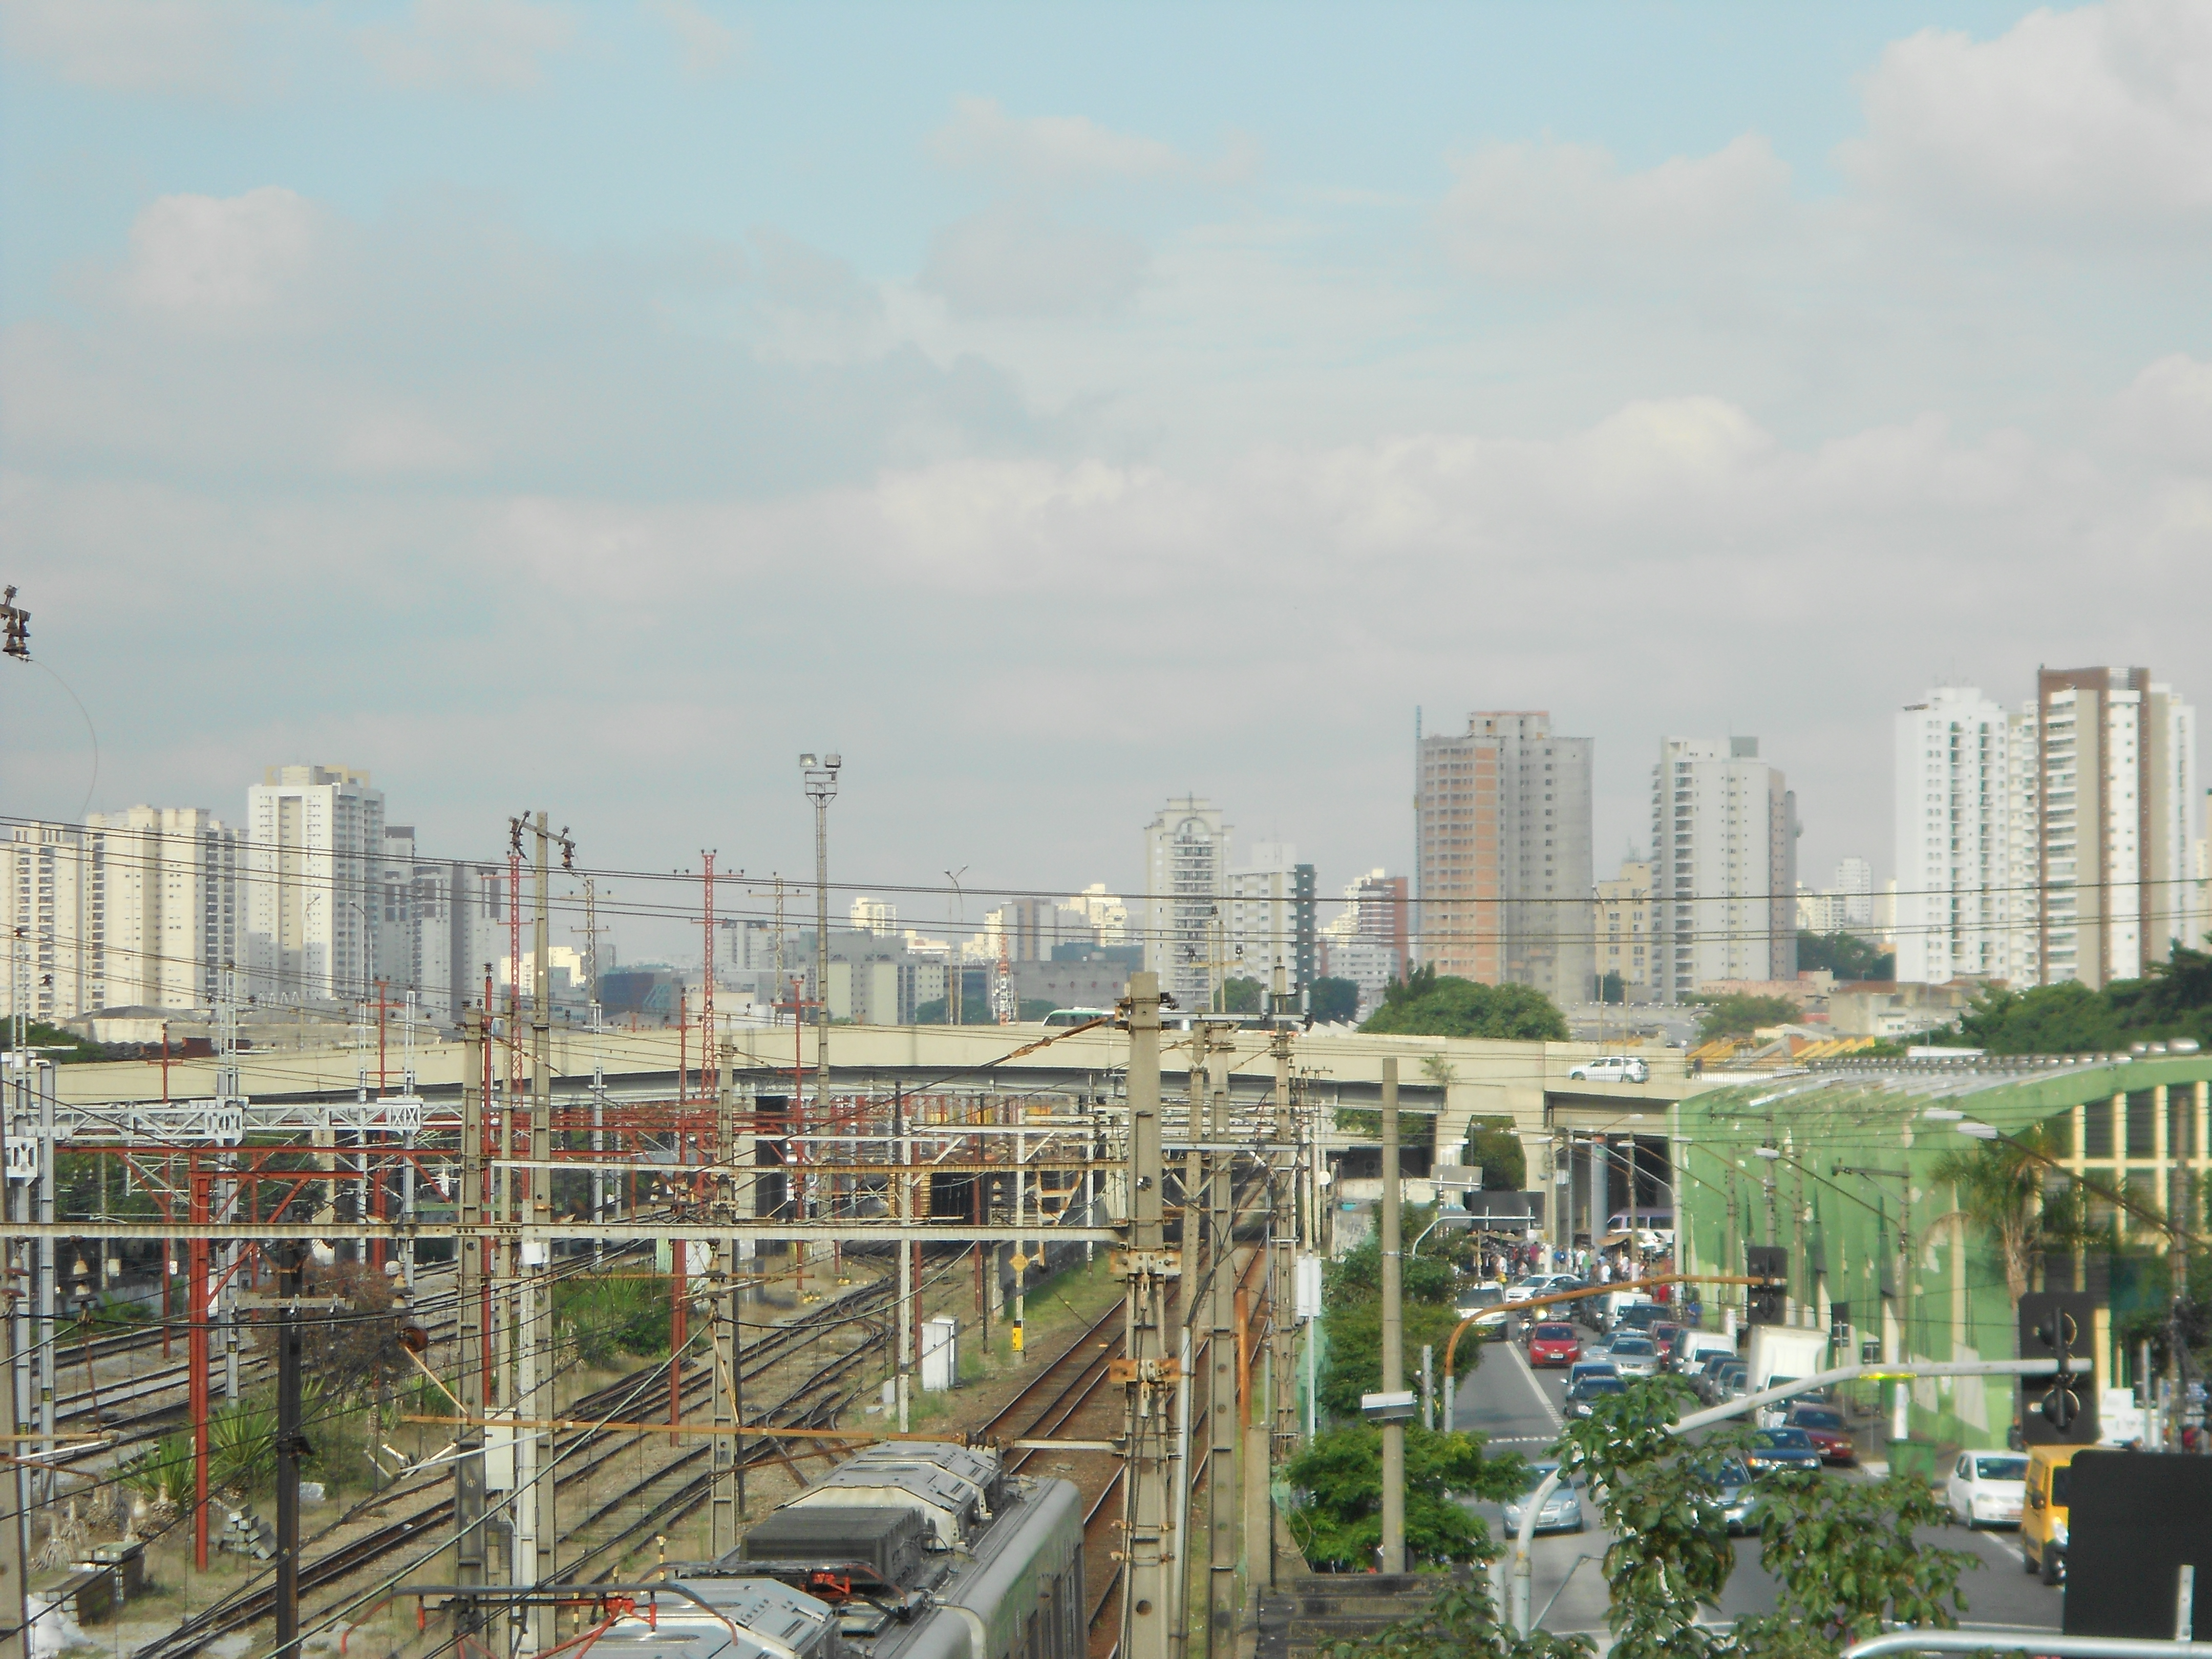
\includegraphics[keepaspectratio,width=\textwidth]{fotos/DSCN7767.JPG}
	\end{figure}	
	
	\subsubsection{Distrito da Barra Funda}
	
	Conforme comenta \citeonline[pág. 19]{Brunelli}, no final do século XIX ``as indústrias instalaram-se ao longo dessas ferrovias e, conseqüentemente, acompanharam-nas os bairros operários, dentre eles o da Barra Funda'', destaca ainda que devido às políticas higienistas e segregacionistas da elite econômica e política de outrora, ``no bairro da Barra Funda localizava-se um dos principais	territórios negros da cidade'' \cite[pág. 19]{Brunelli}. Além de destacar o surgimento da Estrada de Ferro Sorocabana, que deu origem à atual Linha 8, \citeonline[pág. 24]{Brunelli} explica que ``a Barra Funda teve toda sua história ligada ao aparecimento dos diversos meios de transporte na cidade, sendo um retrato da completa falta de planejamento do setor e do absurdo de suas diretrizes''.
	
	\noindent
	\begin{minipage}[b]{.4\textwidth}
		\captionof{figure}{Terminal Intermodal Barra Funda, observado a partir do viaduto Antártica, 2013}
		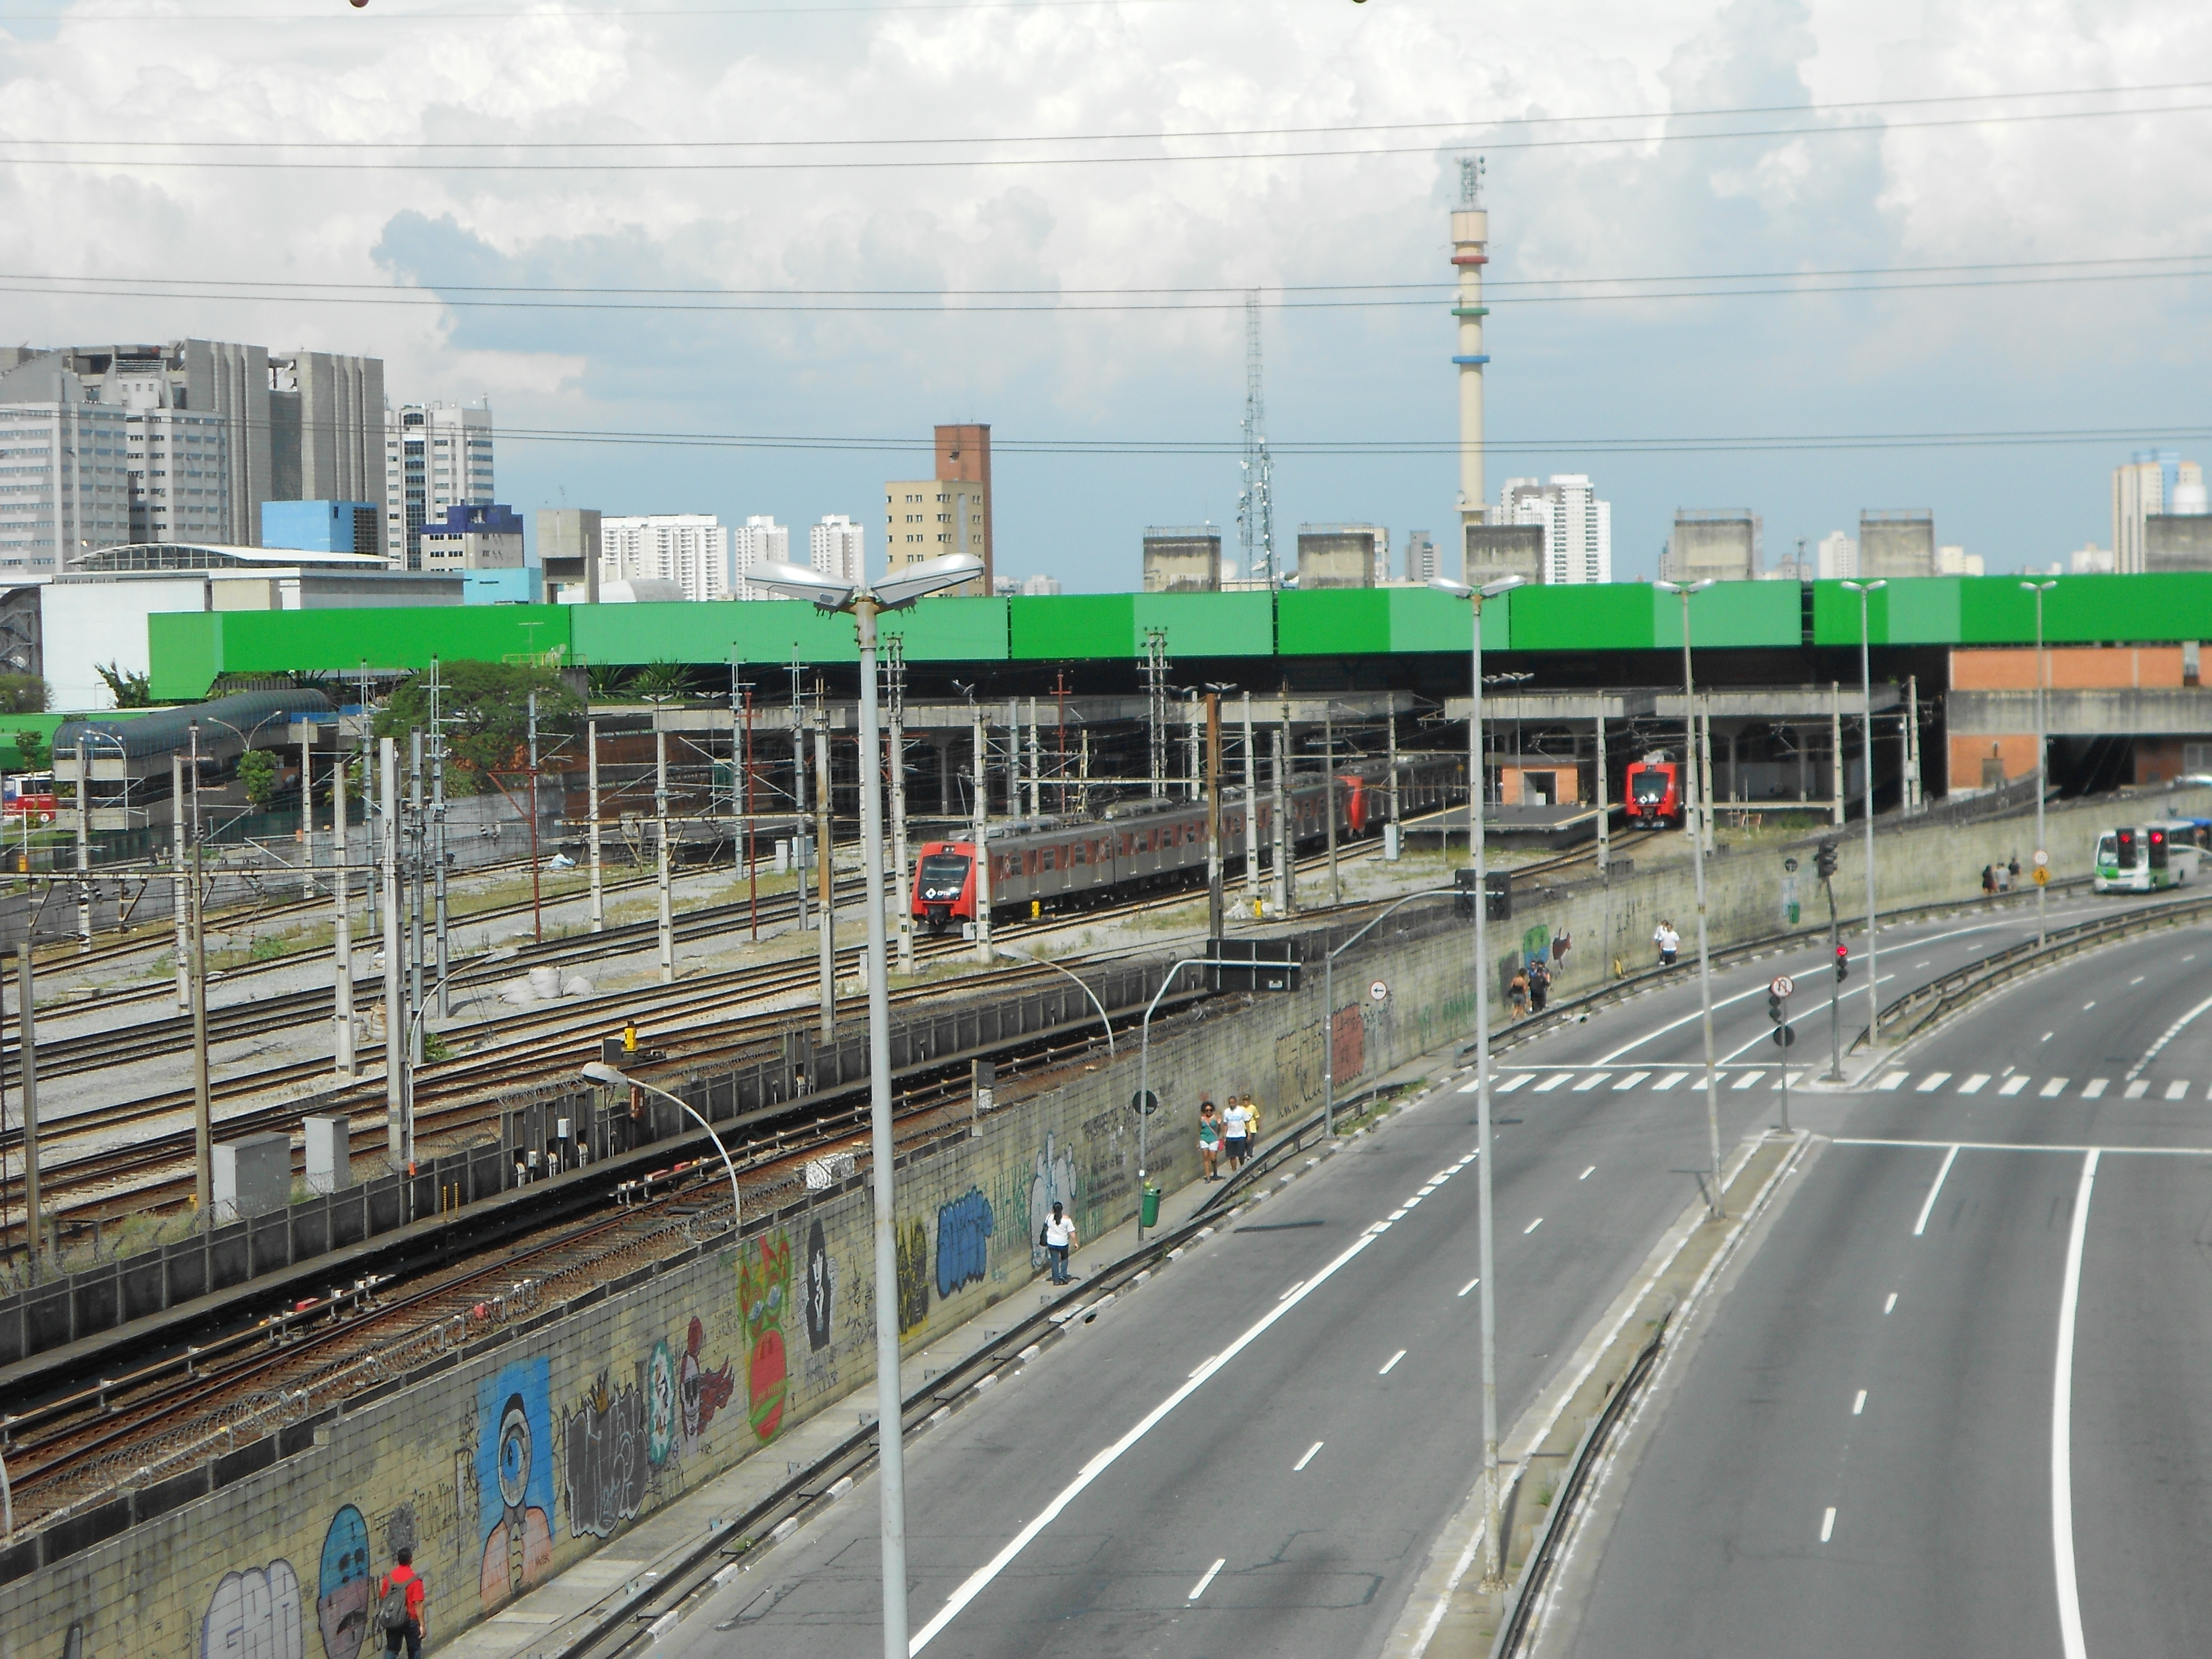
\includegraphics[width=\linewidth]{fotos/DSCN1921.jpg}
	\end{minipage}%
	\hfill
	\begin{minipage}[b]{.4\linewidth}
		\captionof{figure}{Nova edificação sendo erguida junto à Av. Francisco Matarazzo, observada a partir do viaduto Antártica, 2013}
		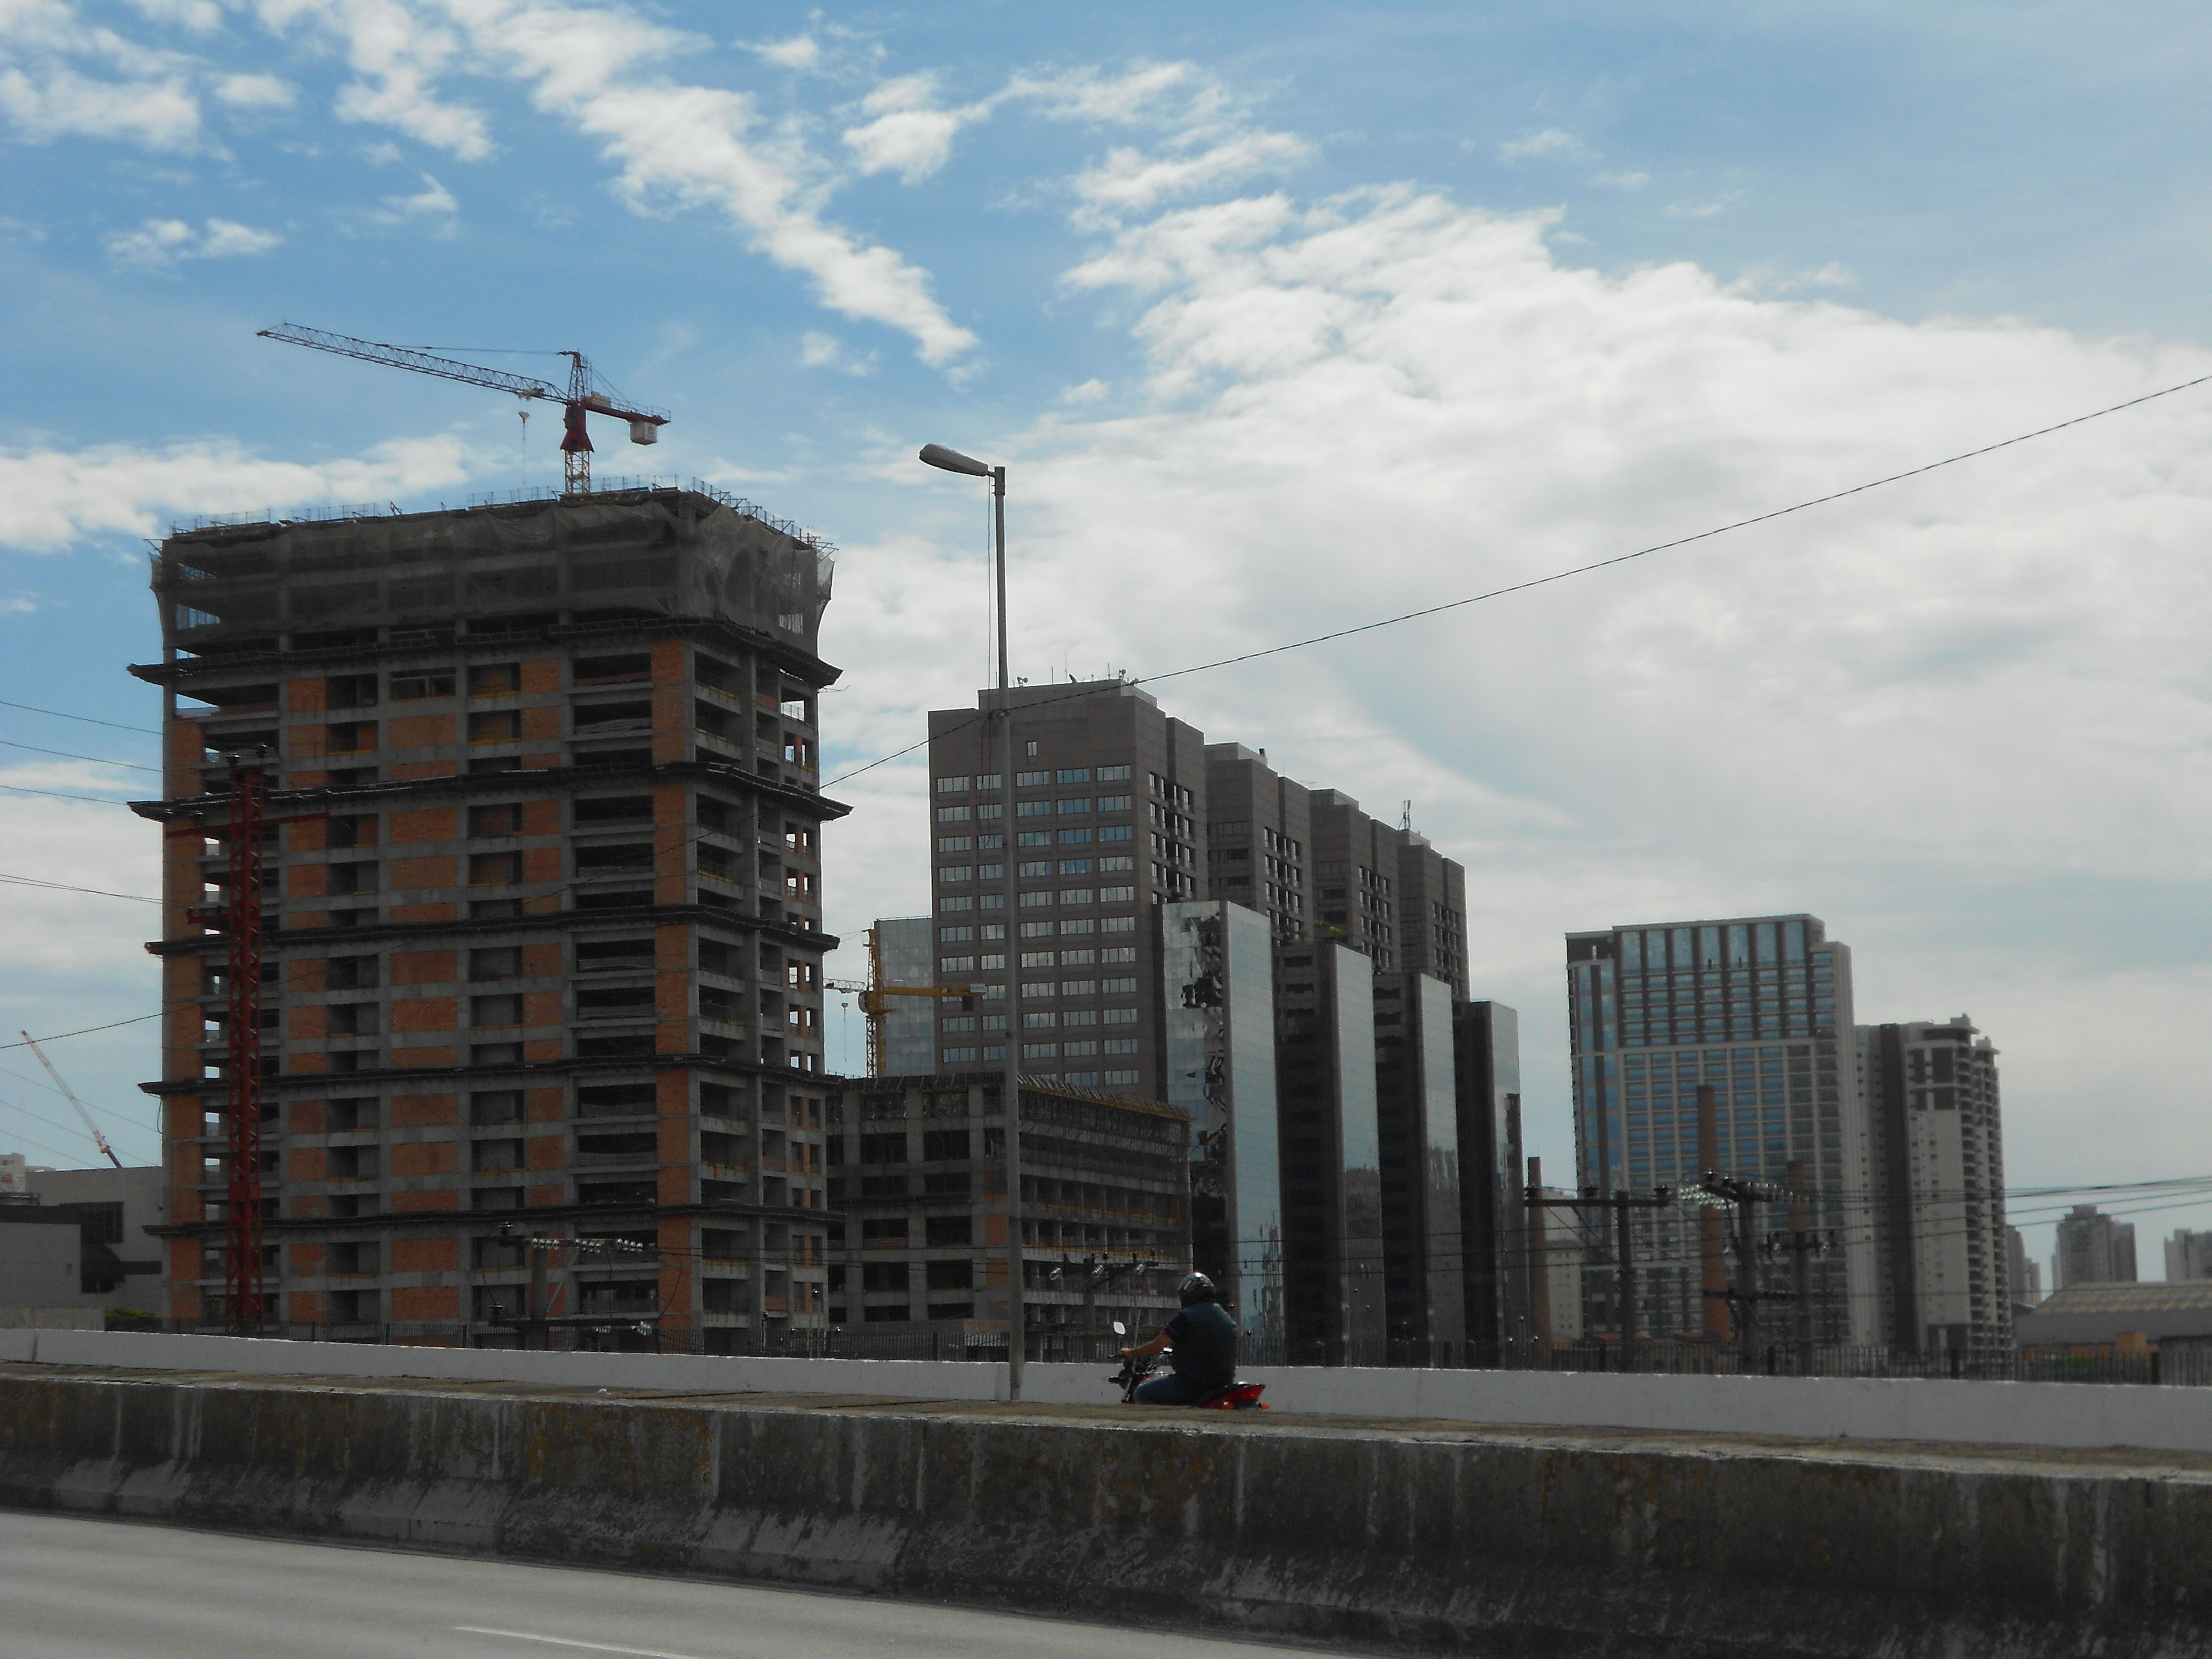
\includegraphics[width=\textwidth]{fotos/DSCN1929.jpg}
	\end{minipage}
	
	Quando da inauguração do prédio da estação atual da Linha 8, que também significou o início do atendimento da \gls{cmsp}, ``Luiz Antônio Pompéia (\gls{embraesp}) afirmou: “A Barra Funda está destinada a um boom imobiliário fantástico nos próximos anos (\dots) poderia ser tão atraente
	quanto Perdizes (...) É um bairro bem servido por avenidas, pelo transporte urbano, próximo ao centro. O que mais alguém pode querer?” 16 Na mesma reportagem, o presidente do Metrô à época afirmava: ``O certo é que, em cinco anos, a Barra Funda será outro bairro''' \cite[pág. 26, com menção a Veja São Paulo, 25/11/87, pág. 24]{Brunelli}, entretanto, ``apesar do início do funcionamento da linha Leste-Oeste do Metrô, em 1988, da construção do Terminal Intermodal da Barra Funda \textemdash o maior da cidade \textemdash da Rodoviária Oeste, e da inauguração do Memorial da América Latina (projeto de Oscar Niemeyer), os resultados dessas melhorias ainda não são evidentes, inobstante de já se terem passado mais de dez anos, alterando muito pouco o perfil do bairro, aparentemente parado no tempo'' \cite[pág. 30]{Brunelli}.
	
	Finalmente, \citeonline[pág. 93]{Brunelli} comenta que ``há um visível desenvolvimento comercial e institucional, notadamente na avenida Marquês de São Vicente e proximidades, e na avenida Dr. Abrahão Ribeiro. Sua importância vai além dos limites distritais, uma vez que favorecem o acesso às Rodovias Presidente Dutra, Ayrton Senna, Castelo Branco, Anhangüera e Bandeirantes'', o que se deve, segundo \citeonline[pág. 93]{Canutti} às obras viárias concluídas na década de 1970, que melhoraram sua conectividade com as zonas central e norte. bem como facilitaram o acesso à orla ferroviária e a própria transposição desta, exemplos de obras segundo \citeonline[pág. 93]{Canutti} são a construção do Viaduto Antártica, a abertura da Rua Quirino dos Santos e melhoramentos na própria Marquês de São Vicente. \citeonline[pág. 93]{Canutti} também aponta que as obras viárias tiveram caráter metropolitano.

	\noindent
	\begin{minipage}[b]{.4\textwidth}
		\captionof{figure}{Av. Marqu\^{e}s de S\~{a}o Vicente X Viad. Ant\'{a}rtica, 2016}
		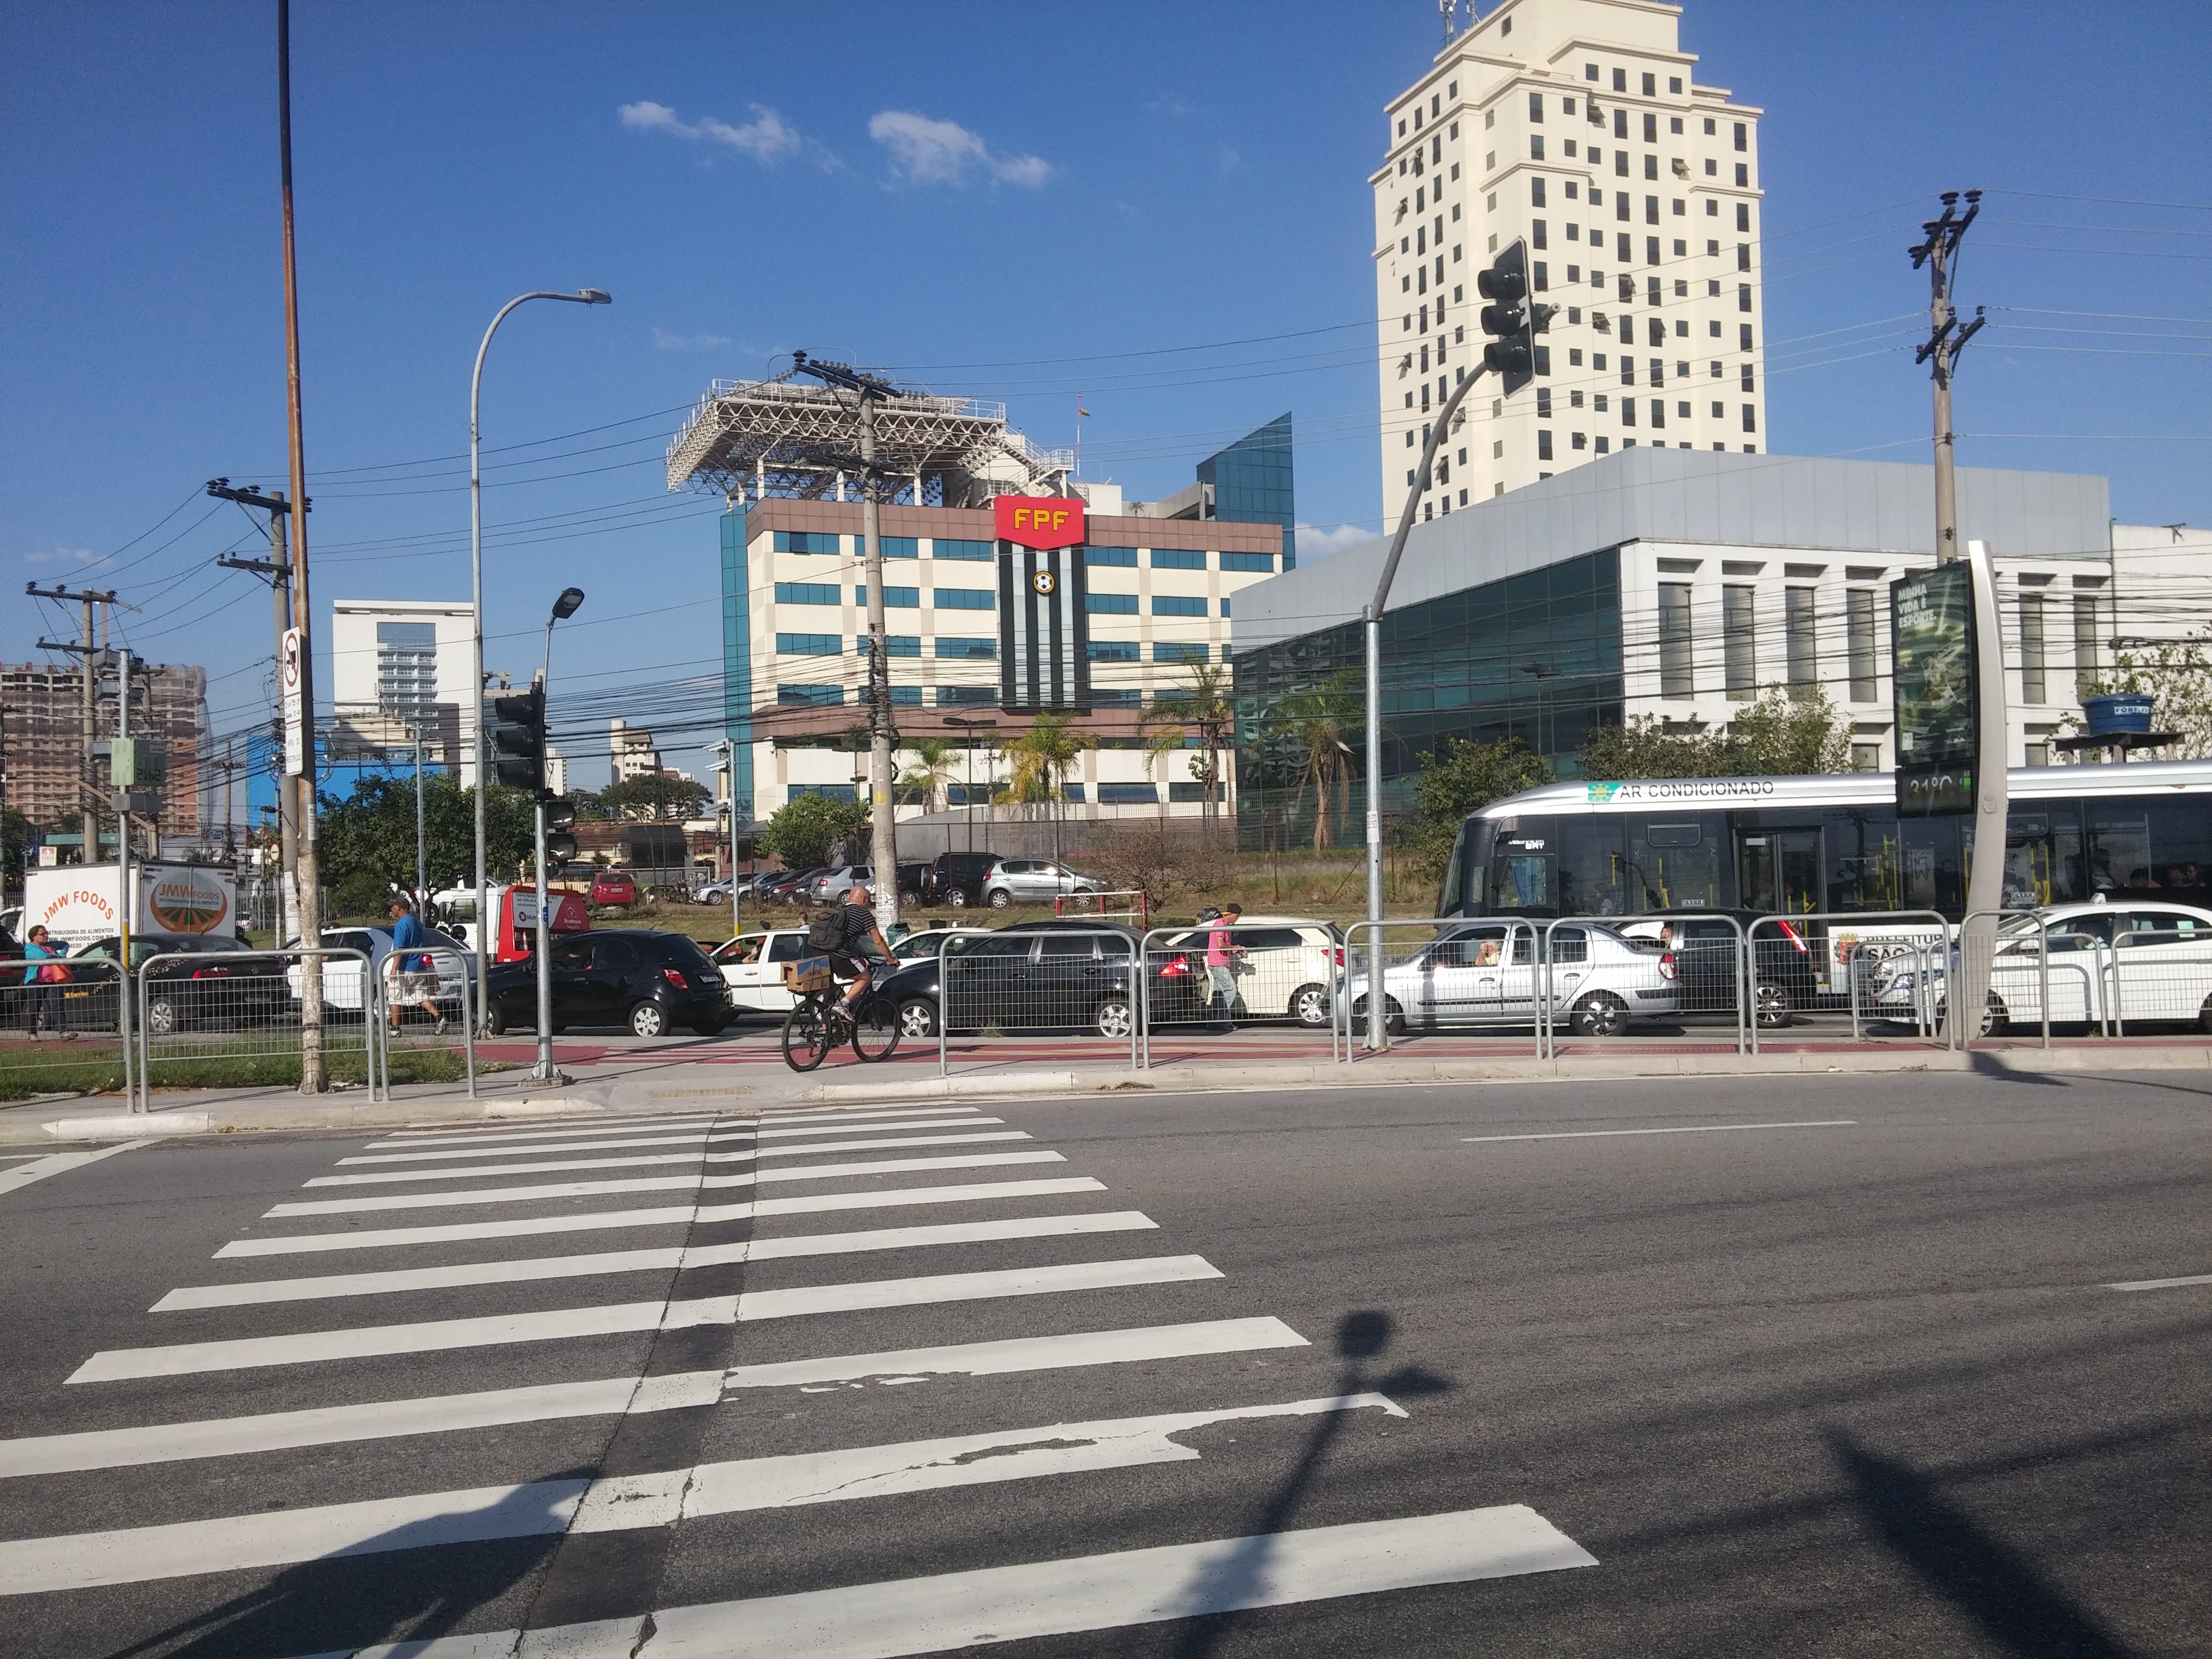
\includegraphics[width=\linewidth]{fotos/20160712_150346.jpg}
	\end{minipage}%
	\hfill
	\begin{minipage}[b]{.4\linewidth}
		\captionof{figure}{Avenida Marqu\^{e}s de S\~{a}o Vicente, 2017}
		\includegraphics[width=\textwidth]{fotos/2017_04_23_001.jpg}
	\end{minipage}
	
	Contemporizando, segundo \citeonline[149]{Ottoni}, ``aproveitando-se de um novo posicionamento do mercado imobiliário em relação à região, que passou a ser vista como possível novo polo residencial, foi lançado, em março de 2008, um shopping center pelo grupo gaúcho Zaffari, o Shopping Bourbon, com 10 salas de cinema e teatro; o shopping center, com cerca de 33.000 m2, construído no terreno onde se localizava o antigo Shopping Center
	Matarazzo''. Vale aqui dizer que, antes dessas transformações ocorridas na primeira década do novo milênio, a quadra mais adensada não ia além de uma configuração urbana contínua a Perdizes, na outra face da orla ferroviária, junto à Avenida Francisco Matarazzo, sendo o Shopping Center West Plaza inaugurado em 1991 \cite[77]{Ottoni}.
	
	\subsubsection{Distrito da Lapa}
	
	\citeonline[pág. 102]{planocentro} traça um panorama geral sobre a Lapa, reiterando a importância do transporte sobre trilhos:
	
	\begin{citacao}
		O Bairro da Lapa tem seu desenvolvimento intimamente ligado à implantação da ferrovia e posteriormente ao acesso a várias rodovias que interligam a cidade ao interior do Estado e a outros Estados do país. As primeiras indústrias surgiram ao longo da linha do trem que corta longitudinalmente o seu território. Ao redor das indústrias surgiram vilas operárias que abrigavam os seus trabalhadores.
		
		Esta ocupação desenhou o território marcado por grandes lotes e quadras com características de ocupação industrial, com sistema viário generoso nas suas dimensões, porém com poucas vias. A disponibilidade de equipamentos público urbanos básicos era escassa em função da reduzida população residente.
	\end{citacao}
	
	\noindent
	\begin{minipage}[b]{.4\textwidth}
		\captionof{figure}{Centro Comercial da Lapa, 2015}
		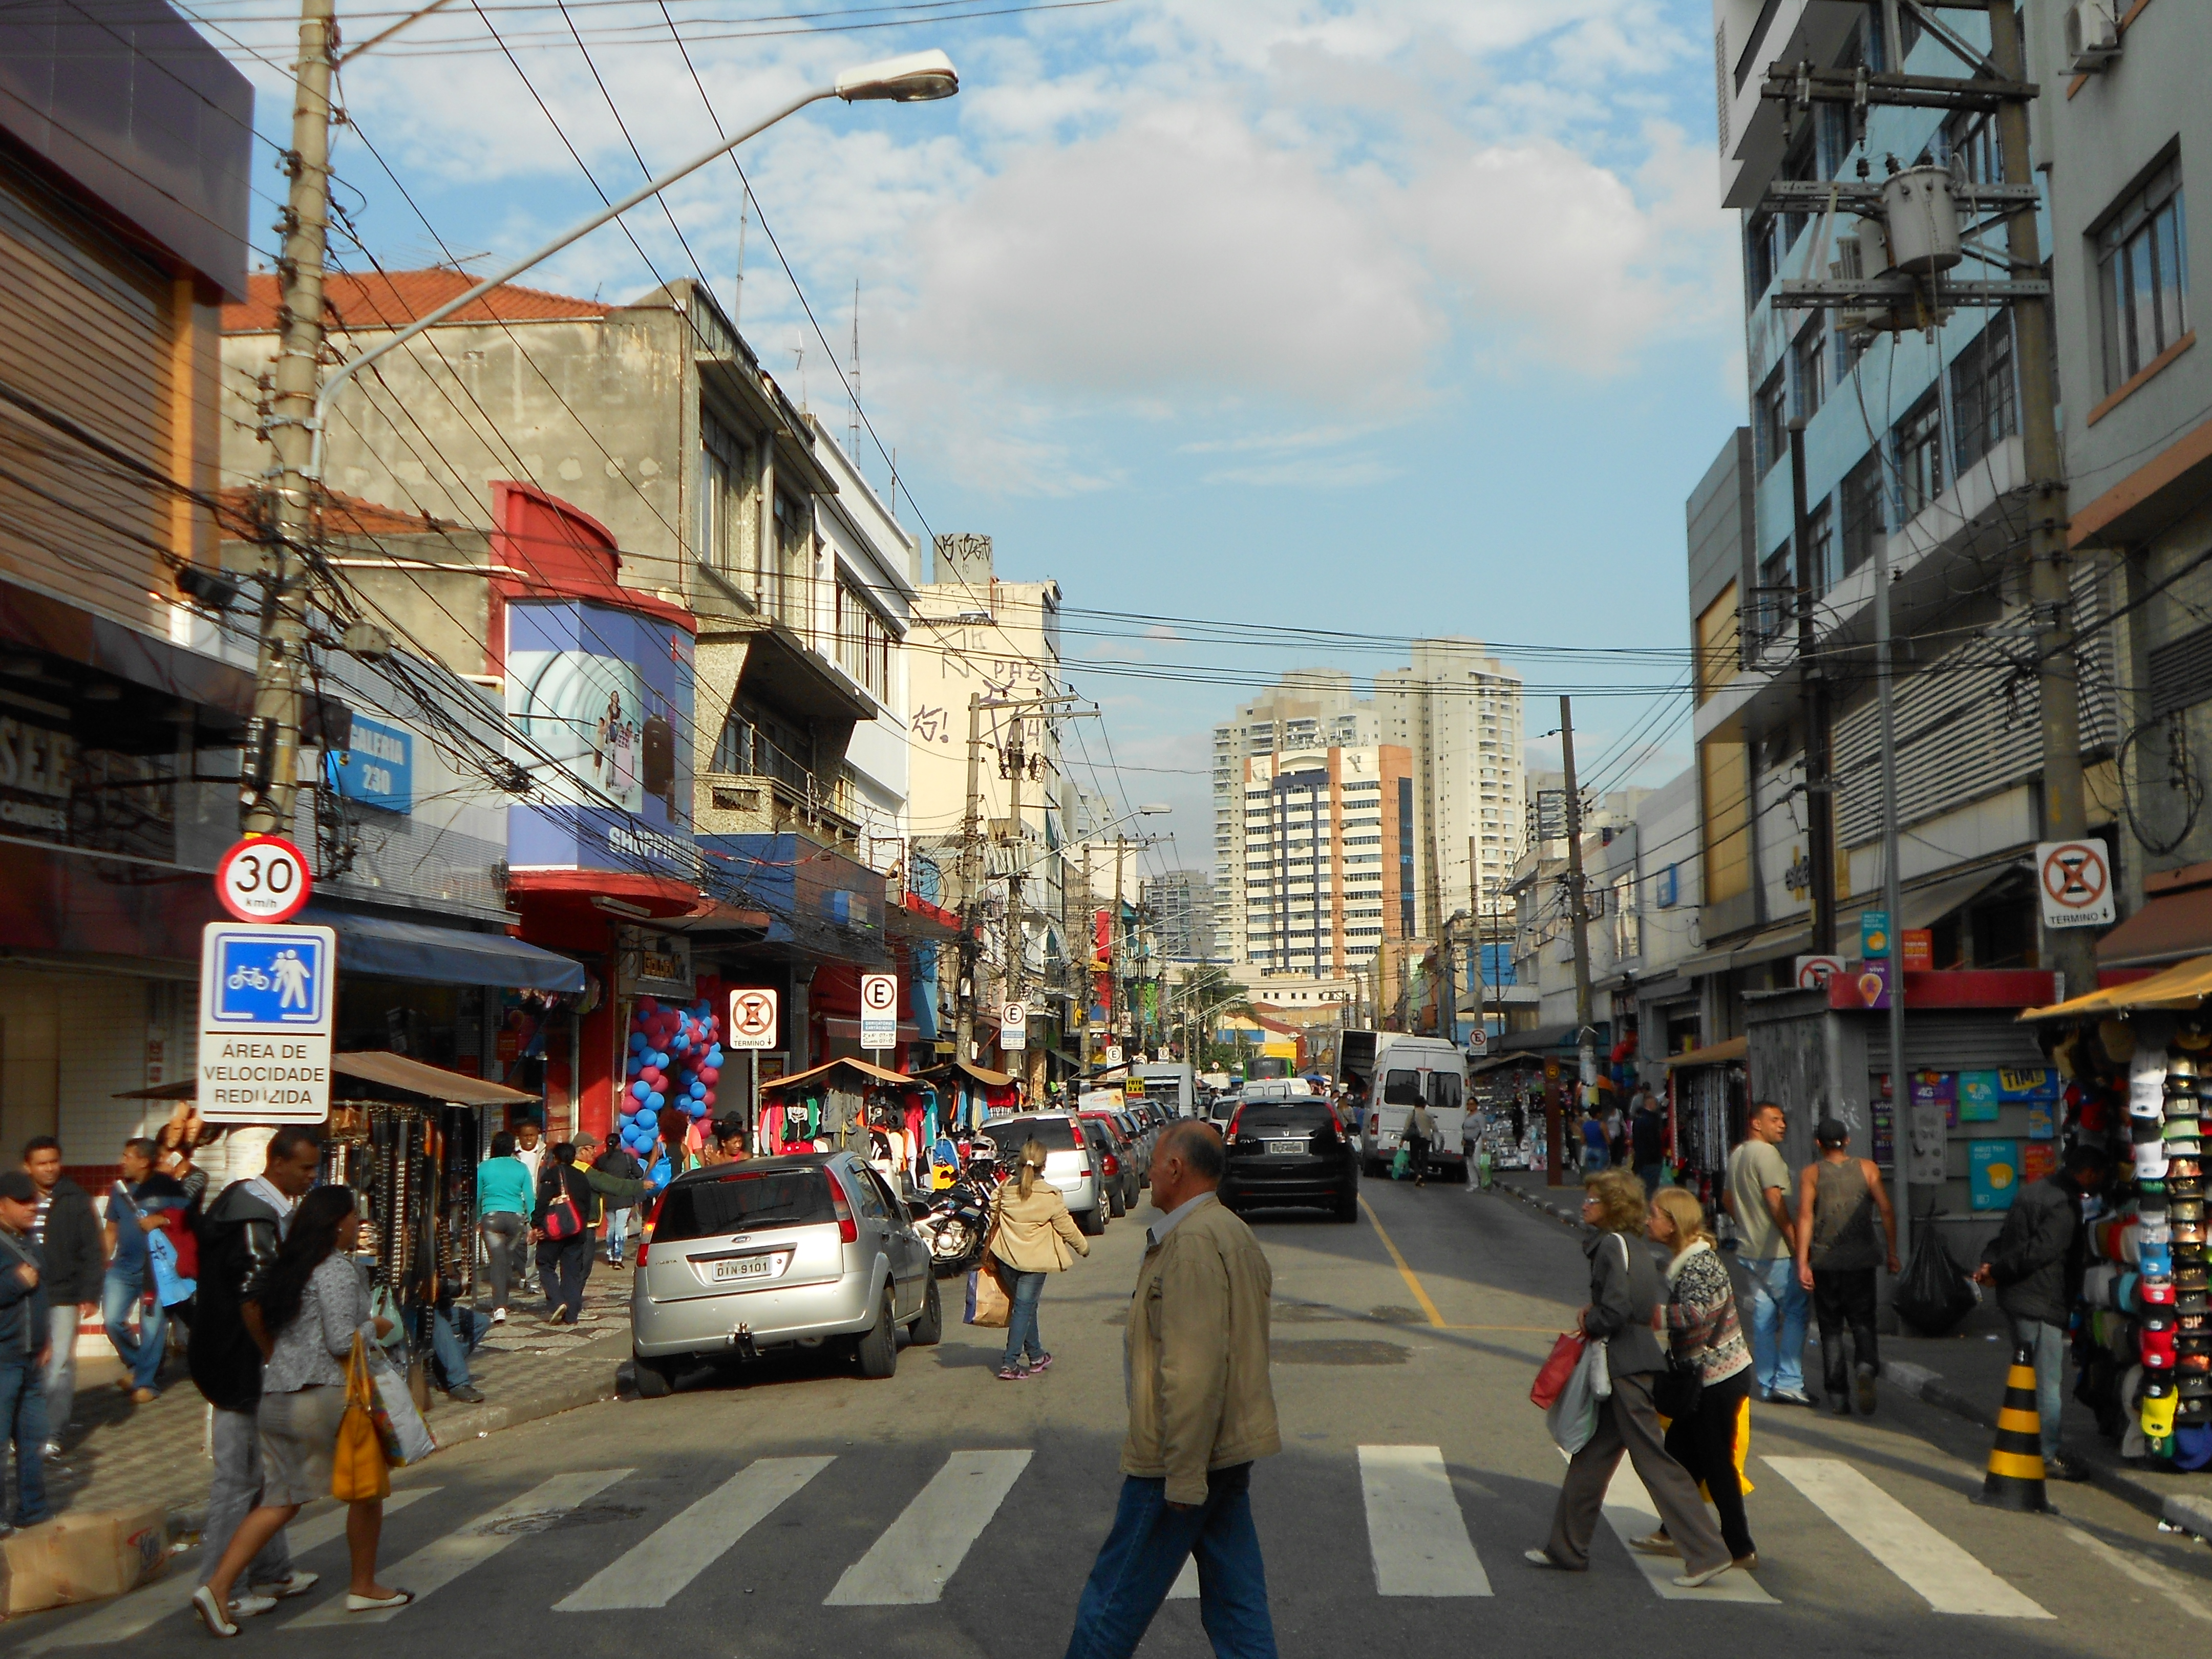
\includegraphics[width=\linewidth]{fotos/DSCN7783.jpg}
	\end{minipage}%
	\hfill
	\begin{minipage}[b]{.4\linewidth}
		\captionof{figure}{Centro Comercial da Lapa, 2015}
		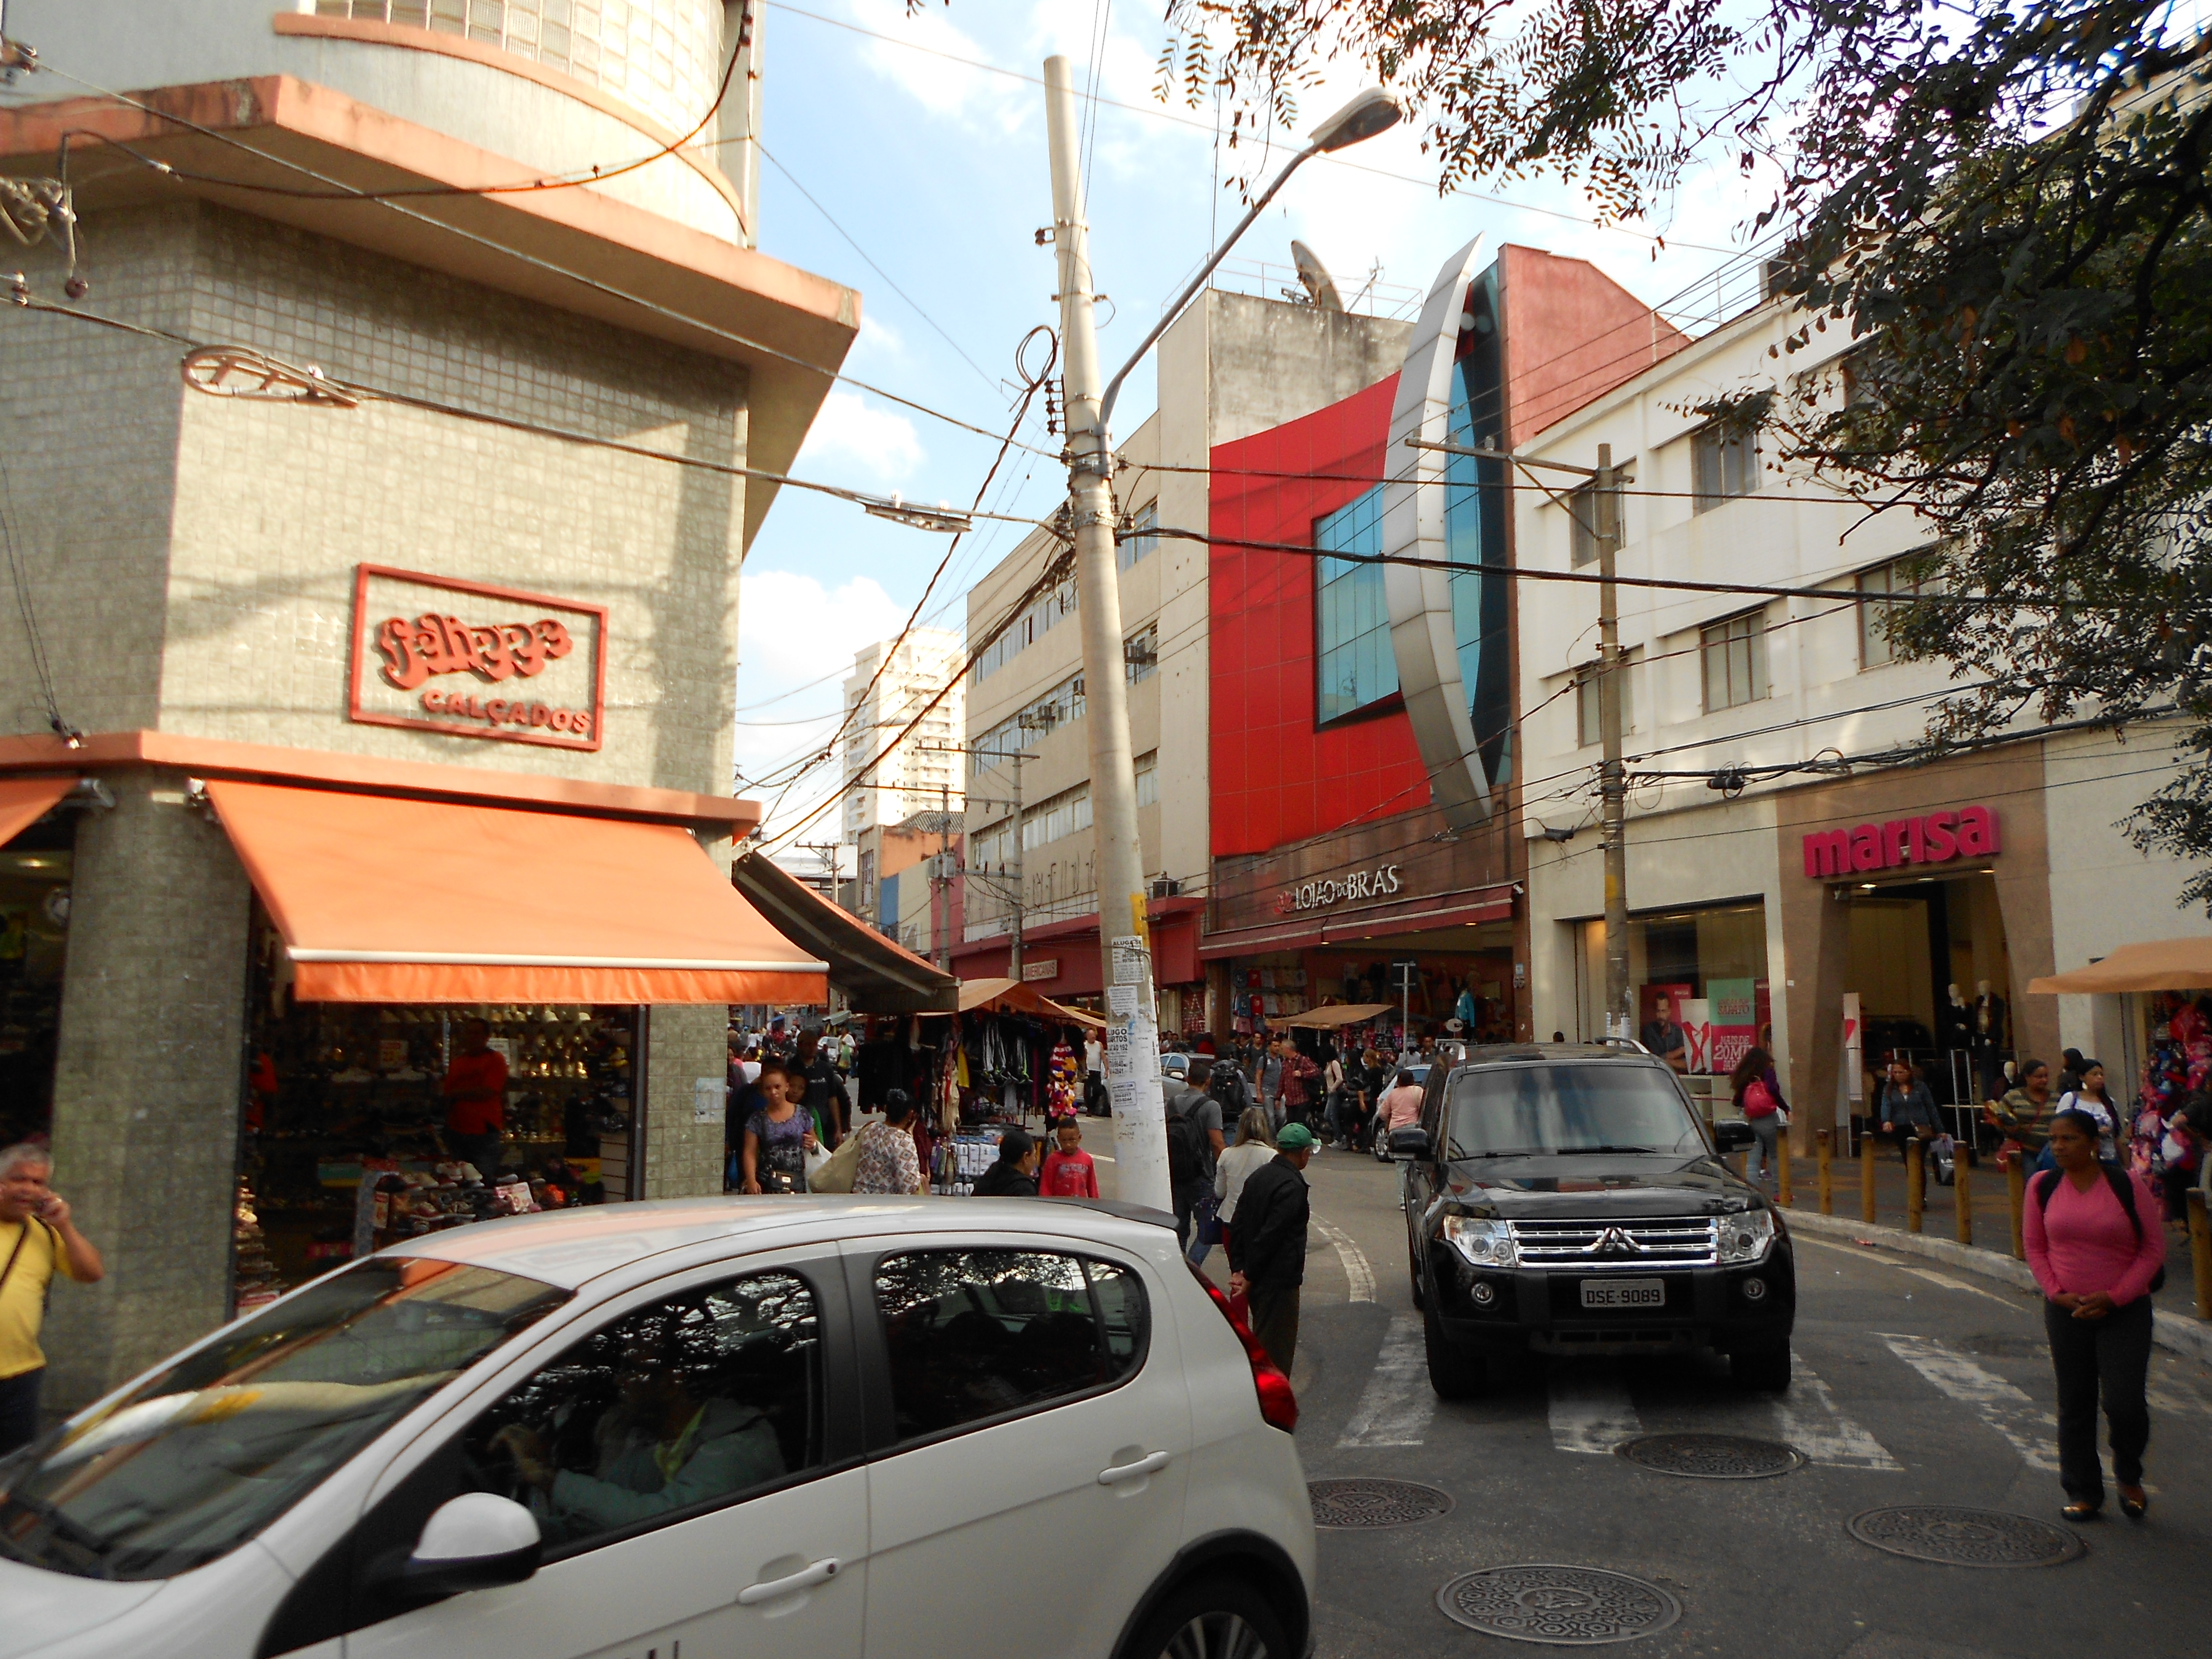
\includegraphics[width=\textwidth]{fotos/DSCN7784.jpg}
	\end{minipage}
	
	A respeito do comércio, ``o centro comercial da Lapa continua como forte concentração de atividades ligadas ao comércio de bens e serviços de atendimento local e diversificado, com a grande presença de lojas de bens duráveis e oficinas prestadoras de serviços, principalmente motivados pela grande acessibilidade promovida pelo cruzamento de inúmeras linhas de ônibus e a estação ferroviária da \gls{cptm}'' \cite[pág. 103]{planocentro}.


	\section{Linha 9-Esmeralda} \label{L9}
	
	\subsection{Lapa}
	
	No que diz respeito ao atendimento da Prefeitura Regional da Lapa, a Linha 9 se limita à Estação CEASA, de forma que maiores detalhes podem ser conferidos na seção \ref{Lapa} do capítulo \ref{L8}.
	
	Dado o limitado atendimento prestado pela Linha 9, vale apontar que ``a atividade comercial, porém se espalhou por todo o bairro principalmente através de pequenos estabelecimentos de atendimento de necessidades cotidianas ao longo principalmente da Vila Romana e Vila Leopoldina, ligadas ao surgimento dos edifícios residenciais'' \cite[pág. 103]{planocentro}.
	
	\subsection{Pinheiros} \label{Pinheiros}
	
	Segundo \citeonline[pág. 147]{planocentro}, ``localizada no vetor oeste da cidade, a Subprefeitura Pinheiros tem área de cerca de 3.170 ha distribuídos por quatro distritos: Alto de Pinheiros, Jardim Paulista, Itaim Bibi e Pinheiros''.
	
	No que diz respeito à infraestrutura de circulação, a região é ``atendida por duas linhas de metrô, uma de trem e por dois corredores de ônibus. Apesar disso, 60\% das viagens diárias de seus habitantes são feitas pelo modo individual. É cortada pelo trânsito de passagem do sistema radiocêntrico da cidade, provocando conflitos de uso e com o transporte coletivo. Possui diversas vias estruturais - que conectam rodovias e outros bairros da cidade, muitas vias coletoras e poucas vias locais'' \cite[pág. 147]{planocentro}.

	\citeonline[pág. 13]{Ferreira} explica que a partir dos anos 1970 o setor industrial localizado no centro metropolitano perdeu importância, de forma que o setor terciário, muito menos concentrado e homogêneo no território, absorveu sua mão de obra, o que se traduz em menor polarização, novas localizações (o autor cita shoppings centers e centros empresariais, por exemplo) e alterações significativas no uso do solo \apud[pág. 25]{Ferreira}{Mello}, o que pode ser relacionado com o processo de rentismo urbano sublinhado por \citeonline[pág 30, nota de rodapé 2]{Acselrad}, no qual ocorre gentrificação estratégica de áreas urbanas outrora industrializadas e marcadas pelo desinvestimento. A gentrificação se dá a partir das possibilidades econômicas, tanto para valorização, como para aquisição de propriedades imobiliária, num processo que exclui moradores de menor renda \apud[pág. 28-29]{Acselrad}{Arantes}. O trecho central da Linha 9-Esmeralda, que avança ao longo da Avenida das Nações Unidas por regiões enobrecidas e substancialmente modificadas pelo processo, é emblemático, não por se encaixar no fenômeno que acaba de ser descrito, como também pela extensão do território afetado, que pode ser observado utilizando as estações da CPTM como referência, visto que não há, exceto pela Linha 4-Amarela da \gls{cmsp} em regime de concessão patrocinada, outra infraestrutura de transporte de alta capacidade.
	
	\begin{figure}[h]
		\caption{Visão dos empreendimentos imobiliários a partir da plataforma da Estação Cidade Jardim (2013}
		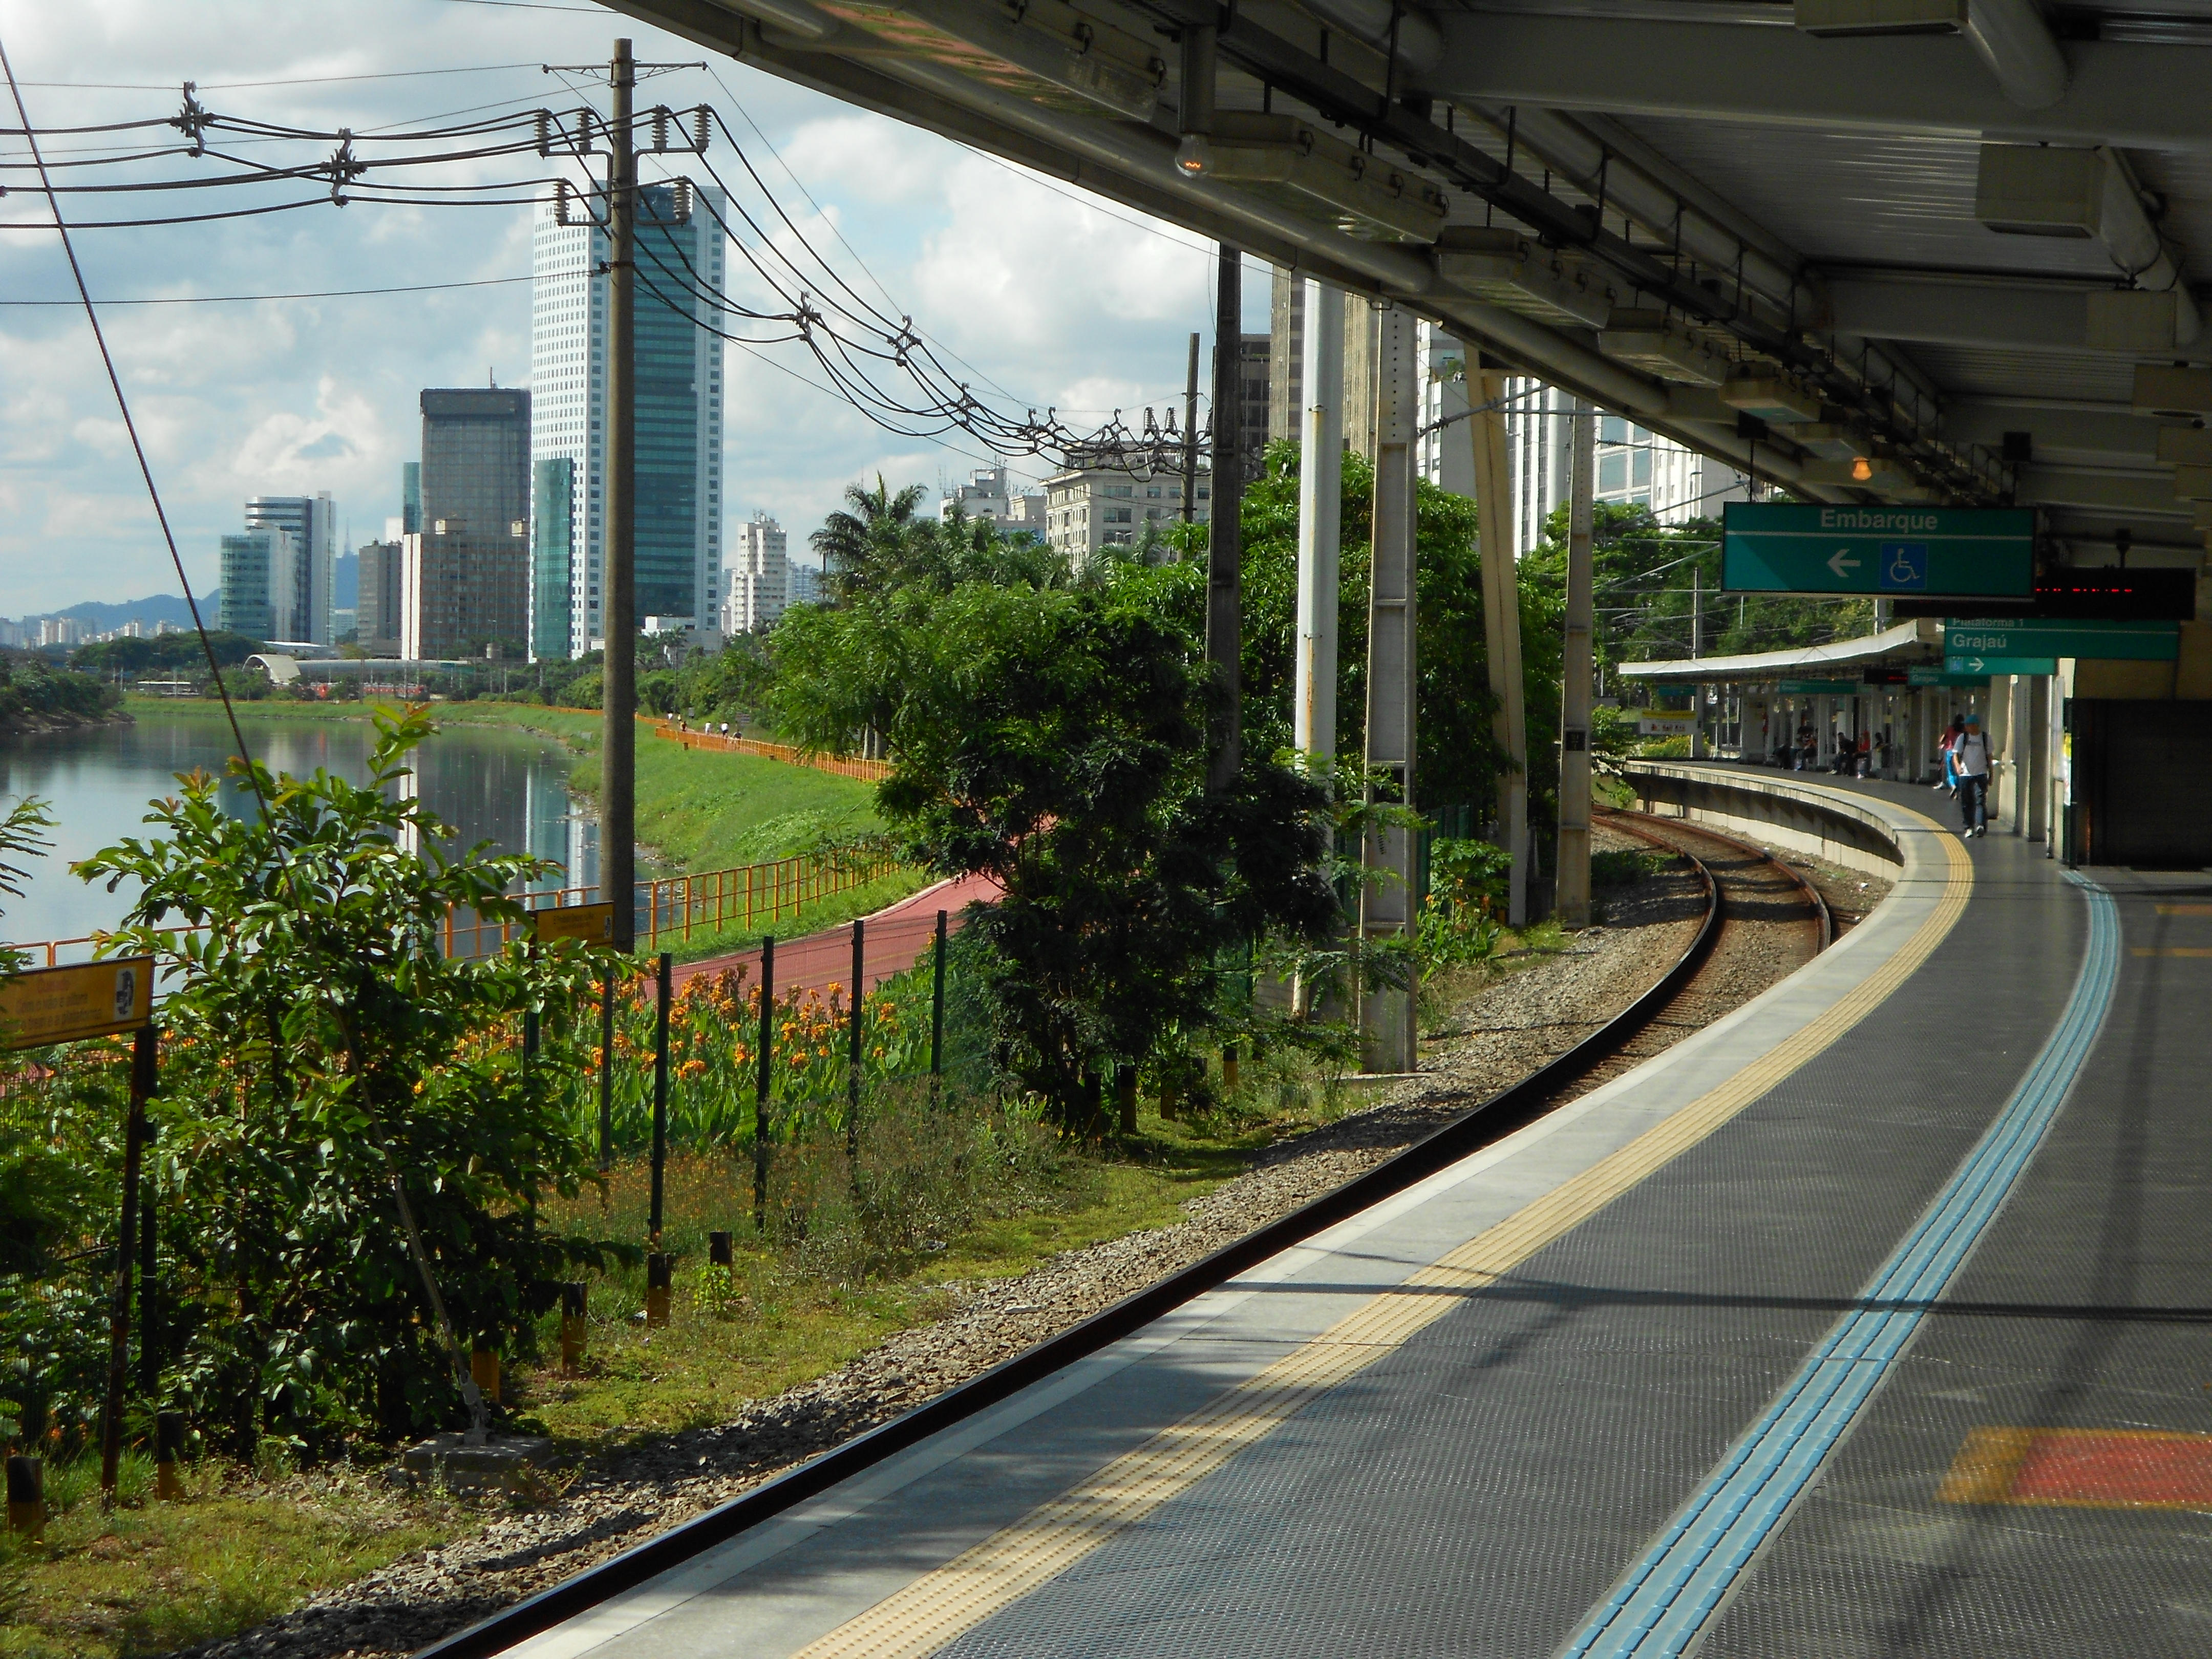
\includegraphics[keepaspectratio,width=\textwidth]{fotos/DSCN2007.JPG}
	\end{figure}
	
	\begin{figure}[h]
		\caption{A Estação Cidade Jardim é vizinha de um dos edifícios residenciais mais caros da capital paulista (2013)\cite{apecaro}}
		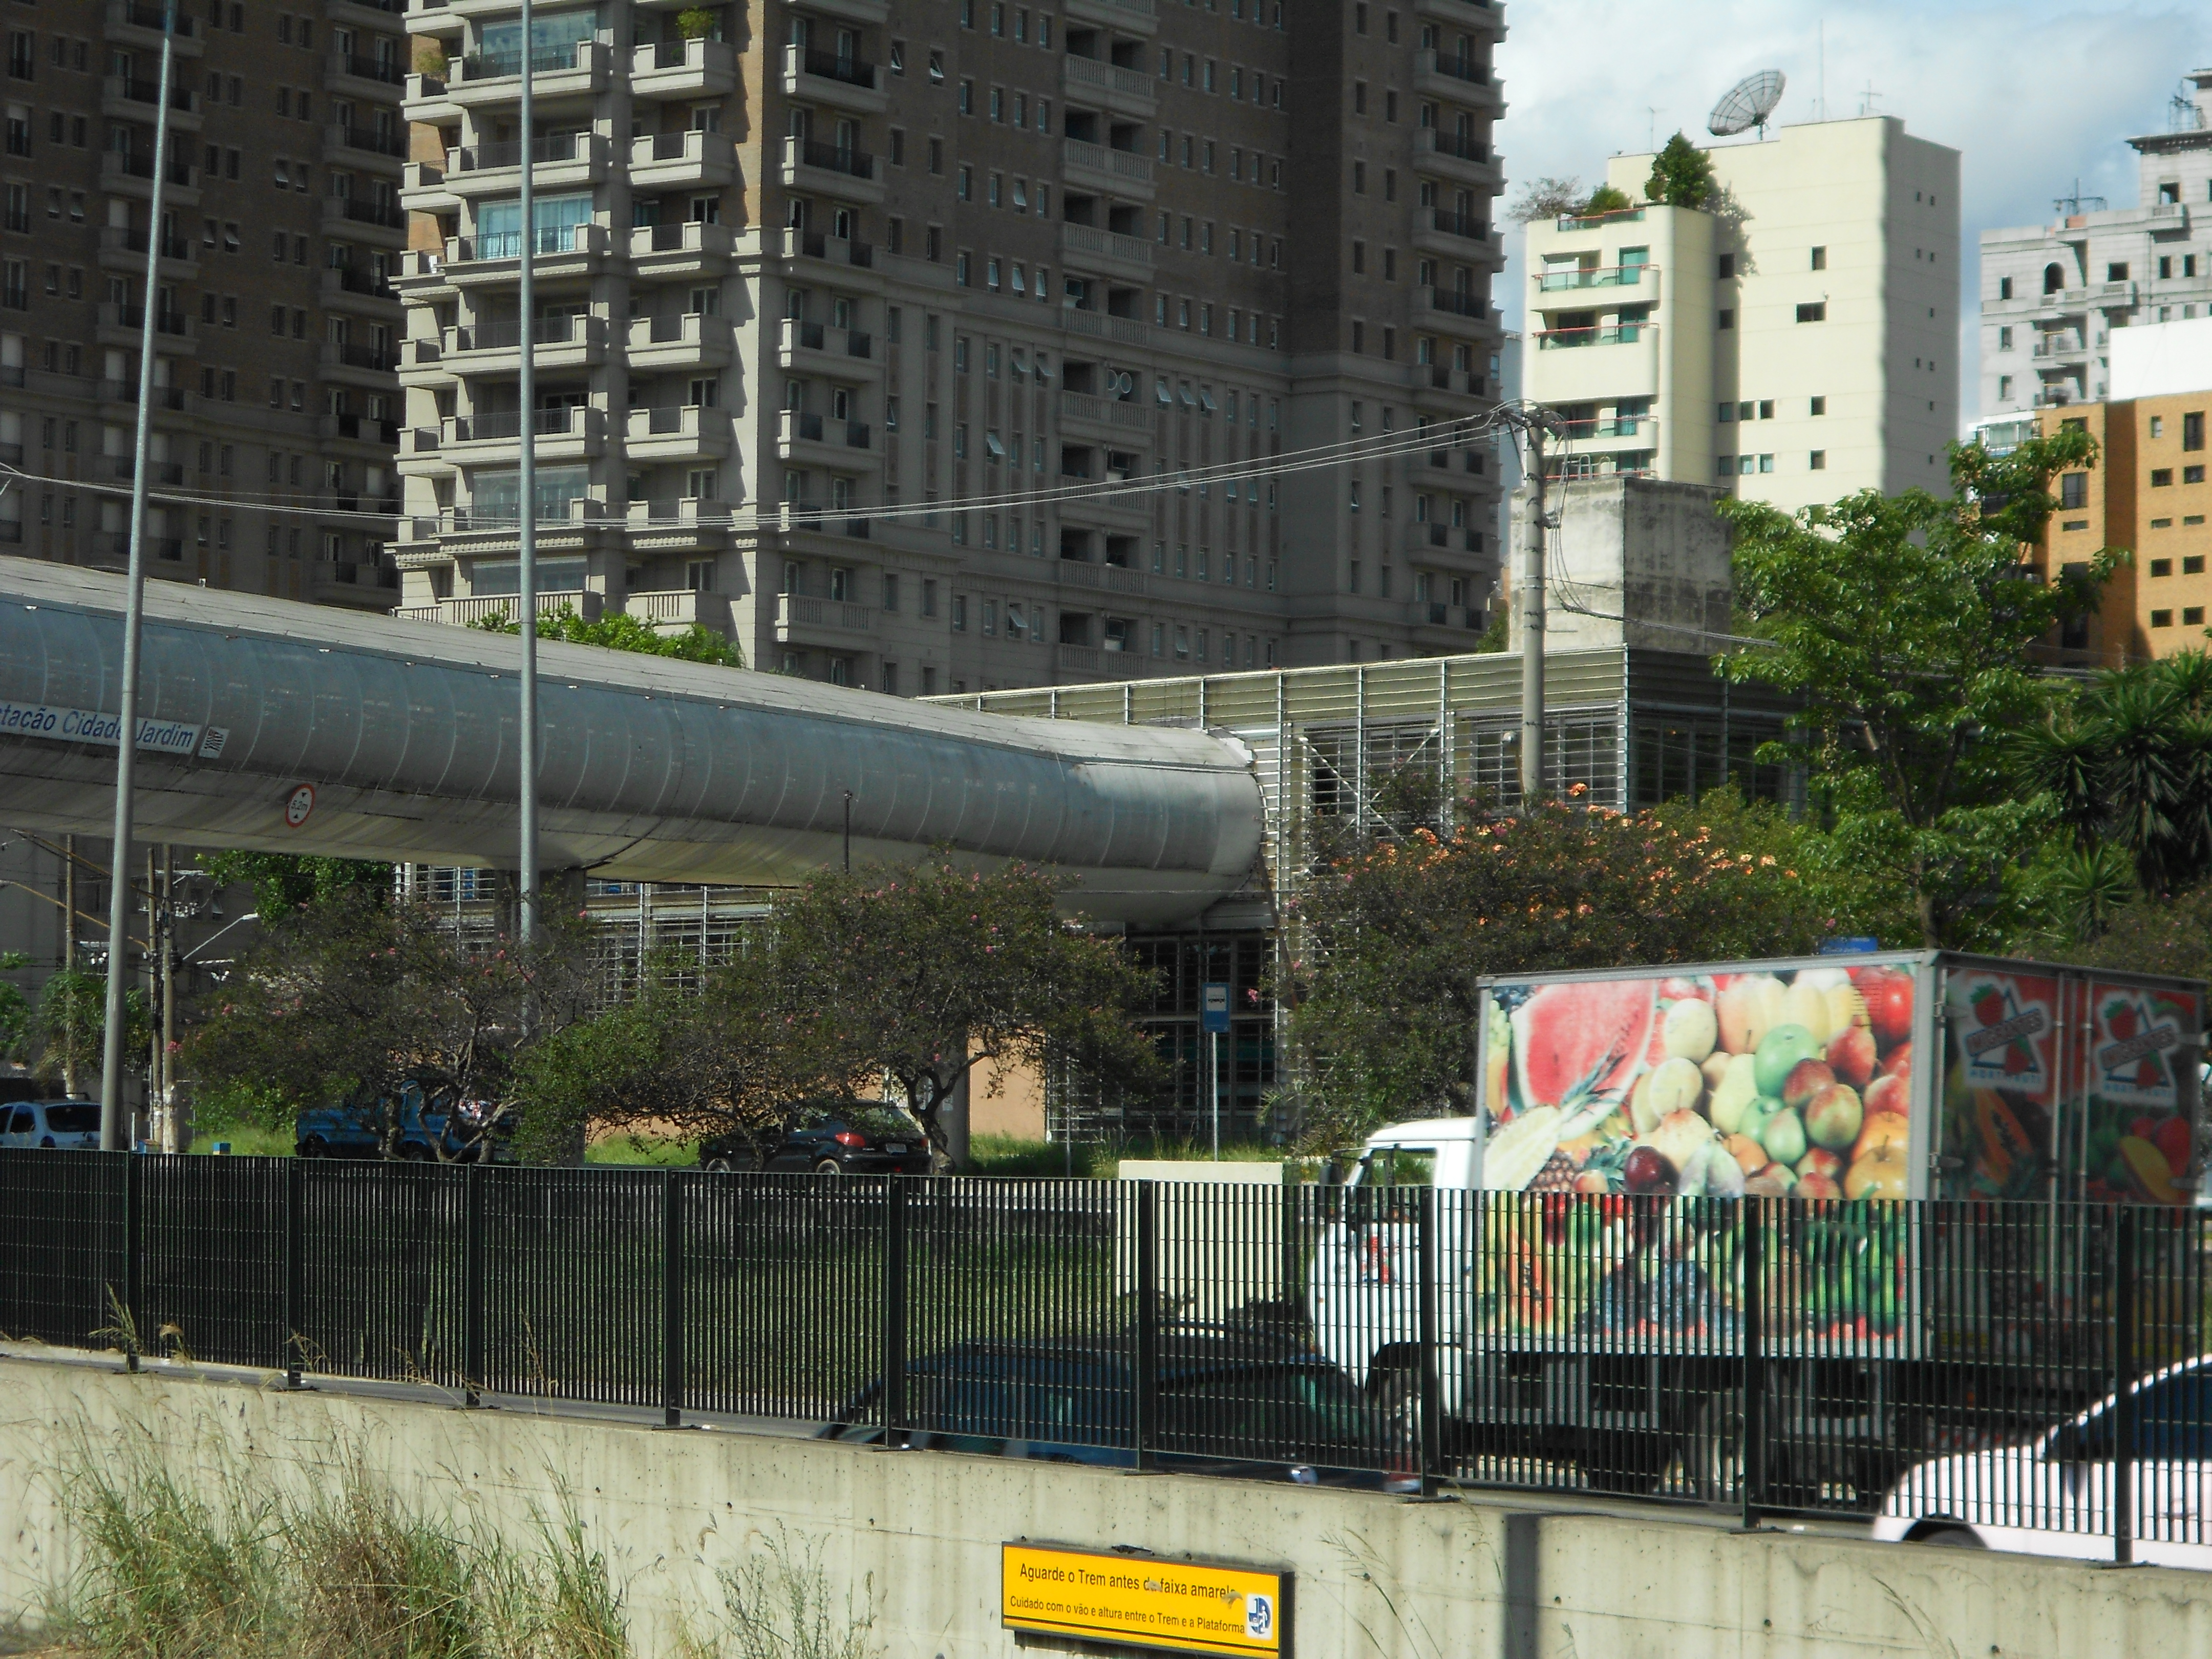
\includegraphics[keepaspectratio,width=\textwidth]{fotos/DSCN2000.JPG}
	\end{figure}	
	
	\citeonline[pág. 201]{Frugoli} destaca a pressão e o desejo de um ator ligado à iniciativa privada com relação à Linha 9, ainda antes do término de sua dinamização, que resultou, sobretudo, na construção e inauguração das estações Hebraica-Rebouças, Cidade Jardim, Berrini, Morumbi, Granja Julieta, Socorro e Vila Olímpia\cite[pág. 38]{Ferreira}: ``"-- A linha de metrô está pronta. Está aí no Rio Pinheiros, a linha de trem. Não sei por que, até agora, as nossas "autoridades"\dots Eu acho que os caras não têm visão nenhuma, é uma coisa impressionante. É só fazer algumas estações e está pronta. Não, eles vão fazer, mas só quando fizerem a da Rebouças. Faz já! (Entrevista com Carlos Bratke, cit.)''.
	
	Apesar da posição colocada por Carlos Bratke, recuperada por \citeonline{Frugoli}, a utilização do transporte coletivo não atinge índices elevados, como podemos ver no perfil a seguir, levantado em 2016 por \citeonline[pág. 152]{planocentro}:
	
	\begin{citacao}
		“Com relação a infraestrutura de transporte coletivo de média (corredor de ônibus) e alta capacidade (metrô e trem) a Subprefeitura é atendida por duas linhas de Metrô (2 – Verde e 4 – Amarela), uma linha de trem (9 – esmeralda) e pelos corredores Rebouças e Santo Amaro/9 de julho. Apesar de ser uma das Subprefeituras mais bem servidas de transporte coletivo, 60\% das viagens diárias de seus habitantes é feita pelo modo individual, sendo que o modo coletivo (19\%) perde inclusive para o modo a pé (20,5\%). Em alguns bairros, em função da largura e declividade das ruas, os veículos que operam no subsistema estrutural de transporte coletivo (padron, articulado e biarticulado) possuem dimensões inadequadas às características da via.
	\end{citacao}
	
	Carlos Bratke, como explica \citeonline{Frugoli}. exibe perfeitamente os efeitos descritos por \citeonline{Acselrad}. criticando o poder público, ao mesmo tempo que também demonstra que não era incomodado pela prefeitura ou pelo governo estadual, atuando livremente na Avenida Engenheiro Luís Carlos Berrini:
	
	\begin{citacao}
		As declarações dos irmãos Bratke e matérias da grande imprensa ao longo das últimas décadas ajudam a tecer um quadro que frisa um caráter de "pioneirismo" e "autonomia" quanto ao poder público:
		
		\begin{citacao}
			No espaço de dez anos, [Carlos Bratke, Roberto Bratke e Francisco Collet] operaram em volta da Avenida Luiz Carlos Berrini, sem a mais remota interferência da prefeitura ou de qualquer poder público, uma pequena revolução urbana -- a mais notável já feita num grande espaço da cidade por um único projeto privado de arquitetura. (Veja SP, 1985:16)
		\end{citacao}
		
		Na mesma matéria, Carlos Bratke afirma: "Nunca fui procurado por nenhum órgão público para saber quais são os meus planos" (Veja SP, 1985:21).

		\begin{citacao}		
			"Essa avenida não é um planejamento urbano. Precisavam fazer um canal, então fizeram essa avenida que ligava nada a coisa nenhuma [\dots] Nessa avenida era tudo abandonado, um brejo. Saímos de pastinha na mão, visitando os amigos e convencendo-os a aplicarem o dinheiro no nosso projeto. Falamos com mais de 200 pessoas e tomei muito chá de cadeira que conseguimos construir o primeiro prédio comercial. Arborizamos a região e valorizamos o metro quadrado de 200 para 5 mil dólares. Já fizemos 30. Estamos fazendo mais trinta. (apud Gabaglia, 1990:s.p.)
		\end{citacao}
		
		Outras críticas ao poder público foram coletadas na entrevista que concedeu:
		
		\begin{citacao}
			-- Eu acho que a cidade de São Paulo está constituindo espontaneamente o que os administradores já deviam ter feito há muito tempo: dividir a cidade em vários pólos! [\dots] O zoneamento aqui[região da Berrini] é a coisa mais absurda, anacrônica e idiota que pode existir, mas está acontecendo praticamente numa outra regulamentação. Infelizmente, porque o zoneamento, que já nasceu errado, acabou indo parar nas mãos dos vereadores e não de uma comissão técnica de revisão, nunca foi revisto de uma maneira global, e tem sido alterado ao sabor dos interesses "políticos" dos vereadores. (Entrevista com Carlos Bratke, cit.)
		\end{citacao}

	\end{citacao}
	
	\begin{figure}[h]
		\caption{Visão dos empreendimentos imobiliários a partir da plataforma da Estação Berrini (2016)}
		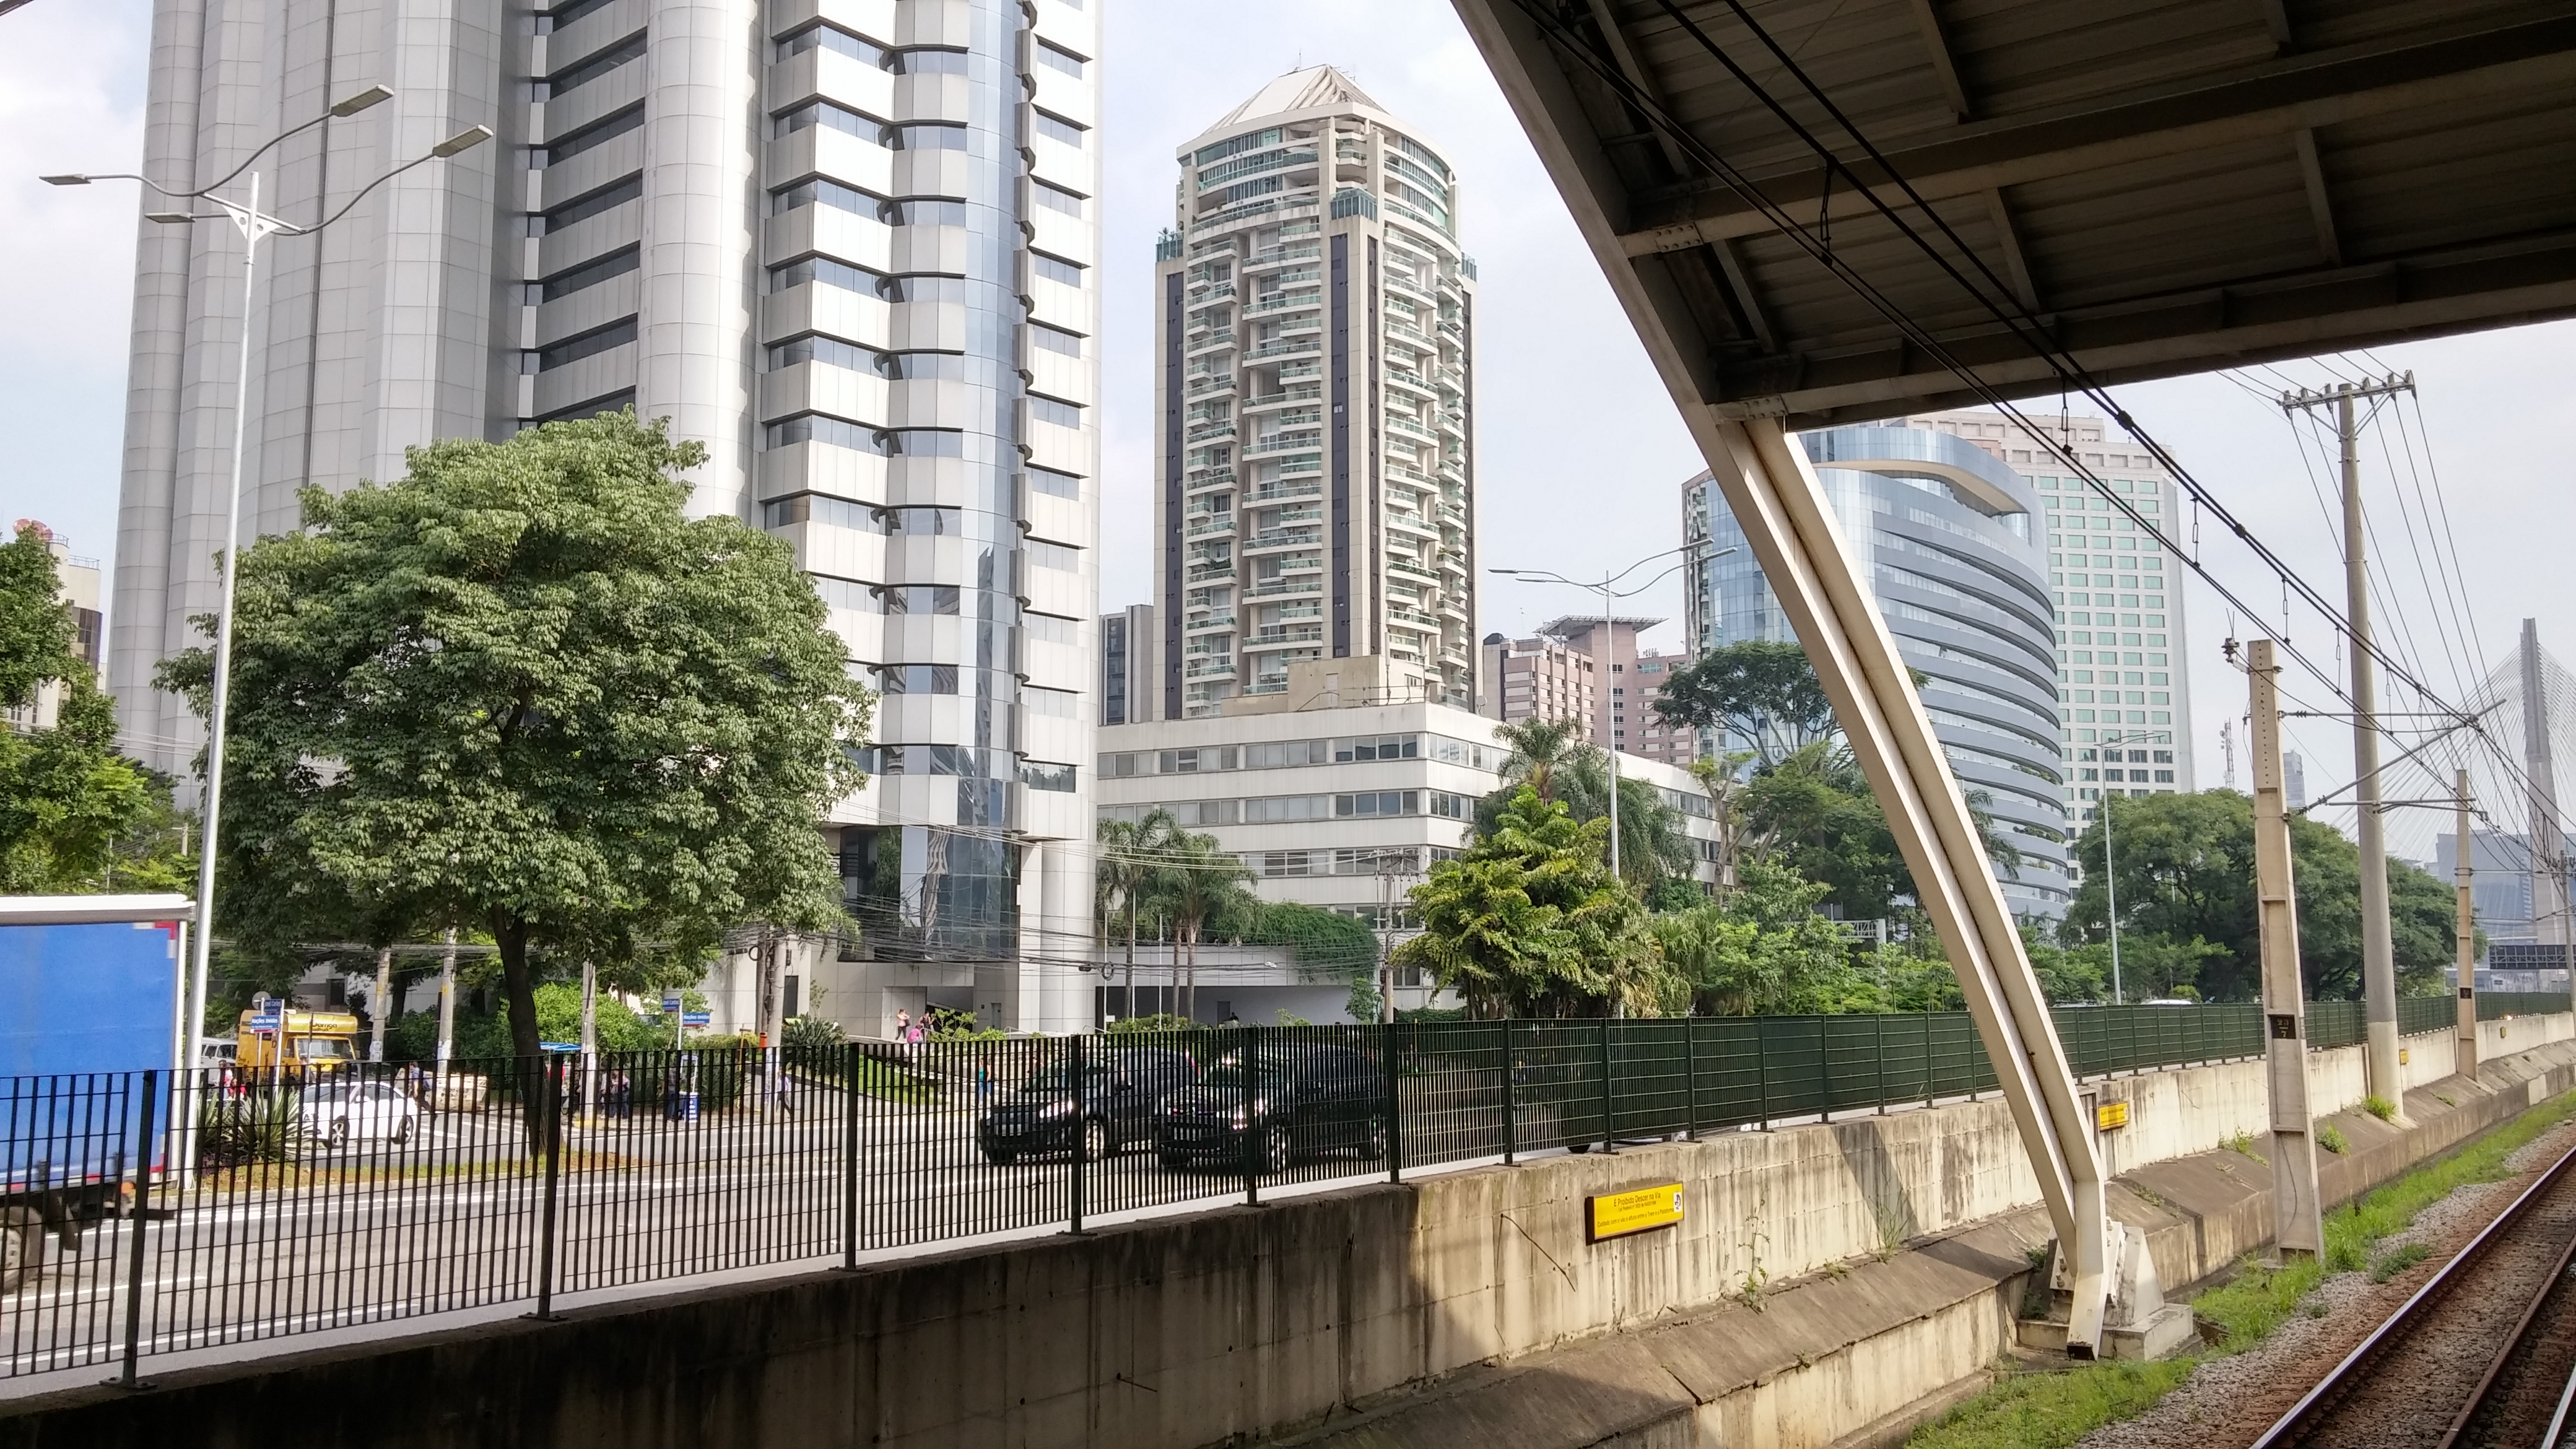
\includegraphics[keepaspectratio,width=\textwidth]{fotos/20160128_170544_HDR.jpg}
	\end{figure}
	
	O Trem Metropolitano, no caso da Linha 9-Esmeralda é interessante por dialogar tanto com a Berrini, como outras avenidas similares (em termos de ocupação do solo), como a Chucri Zaidan (Estação Morumbi) ou ainda, conjuntos de ruas e avenidas, como Funchal, Olimpíadas e Dr. Cardoso de Melo (Estação Vila Olímpia), as sete estações do miolo da Linha 9-Esmeralda,todas já mencionadas anteriormente, foram projetadas por Luiz Carlos Esteves, a respeito delas, destaco numa notícia de 22 de junho de 1998 os seguintes fragmentos:
	
	\begin{citacao}
		Até o final de setembro, a população que freqüenta alguns dos edifícios comerciais mais modernos da cidade, situados na avenida das Nações Unidas, zona sul paulistana, vai passar a contar com uma opção de transporte coletivo. Trata-se das sete novas estações de trem que a CPTM (Companhia Paulista de Trens Metropolitanos) está instalando entre as estações Pinheiros e Largo 13, pertencentes à linha C, que liga Osasco a Jurubatuba.
	
		(\dots)
	
		Luiz Esteves, arquiteto da Harza Hidrobrasileira Engenharia e Projetos, empresa responsável pela concepção e projetos de dinamização da linha Sul, aponta a segurança do usuário como um dos pontos de maior importância das novas estações. “Colocamos a área de bilheteria e catracas junto da calçada dos prédios. Dessa forma, a passarela que leva à plataforma de embarque, do outro lado da marginal, se torna uma área pagante, o que inibe a ação de delinqüentes”, explica.
	
		Outro fator que norteou o projeto, segundo Esteves, foi o urbanismo da região. “Evitamos interferir com o landscape da avenida, projetando estruturas leves e transparentes.” Componentes metálicos fechados com vidro e brises de alumínio garantiram a leveza necessária. O concreto aparece apenas em alguns momentos da estrutura, como a caixa onde serão instaladas duas escadas rolantes, uma escada fixa e um elevador para deficientes. A passarela sobre a marginal também será construída em metal, na forma de uma elipse.
		\cite{trembom}
	\end{citacao}
	
	Na altura, o investimento mencionado foi de US\$ 220 milhões, além disso, Esteves também deu detalhes das estações, então uma novidade. Por se tratar de uma notícia produzida por um periódico especializado em arquitetura, é interessante observarmos que os edifícios da região são enaltecidos ainda antes de introduzir detalhes do investimento feito pelo poder público, a partir daí, vale mencionar que, conforme \cite{Nobre}:
	
	Quanto ao investimento imobiliário, \citeonline[pág. 148]{planocentro} traça um panorama pouco superior a uma década, destacando a elevada quantidade de lançamentos imobiliários por parte do mercado:
	
	\begin{citacao}
		No período de 2002 a 2014, segundo dados da \gls{embraesp}, ocorreram 3.442 lançamentos residenciais verticais e 287 lançamentos comerciais verticais no município de São Paulo. Na Região Oeste foram 914 residenciais e 112 comerciais, sendo na Subprefeitura de Pinheiros 400 residenciais e 72 comerciais, dos quais 196 e 41, respectivamente, no distrito de Itaim Bibi. A subprefeitura de Pinheiros apresentava em 2000 uma distribuição de atividades majoritariamente residencial com 65\% de sua área construída ocupada por residências e 27\% por usos comerciais e de serviços. 
		Dados de 2014 indicam o decréscimo da predominância do uso residencial (que ainda continua predominante) para 61\% residencial e o aumento para 31\% de áreas construídas para usos comerciais e de prestação de serviços. Esta alteração de perfil se deve principalmente ao incremento de área construída comércio/serviço no distrito do Itaim Bibi onde 42\% da área construída é ocupada por estes usos. Esta transformação é explicada em parte, pelo sucesso imobiliário e pelo perfil de empreendimentos na área da \gls{ouc} Faria Lima. Neste distrito no período de 14 anos (2000 – 2014) houve o acréscimo de área construída de cerca de 2.700.000 m² de usos comércio/serviço (cerca de 64\%).
	\end{citacao}
	
	\subsection{Santo Amaro} \label{Santo Amaro}
	
	No que tange ao desenvolvimento humano e da infraestrutura, \citeonline[pág. 239]{planosul2} delinea as seguintes características:
	
	\begin{citacao}
		A deficiência na escolaridade média dos trabalhadores, o perfil etário da população bastante jovem e a pouca educação profissionalizante dos jovens geram baixos níveis salariais. A carência de emprego formal privado, com cerca de 70 mil postos de trabalho (apenas 1,6\% do total da cidade) e a pouca diversificação das atividades econômicas locais levam a grandes deslocamentos das pessoas, principalmente para outras subprefeituras, despendendo muito tempo nessas viagens. É o que ocorre no Capão Redondo, onde aproximadamente 36,1\% dos residentes gastam mais de uma hora para chegar ao local de trabalho. Isso se dá também em função do fraco desempenho do transporte público de média e alta capacidade, já que o transporte coletivo é o meio predominante para os deslocamentos nessa subprefeitura. O segundo modo de deslocamento se dá através de viagens a pé (33,6\%), que ocorre em condições de calçadas inadequadas, iluminação pública precária e segurança pública deficitária, com altos índices de homicídios por mil habitantes (22,8\%).
	\end{citacao}
	
	\begin{figure}[h]
		\caption{Plataforma da Estação Santo Amaro da Linha 9 (2013}
		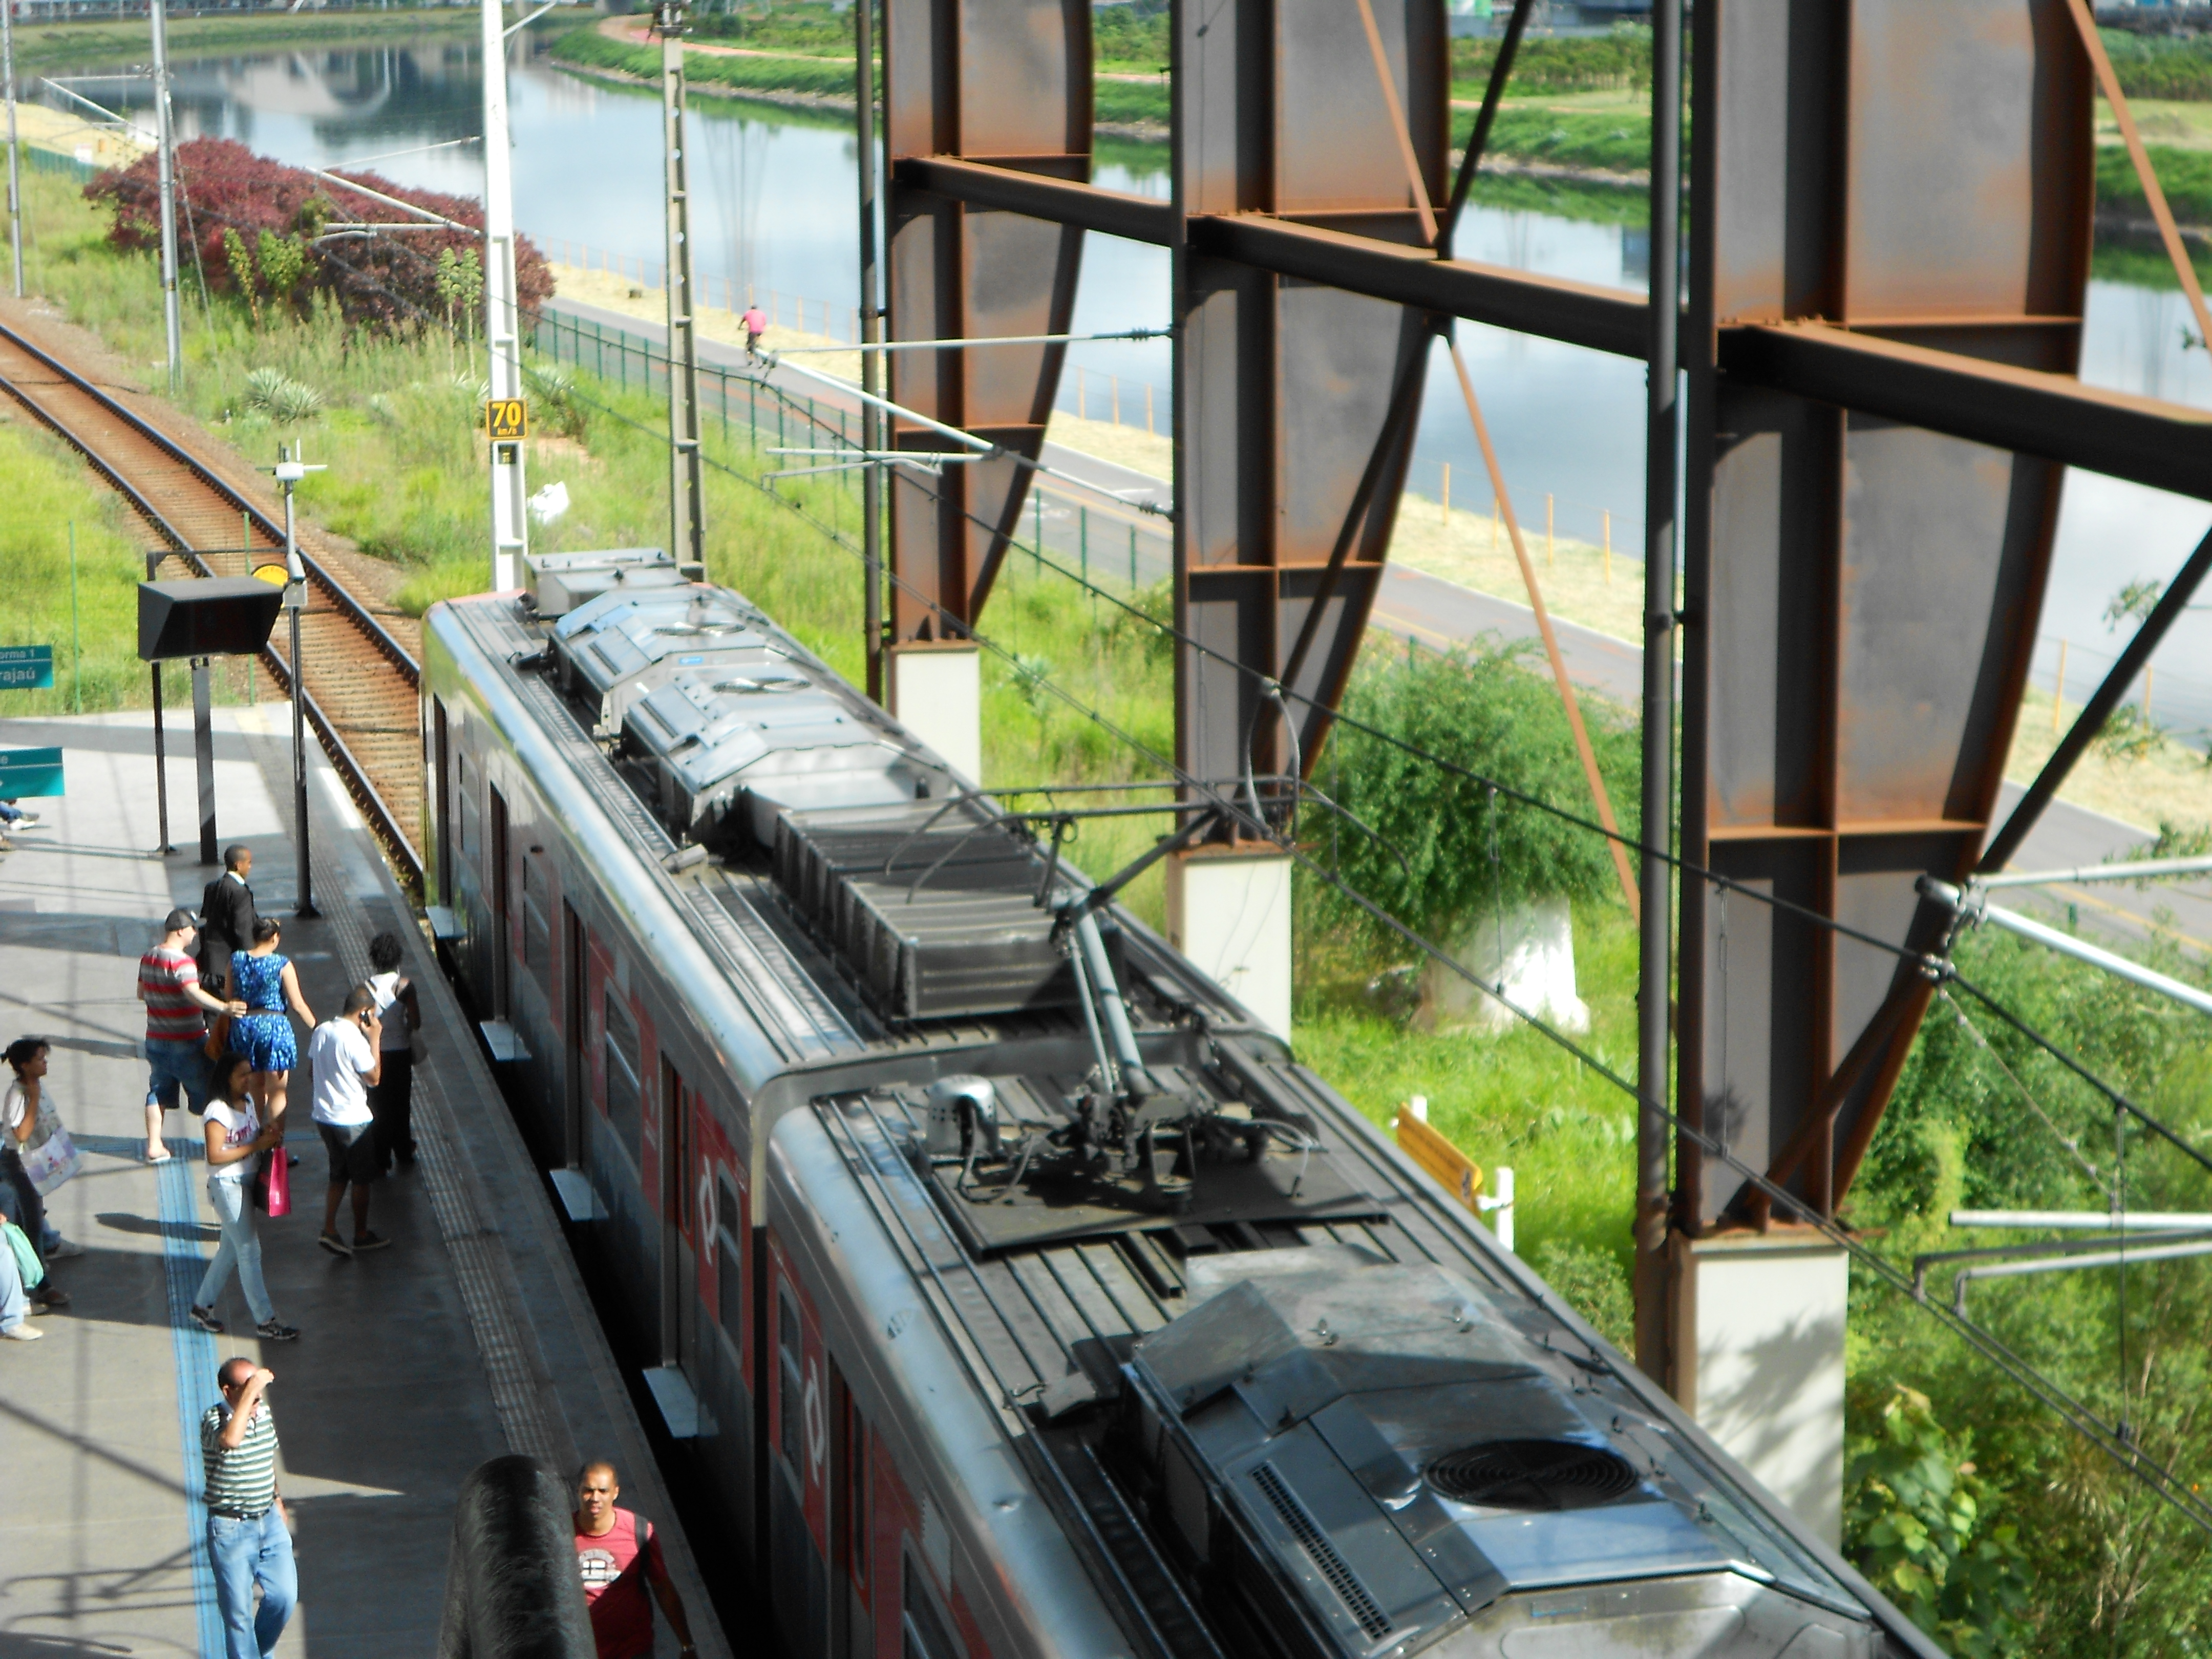
\includegraphics[keepaspectratio,width=\textwidth]{fotos/DSCN2038.jpg}
	\end{figure}	
	
	No que diz respeito ao perfil de deslocamento, \citeonline[pág. 245]{planosul2} aponta que:
	
	\begin{citacao}
		Quanto à participação das viagens geradas pelos residentes, para os três distritos municipais que conformam a Subprefeitura Santo Amaro, o destino para outras subprefeituras apresenta números relevantes (cerca de 30\%). Ainda assim, o percentual de trabalhadores que gastam mais de uma hora no deslocamento casa-trabalho (14,2\%) é inferior ao do município (21,8\%) e da macrorregião Sul 2 (26,9\%).
	\end{citacao}
	
	O baixo percentual de deslocamentos acima de uma hora podem dialogar com suas características econômicas e de infraestrutura:
	
	\begin{citacao}
		A Subprefeitura Santo Amaro integra uma região complexa, com concentração de investimentos relacionados às mais diversas manifestações econômicas - indústrias, bancos, centros financeiros, centros administrativos, hotéis, casas de espetáculos, casas de cultura, bibliotecas, redes de supermercados, escolas de todos os graus, hospitais, centro de exposições, clubes, comércio e serviços de âmbito local e regional, além de extensas áreas exclusivamente residenciais associadas a grandes manchas de vegetação.
		\cite[pág. 239]{planosul2}
		
		(\dots)
		
		Na subprefeitura Santo Amaro o uso e ocupação do solo é bastante diversificado, com predominância de áreas de uso misto, extensas áreas de uso estritamente residencial, áreas de centralidade e áreas de uso industrial em transformação ao longo dos eixos da Marginal do Rio Pinheiros e do Canal Jurubatuba. É nesse setor que se verifica a potencialidade de instalação de comércio e serviços de grande porte, com acesso regional e metropolitano, seja pela presença de terrenos com dimensões propícias a grandes empreendimentos, seja pela acessibilidade facilitada com a existência de eixos viários, transposições e sistema de transporte ferroviário. Apresenta, também, áreas ocupadas por clubes esportivos sociais e de campo, integrantes do Sistema de Áreas Protegidas, Áreas Verdes e Espaços Livres (\gls{sapavel}).
		\cite[pág. 243]{planosul2}
	\end{citacao}
	
	\begin{figure}[h]
		\caption{Estação Socorro observada a partir do mezanino da Estação Santo Amaro (2013}
		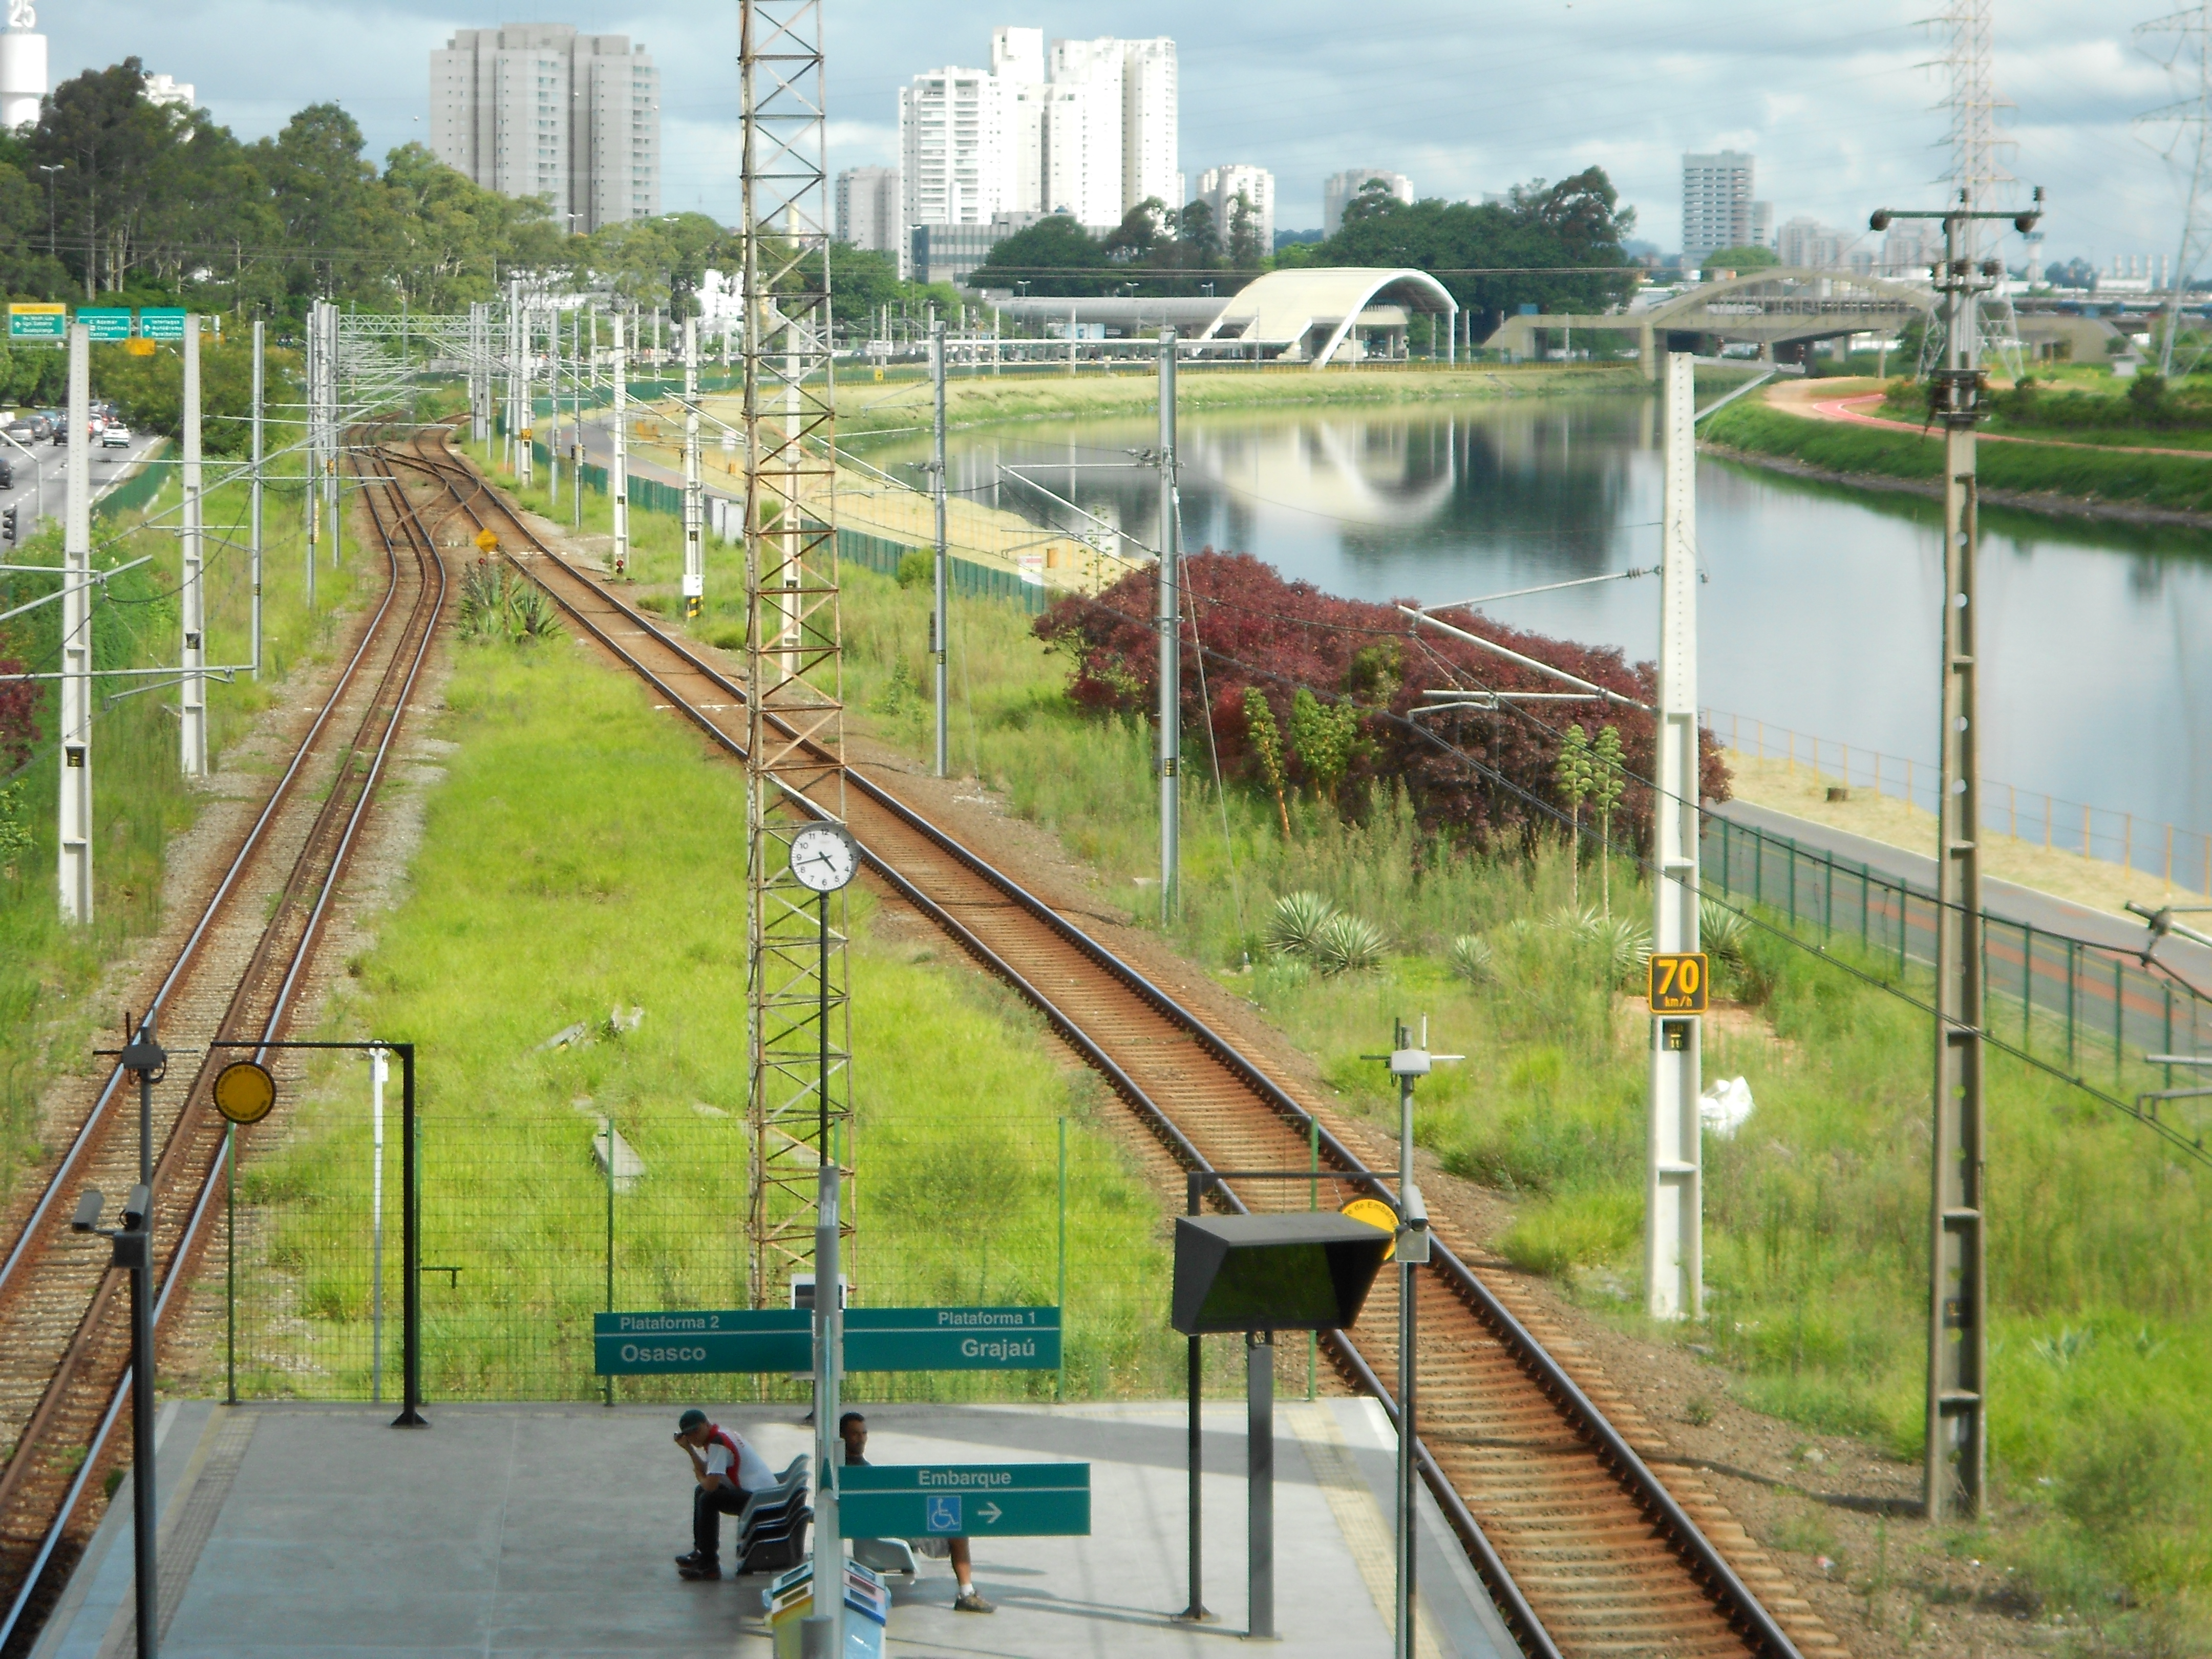
\includegraphics[keepaspectratio,width=\textwidth]{fotos/DSCN2027.jpg}
	\end{figure}
	
	\subsection{Capela do Socorro}
	
	Conforme \citeonline[pág. 101]{planosul2}, a localização e infraestrutura de circulação da Prefeitura Regional são caracterizadas da seguinte maneira:	``a Subprefeitura de Capela do Socorro, localizada na macrorregião Sul 2, desenvolve-se a partir do centro regional de Santo Amaro, estando associada ao vetor de urbanização sudoeste da cidade de São Paulo e estruturada pelos eixos viários da Avenida Washington Luiz, dando seqüência a Avenida Victor Manzini, Avenida Interlagos, Avenida Atlântica e Avenida Rio Bonito''.
	
	\citeonline[pág. 101]{planosul2} também descreve a ocupação do solo da região e comenta sobre o uso do solo, como podemos observar a seguir:
	
	\begin{citacao}
		A ocupação do território da subprefeitura organiza-se através dos vetores de urbanização ao longo das vias e, de nucleações dispersas que se articulam através de um sistema viário secundário marcado pelo uso residencial. Essas nucleações ao sul estão entremeados por fragmentos descontínuos da mata atlântica além de chácaras e sítios de produções hortifrutigranjeiras. Parte do distrito de Socorro, situada ao norte dos reservatórios Billings e Guarapiranga, apresenta uma ocupação urbana consolidada, composta por extensos bairros residenciais de padrões urbanos de classe média, entremeados por centralidades lineares como Avenida Atlântica, ou centralidades polares como o Largo do Socorro. O uso industrial é uma atividade importante nas proximidades do Largo do Socorro, aparecendo também de forma mais difusa no distrito de Socorro e Cidade Dutra.
	\end{citacao}
	
	\citeonline[pág. 103]{planosul2} também destaca características quanto ao perfil do solo em área de proteção de manancial, sendo importante mencionar que a estação apontada com o nome ``Novo Varginha'' pelo plano regional não se encontra edificada até o presente momento:
	
	\begin{citacao}
		A orla do Reservatório Guarapiranga está associada à atividades de lazer e recreação, destacando-se a recente implementação de parques urbanos,também áreas de interesse cultural tombadas pelo \gls{condephaat}, os bens arquitetônicos Yacht Club Santa Paula e seu anexo à garagem de barcos. Em direção ao Sul nota-se um adensamento da urbanização seccionada pela Linha Esmeralda da CPTM, à leste da ferrovia observa-se um forte adensamento populacional e construtivo marcado pela precariedade ambiental e urbana. Sobre as infraestruturas de transporte planejadas pelo \gls{pde} (Plano Diretor Estratégico),destacam-se o corredor de ônibus da Avenida Belmira Marin e a extensão da Linha Esmeralda da \gls{cptm} até a Estação Novo Varginha.
	\end{citacao}
	
	Quanto à caracterização do perfil de viagens\footnote{Observa-se aqui um tom que valoriza a Linha 5 em detrimento da Linha 9, reforçando uma visão sobre o transporte sobre trilhos que o presente trabalho contraria, visto que a conexão com a Linha 5, de abrangência limitada até os dias atuais, não deve ser supervalorizada apenas por posições de cunho pessoal, ligadas ao posicionamento institucional das estatais responsáveis pelas malhas que compõem o sistema metroferroviário. Vale observar que as viagens atraídas exigem o uso da Linha 9, não da Linha 5}:
	
	\begin{citacao}
		O modal mais utilizado nas viagens desta subprefeitura é o transporte motorizado coletivo e individual, respectivamente, onde cerca de 36\% da população gasta mais de 1 hora nas viagens diárias, os habitantes de Capela do Socorro são servidos pela Linha Esmeralda da CPTM, até a Estação Grajaú. No entanto, somente através de Campo de Limpo ou Santo Amaro podem ter acesso a Linha Lilás do Metrô. Segundo a pesquisa de origem e destino OD, o território de Capela do Socorro atrai viagens da própria subprefeitura e de outras como Santo Amaro, Pinheiros e a subprefeitura da Sé. \cite[pág. 106]{planosul2}
	\end{citacao}
	
	\section{Linha 5-Lilás}
	
	\subsection{Campo Limpo}
	
	Conforme \citeonline[pág. 61]{planosul2}, a Prefeitura Regional pode ser caracterizada da seguinte maneira:
	
	\begin{citacao}
		A Subprefeitura de Campo Limpo integra a Macrorregião Sul 2 do Município de São Paulo e é composta pelos Distritos Vila Andrade, Campo Limpo e Capão Redondo. Ocupa uma área total de 36,7 km² e abriga população de 607.105 habitantes. Faz divisa com as seguintes subprefeituras: ao norte com Butantã, ao sul com M’Boi Mirim, a leste com esta última e Santo Amaro. A divisa a oeste se dá com os municípios de Taboão da Serra, Embu e Itapecerica da Serra.
		
		(\dots)
		
		A partir da década de 1990, como em Vila Andrade, ocorreu grande crescimento imobiliário com o lançamento de empreendimentos residenciais para a classe média. Em face de sua proximidade a centros comerciais, escritórios, ao distrito de Vila Andrade e bairros como o Morumbi, Campo Limpo começou a atrair novos moradores com nível superior, profissionais liberais e originários de outras regiões da cidade, interessados em imóveis mais baratos e próximos às novas áreas de trabalho. A partir de 2001, iniciou-se novo crescimento com a instalação de empreendimentos comerciais e educacionais.
	\end{citacao}
	
	O transporte coletivo está presente como elemento estruturador:
	
	\begin{citacao}
		Em relação aos elementos estruturadores, além do Arco Faria Lima – Águas Espraiadas – Chucri Zaidan e do Arco Jurubatuba, situados na MEM, o PDE apresenta a rede estrutural de transporte coletivo, formada pelo eixo de transformação urbana da área de influência do Corredor de ônibus Itapecerica/ João Dias/ Centro e do previsto Capão Redondo/ Campo Limpo/ Vila Sônia (já em implantação na Subprefeitura de Butantã) no eixo formado pela Estrada do Campo Limpo e Avenida Carlos Lacerda (o projeto prevê conexão entre o Terminal Campo Limpo e o Terminal Capelinha, sendo este localizado nas proximidades da Estação Capão Redondo do Metrô) e pela Linha 5 Lilás do Metrô, por meio das estações Giovanni Gronchi, Vila das Belezas, Campo Limpo e Capão Redondo. A rede hídrica e ambiental é formada pelos parques urbanos e lineares já citados.
		\cite[pág. 63]{planosul2}
	\end{citacao}
	
	O plano regional publicado em 2016 dá conta de que os ``três distritos dessa Subprefeitura baseiam sua economia na prestação de serviços e no comércio. O distrito de Capão Redondo possui um índice de emprego no setor industrial (10,5\%) um pouco mais expressivo que os demais distritos'' \cite[pág. 64]{planosul2}. Um maior detalhamento do perfil da oferta de empregos pode ser visto a seguir:
	
	\begin{citacao}
		Os empregos da subprefeitura se concentram no setor de serviços, (49,1\%), seguido pelos setores comercial (29,3\%), construção civil (9,1\%), industrial (7,8\%). Vila Andrade possui 57,2\% dos empregos no setor de prestação de serviços, 28,1\% no setor comercial, 6,9\% no setor de construção civil e 5,5\% no setor industrial. No Campo Limpo, 44,7\% dos empregos estão no setor de prestação de serviços, 32,6\% no comércio, 14,5\% na construção civil e apenas 7,9\% na indústria. No Capão Redondo, 42,7\% dos empregos encontram-se no setor de serviços, 28,0\% no comércio, 10,5\% no setor industrial e 7,4\% no setor de construção civil. \cite[pág. 64]{planosul2}
	\end{citacao}
	
	Quanto à caracterização do perfil de uso do transporte coletivo:
	\begin{citacao}
		Em 2007, como resultado da pesquisa Origem e Destino do Metrô, o modo de transporte mais utilizado na subprefeitura é o coletivo (44,4\%) seguido pelo “a pé” (31,7\%), pelo individual (23,3\%) e pela bicicleta (0,6\%). O Capão Redondo é onde o transporte coletivo é mais usado (51,6\%), seguido pelo “a pé“ (32,5\%) e pelo individual (15,9\%) e a bicicleta é considerada como não utilizada. No Campo Limpo essa tendência permanecia igual ao Capão Redondo. No entanto, na Vila Andrade o modo predominante é o individual (39,9\%), seguido pelo coletivo (31,9\%), “a pé” (27,7\%) e por último a bicicleta (0,6\%). Em 2010, dos moradores desta subprefeitura, 29,2\% gastavam mais de uma hora no deslocamento casa – trabalho. Esse percentual é bem acima do que é encontrado em média no município (21,8\%) e até mesmo na região Sul 2 (25,7\%). O distrito onde esse percentual é maior é Capão Redondo e o menor é Vila Andrade. No Campo Limpo, é de 27,1\%.” \cite[pág. 66]{planosul2}
	\end{citacao}
	
	Quanto à caracterização do perfil de viagens:
	\begin{citacao}
		Das viagens geradas no Campo Limpo, 41\% são para o próprio distrito, 33\% para outras subprefeituras), com destaque para Pinheiros (11\%), Santo Amaro (9\%) e M’Boi Mirim (6\%). Entre as viagens geradas no distrito de Capão Redondo, as principais são para outros distritos (36\%), seguidas de 33\% para o próprio distrito, Santo Amaro (14\%) Pinheiros (9\%), e M’Boi Mirim (8\%). As viagens geradas em Vila Andrade têm como principal destino  outros distritos (33\%), o próprio distrito (22\%), Butantã (20\%), Pinheiros (15\%), Santo Amaro (10\%). \cite[pág. 67]{planosul2}
	\end{citacao}
	
	Quanto ao desenvolvimento humano:
	
	\begin{citacao}
		A deficiência na escolaridade média dos trabalhadores, o perfil etário da população bastante jovem e a pouca educação profissionalizante dos jovens geram baixos níveis salariais. A carência de emprego formal privado, com cerca de 70 mil postos de trabalho (apenas 1,6\% do total da cidade) e a pouca diversificação das atividades econômicas locais levam a grandes deslocamentos das pessoas, principalmente para outras subprefeituras, despendendo muito tempo nessas viagens. É o que ocorre no Capão Redondo, onde aproximadamente 36,1\% dos residentes gastam mais de uma hora para chegar ao local de trabalho. Isso se dá também em função do fraco desempenho do transporte público de média e alta capacidade, já que o transporte coletivo é o meio predominante para os deslocamentos nessa subprefeitura. O segundo modo de deslocamento se dá através de viagens a pé (33,6\%), que ocorre em condições de calçadas inadequadas, iluminação pública precária e segurança pública deficitária, com altos índices de homicídios por mil habitantes (22,8\%). \cite[pág. 68]{planosul2}
	\end{citacao}
	
	\subsection{Santo Amaro}
	
	Devido à baixa penetração da Linha 5 na Prefeitura Regional, com as estações Santo Amaro (integração com a Linha 9-Esmeralda, já abordada no capítulo \ref{L9}), Largo Treze e Adolfo Pinheiro, indicamos a leitura da seção \ref{Santo Amaro} para maiores detalhes.

	\noindent
	\begin{minipage}[b]{.4\textwidth}
		\captionof{figure}{Canteiro de obras da Estação Adolfo Pinheiro, 2013}
		\includegraphics[width=\linewidth]{fotos/DSCN0424.jpg}
	\end{minipage}%
	\hfill
	\begin{minipage}[b]{.4\linewidth}
		\captionof{figure}{Túneis da Linha 5 na região da Estação Adolfo Pinheiro durante as obras, 2013}
		\includegraphics[width=\textwidth]{fotos/DSCN0488.jpg}
	\end{minipage}	
	
	\subsection{M’Boi Mirim}
	
	Conforme \citeonline[pág. 146]{planosul2}, a Prefeitura Regional pode ser caracterizada da seguinte maneira:
	
	\begin{citacao}
		A Subprefeitura M’Boi Mirim integra a Macrorregião Sul 2 do Município de São Paulo e é composta pelos distritos Jardim Ângela e Jardim São Luís. Ocupa área total de 62,10 km² e abriga população de 563.305 habitantes.1 Faz divisa com as seguintes subprefeituras: ao norte com Campo Limpo, ao sul com Parelheiros e a leste com Santo Amaro e Capela do Socorro. A oeste a fronteira se faz com o município de Itapecerica da Serra.
	\end{citacao}
	
	Quanto ao processo de ocupação da região:
	
	\begin{citacao}
		Neste meio físico se expandiram desordenadamente núcleos urbanos adensados, com padrões de implantação e sanitários bastante precários, com drenagem deficiente e ausência de esgotamento sanitário, em áreas com risco de erosão e de inundação. O território do Jardim Ângela foi ocupado de forma desordenada, com construções irregulares e precárias. O Jardim São Luís, por outro lado, embora com ocupações desordenadas, construções precárias e algumas áreas de risco, apresenta também áreas com padrão de ocupação mais ordenado e predominantemente horizontal. \cite[pág. 147]{planosul2}
	\end{citacao}
	
	Quanto à caracterização do perfil de deslocamento da população:
	
	\begin{citacao}
		Também em 2007, 34,2\% dos moradores desta subprefeitura gastavam mais de uma hora no deslocamento casa-trabalho. Esse percentual encontra-se bem acima da média do município (21,8\%) e até mesmo região Sul 2 (25,7\%). 43\% das viagens geradas no Jardim Ângela eram para o próprio distrito, seguido por Santo Amaro (14\%), Pinheiros (7\%), Vila Mariana (7\%) e outras subprefeituras (29\%). No Jardim São Luís, 39\% das viagens eram para o próprio distrito, seguido para Santo Amaro (16\%), Pinheiros (9\%), Vila Mariana (8\%) e para outras subprefeituras (28\%). No Jardim Ângela, a proporção de viário estrutural sobre o viário total é 4,7\% e no Jardim São Luís de 11\%. A proporção de corredores de ônibus sobre o viário total nessa subprefeitura é de 1,5\%, semelhante à região Sul 2 (1,2\%) e acima ao existente no município (0,7\%). O Jardim Ângela não possui ciclovias, porém no distrito de Jardim São Luís a proporção é de 1,1\%. \cite[pág. 147]{planosul2}
	\end{citacao}
	
	O atendimento desta Prefeitura Regional por parte do sistema de trilhos se limita à Estação Giovanni Gronchi.
	
%
%==============================================================================================	
%

	\chapter{Metodologia e resultados}
	
	\section{Da teoria}
	
	Com relação à adoção da infraestrutura de transporte sobre trilhos como indutora de transformações urbanas, nos baseamos na posição de \citeonline{Barbosa} com base em fontes secundárias:
	
	\begin{citacao}
		A questão da acessibilidade e consequentemente dos transportes também
		aparece como uma hipótese importante. Segundo essa hipótese, áreas com
		boa acessibilidade teriam maior tendência tanto a serem ocupadas
		rapidamente como a sofrerem transformações mais intensas, atraindo,
		sobretudo, a verticalização e o comércio/serviços.
		
		Obviamente essa “boa acessibilidade” é relativa aos interesses dos diversos
		setores da sociedade. Assim, por exemplo, áreas bem servidas pelas ferrovias
		e posteriormente rodovias foram interessantes para o uso industrial e para o
		uso residencial operário
		\apud[pág. 26 / pág. 233, pág. 356]{Barbosa}{Mendes}
		\apud[pág. 26 / pág. 158]{Barbosa}{Taralli}
		\apud[pág. 26 / pág. 32]{Barbosa}{Segatto}
		\apud[pág. 26 / pág. 1026]{Barbosa}{Ernani}
	\end{citacao}

	\section{Da definição da área de estudo}
	
	Considerando a revisão teórica e as dimensões próprias e características heterogêneas da capital paulista e da Região Metropolitana de São Paulo, fez-se necessário limitar a área de estudo, para tanto selecionamos as Prefeituras Regionais ligadas ao vetor sudoeste e a infraestrutura de transporte sobre trilhos associada, o que significou as linhas: 5-Lilás da \gls{cmsp}, 8-Diamante e 9-Esmeralda da \gls{cptm}. Foram fatores determinantes:
	\begin{itemize}
		\item O crescimento e desenvolvimento imobiliário nas últimas décadas, sobretudo dentro do período para o qual foram aplicadas técnicas de sensoriamento remoto com base em imagens dos satélites Landsat 4 e 5, que operaram eficientemente entre 1982 e 2011;
		\item A presença de infraestrutura de transporte sobre trilhos de alta capacidade, que apresentou evolução no que diz respeito à oferta de lugares;
		\item A presença de múltiplos centros (alguns deles subcentros), sendo possível afirmar que subcentros como a Lapa surgiram a partir da chegada da ferrovia, possível de ser evidenciado a partir da comparação cartográfica entre o segmento das pesquisas Origem Destino dos anos de 1997 e 2007 que diz respeito às viagens atraídas por motivo, principalmente trabalho.
	\end{itemize}
	
	\section{Das técnicas de cartografia e geoprocessamento}
	
	Na representação das viagens atraídas por motivo de trabalho nas áreas de indústria, comércio e serviços divididas por subprefeituras regionais, foi utilizado o QGIS. Para tanto, foram utilizados os dados da Pesquisa Origem Destino dos anos de 1997 e de 2007, afim de comparar a influência das linhas \gls{cptm} e \gls{cmsp} na expansão da malha urbana da região estudada e do GeoSampa, que disponibiliza o shapefile das prefeituras regionais do município. Após recortar a área de estudo, integramos os dados das zonas da origem-destino aos da tabela de viagens atraídas por motivo (sendo selecionados dos motivos de trabalho). Assim, integramos a tabela produzida ao \textit{shapefile} das prefeituras regionais. A partir disso, dissolvemos os polígonos das zonas da Pesquisa Origem Destino somando seus dados, com o objetivo de representá-los divididos por subprefeituras. Foram empregados, assim, os recursos: recorte, união, mesclagem, intersecção e edição de tabelas.
	
	Dissolver os dados das zonas nos polígonos das prefeituras regionais, somando-os.
	
	\section{Das técnicas de sensoriamento remoto}
	
	O avanço da área urbana no entorno da malha ferroviária é evidenciado à partir da comparação entre imagens obtidas por sensoriamento remoto antes, durante e depois da construção e integração das linhas 8 e 9 da \gls{cptm} à linha 5, da \gls{cptm}. Optamos por imagens dos satélites Landsat 4 e 5 devido o período de operação, que abrange o intervalo de tempo analisado \textemdash entre 1982 e 2011.
	
	Utilizando o programa Envi, fizemos a escolha por três composições de bandas para analisar a área de estudo nos anos de 1985, 1990, 2000 e 2010:
	
	\begin{itemize}
		\item 3-2-1: fornece uma visualização muito aproximada do aspecto natural da área, onde a vegetação aparece em tons de verde e características urbanas são reveladas pelas cores branca, cinza, azul e roxa;
		\item 4-3-2: nessa composição, a vegetação aparece em tons de vermelho e mancha urbana em tons de branco e ciano claro, demonstrando assim o avanço da mancha urbana; nota-se que a urbanização ocorre de forma mais intensa à margem leste do Rio Pinheiros;
		\item 5-4-3: funciona, como ocorre na composição 4-3-2, por contraste de cores. nesse caso, a fim de evidenciar a vegetação, que aparece em tons de verde claro. Permite, portanto, demonstrar a redução da vegetação à medida da densificação urbana.
	\end{itemize}

%
%==============================================================================================
%

	\chapter{Conclusão}
	
	O presente trabalho permitiu ``costurar'' melhor alguns conceitos apresentados pela disciplina, de forma a garantir sua fixação. Foi possível estabelecer relações para além da bibliografia básica, mas sempre mantendo a transversalidade. Confirmamos os apontamentos indicados pela revisão teórica e pesquisa empírica, evidenciando também a forte heterogeneidade presente no território.
	
%	Fica também evidente a heterogeneidade não só da capital ou da \gls{rmsp}, mas da própria malha do Trem Metropolitano, o que se deve, como vimos, a heranças de estatais diferentes, cada qual com seu contexto histórico particular.
	
	% ----------------------------------------------------------
	% ----------------------------------------------------------
	\postextual
	
	
	
	% informa o arquivo com a bibliografia. Deve ser o mesmo nome
	% (sem o sufixo) que será informado no ambiente filecontents
	% que está no final deste arquivo. Neste exemplo foi usado 
	% bibitemp.bib e bibtemp. Este comando insere a bibliografia
	% nesta posição (antes dos apêndices, anexos, índice remissivo)
	\bibliography{referencias}
	% ----------------------------------------------------------
	% Glossário
	% ----------------------------------------------------------
	% Consultar manual da classe abntex2 para orientações sobre o
	% uso do glossário.
	\renewcommand{\glossaryname}{Glossário}
	%\renewcommand{\glossarypreamble}{Esta é a descrição do glossário.\\ \\}
	\renewcommand*{\glsseeformat}[3][\seename]{\textit{#1}
	\glsseelist{#2}}

	% ---
	% Traduções para o ambiente glossaries
	% ---
	\providetranslation{Glossary}{Glossário}
	\providetranslation{Acronyms}{Siglas}
	\providetranslation{Notation (glossaries)}{Notação}
	\providetranslation{Description (glossaries)}{Descrição}
	\providetranslation{Symbol (glossaries)}{Símbolo}
	\providetranslation{Page List (glossaries)}{Lista de Páginas}
	\providetranslation{Symbols (glossaries)}{Símbolos}
	\providetranslation{Numbers (glossaries)}{Números} 
	% ---
	
	% ---
	% Imprime o glossário
	% ---
	\cleardoublepage
	\phantomsection
	\addcontentsline{toc}{chapter}{\glossaryname}
	% \glossarystyle{index}
	% \glossarystyle{altlisthypergroup}
	\glossarystyle{tree}
	\printglossaries
	% ---
	
	% ----------------------------------------------------------
	% Apêndices
	% ----------------------------------------------------------
	
	% ---
	% Inicia os apêndices. Não esquecer de fechar ao final de
	% todos os apêndices (\end{apendicesenv})
	% ---
	%\begin{apendicesenv}
	
	% Imprime uma página indicando o início dos apêndices
	%\partapendices
	
	% ----------------------------------------------------------
	%\chapter{Primeiro apêndice}
	% ----------------------------------------------------------
	
	%Este é um exemplo de inclusão de capítulos de %apêndice em uma 
	%monografia.  Cada apêndice é tratado como se fosse %um capítulo.
	%Os apêndices devem ser iniciados pelo comando de %ambiente
	%\textbackslash begin\{apendicesenv\} e encerrados %pelo comando 
	%\textbackslash end\{apendicesenv\}.
	
	% ----------------------------------------------------------
	%\chapter{Segundo apêndice}
	% ----------------------------------------------------------
	
	%Este é um exemplo de inclusão de um segundo apêndice. 
	
	%\end{apendicesenv}
	% ---
	
	
	% ----------------------------------------------------------
	% Anexos
	% ----------------------------------------------------------
	
	% ---
	% Inicia os anexos
	% ---
	%\begin{anexosenv}
	
	% Imprime uma página indicando o início dos anexos
	%\partanexos
	
	% ---
	%\chapter{Primeiro anexo}
	% ---
	%Os anexos são similares aos apêndices se distinguindo pelo fato
	%que os apêndices são de autoria do autor da monografia e os 
	%anexos não são da autoria do autor da monografia.  Por exemplo,
	%se incluir no trabalho um modelo de um formulário preenchido
	%por alunos participantes de uma pesquisa, este será um apêndice
	%se o formulário foi criado pelo autor da monografia e será um
	%anexo se o formulário tiver sido criado por outros (por exemplo,
	%é um formulário padrão da escola em que o aluno que o preenche
	%estuda).
	%
	%Mesmo que o formulário tenha sido elaborado pela escola, uma
	%reprodução do formulário preenchido por cada aluno na pesquisa
	%será incluído no apêndice pois envolve o trabalho do autor da
	%monografia ao distribuir, coletar e reproduzir as respostas.
	%
	%Este é um exemplo de inclusão de capítulos de anexos em uma 
	%monografia.  Cada anexo é tratado como se fosse um capítulo.
	%Os anexos devem ser iniciados pelo comando de ambiente
	%\textbackslash begin\{anexoenv\} e encerrados pelo comando 
	%\textbackslash end\{anexoenv\}.
	%
	%\end{anexosenv}
	% ---
	%---------------------------------------------------------------------
	%---------------------------------------------------------------------
	
	%\printindex
	
	% Por padrão são incluídas no trabalho somente as referências
	% citadas ao longo do texto. No comando abaixo foram acrescentadas
	% algumas referências não citadas (neste texto servem apenas como
	% exemplos). Não deve ser usado o comando (mais simples) 
	% \nocite{*}, pois este parece não ser compatível com o
	% abntex2cite
	%\nocite{abntex2cite,abntex2wiki,boyer,eves,iezzi,kletenic,
	%        diomara,steinbruch,intusolatex,feynman,shannon,
	%        luisfelipe,turing}
\end{document}
